\documentclass[a4paper,12pt]{book}%{report}
%
\usepackage{a4wide}
\usepackage[amssymb]{SIunits}
\usepackage{units}
\usepackage{pslatex}
\usepackage{amssymb}
\usepackage{amsbsy}
\usepackage[fleqn]{amsmath}
\usepackage{bbm}
\usepackage{mathtools}
\usepackage{booktabs}
\usepackage{url}
\usepackage[many]{tcolorbox} %Achtung! Reihenfolge beachten
\usepackage{xcolor}
\usepackage[utf8]{inputenc}
\usepackage[ngerman]{babel} % needs: sudo apt-get install texlive-lang-german
\usepackage[figurename=Abb.]{caption}
\usepackage{calrsfs}
\usepackage[titletoc]{appendix}
\usepackage{thumbpdf}
\usepackage[colorlinks,
pdfpagelabels,
pdfstartview = FitH,
bookmarksopen = true,
bookmarksnumbered = true,
linkcolor = black,
plainpages = false,
hypertexnames = false,
citecolor = black]{hyperref}
% Define the headers
\usepackage{fancyhdr}
\pagestyle{fancy}
\fancyhf{}
\fancyhead[EL]{\leftmark}
\fancyhead[OR]{\rightmark}
\fancyfoot[OR]{\thepage}
\fancyfoot[EL]{\thepage}
\renewcommand{\headrulewidth}{0pt}
% This is to have text flow around figures
\usepackage{wrapfig}
% Use tikz and pgfplot thru gnuplot
\usepackage[miktex]{gnuplottex}
\usepackage{gnuplot-lua-tikz}
\usepackage{tikz}
\usepackage{circuitikz}
\usepackage{pgfplots}
%\pgfplotsset{compat=1.14}
\usetikzlibrary{decorations.pathmorphing,decorations.pathreplacing,decorations.markings,patterns} %,snakes}
\usetikzlibrary{shapes,arrows,chains,matrix,positioning,scopes}
\usetikzlibrary{positioning}
\usetikzlibrary{calc}
\usetikzlibrary{arrows.meta}
\tikzset{darkstyle/.style={circle,draw,fill=gray!40}}
%colours
\definecolor{darkgreen}{rgb}{0,0.6,0}
\newcommand{\dgreen}{\color{darkgreen}}
\newcommand{\red}{\color{red}}
\newcommand{\blue}{\color{blue}}
\newcommand{\cyan}{\color{cyan}}
\newcommand{\green}{\color{green}}
\newcommand{\mbs}[1]{\ensuremath{\boldsymbol{\mathbf{#1}}}}
% New command and renewcommand settings
\newcommand{\mbf}{\mathbf}
\newcommand{\bs}{\boldsymbol}
%\renewcommand{\thepage}{{\thepart}.\arabic{page}}
%\addto\captionsgerman{\renewcommand{\figurename}{Abb.}}
\newtheorem{theorem}{Satz}
% New environment settings
%
\definecolor{myblue}{RGB}{0,163,243}
\tcbset{mystyle/.style={ 
%  breakable, 
  enhanced, 
  outer arc=0pt, 
  arc=0pt, 
  colframe=gray, 
  colback=white, 
  boxed title style={ 
    colback=gray,
    coltitle=black,
    colbacktitle=gray,
  }, 
  outer arc=5pt,
  title=Boxhead~\thetcbcounter, 
  fonttitle=\sffamily 
  } 
}
%
\newtcolorbox[auto counter]{satz}[1]{mystyle, title=Satz~\thetcbcounter: #1}
\newtcolorbox[auto counter]{exercise}[1]{mystyle, title=Aufgabe~\thetcbcounter: #1}
\newtcolorbox[auto counter]{example}[1]{breakable,mystyle, title=Beispiel~\thetcbcounter: #1}
\newtcolorbox{note}[1]{ enhanced,attach boxed title to top left={yshift=-3mm,yshifttext=-1mm},
  title={N.B.: #1},fonttitle=\bfseries,
  boxed title style={size=small}}
%
\newboolean{showComments} %Textblöcke anzeigen
\newcommand\Comment[1]{\ifthenelse{\boolean{showComments}}{\leavevmode\newline{\blue #1}\newline}{}}
%
\newboolean{showErratum} %Textblöcke anzeigen
\newcommand\Erratum[1]{\ifthenelse{\boolean{showErratum}}{\leavevmode\newline{\red #1}\newline}{}} 
%
%\title{\huge Lecture Notes\\
%\large für Studierende der Studiengänge Embedded Systems %Engineering, Mirkosystemtechnik und Sustainable Systems %Engineering}
%\author{Andreas Greiner und Lars Pastewka \\Professur für %Simulation\\Institut für Mikrosystemtechnik\\Universität %Freiburg}
\parindent0em
\parskip1ex
\pagestyle{headings}
\setcounter{secnumdepth}{3}
% The following is better placed in the main document
%\setboolean{showComments}{true}
%\setboolean{showErratum}{true}
\parindent0em
\parskip1ex
\pagestyle{headings}
% We want the mathindent to be zero.
%\setlength{\mathindent}{0cm}
\setboolean{showComments}{false}
\setboolean{showErratum}{false}
%
\title{\huge Lecture Notes\\
\large für Studierende der Studiengänge Embedded Systems Engineering, Mirkosystemtechnik und Sustainable Systems Engineering}
\author{Andreas Greiner und Lars Pastewka \\Professur für Simulation\\Institut für Mikrosystemtechnik\\Universität Freiburg\\[1cm]
  
\includegraphics[width=0.4\textwidth]{fig/Uni_Logo-Grundversion_E1_A4_RGB}
}
%
%\usepackage{caption}
%\usepackage{lipsum}
%\usepackage{cutwin}
%
\begin{document}
\frontmatter
\maketitle
\part{Differentialgleichungen}
\Erratum{Hier ist eine Fehlerbeschreibung.}
Lernziele:
\begin{itemize}
\item Verständnis der Klassifizierung unterschiedlicher Differentialgleichungen
\item Benutzung unterschiedlicher Typen von Gleichungen zur Modellierung von
  Phä\-nomenen
\item Analytische und numerische Lösungen und deren Visualisierung und
  Interpretationen
\end{itemize}
Die meisten Phänomene denen wir in den Ingenieurwissenschaften begegnen, werden
sehr gut durch Differentialgleichungen beschrieben. Lineare zeitinariante System der Systemtheorie
(LTI-Systeme) im Zeitbereich, \Comment{ anderes Beispiel wählen!!!} werden
durch ein System linearer gewöhnlicher Differentialgleichungen (ODE = ordinary
differential equation) mit der Zeit als unabängiger Veränderlicher beschrieben.
Ein Diffusionsprozess, wie z.B. der Wärmetransport in einem
Bauteil auf einem Kühlkörper, das einer Wärmequelle ausgesetzt ist. Dieses
Phänomen wird am Besten mit einer partiellen Differentialgleichung (PDE =
partial differential equation) beschrieben.

Literatur:
\begin{itemize}
  \item J. Brenner und P. Lesky, Mathematik für Ingenieure und
    naturwissenschaftler I-IV. Dies ist ein sehr umfassendes Werk mit vielen
    Beispielen. Band III enthält Kapitel über Differentialgleichungen, Band IV
    übe Fourier- und Laplacetransformationen aber auch vieles mehr. Einer der
    Autoren dieses Manuskripts (A.G.) hatte die Ehre die Vorlesungsreihe bei
    Peter Albin Lesky\footnote{Peter Albin Lesky (* 6. Dezember 1926 in Graz; †
    12. Februar 2008 in Innsbruck) war ein österreichischer Mathematiker
    (https://de.wikipedia.org/wiki/Peter\_Albin\_Lesky). } hören zu dürfen und ist
    heute noch von seiner didaktischen Kunst beeindruckt.
  \item V. I. Arnol'd, Gewöhnliche Differentialgleichungen. Formal, kurze
    Darstellung.
  \item G. Baker, Differential equations as models in science and engineering.
    Sehr viele anwendungsbezogene Beispiele.
  \item Frank Ayres, Differentialgleichungen. 1900 ausführliche Lösungsbeispiele.
  \item J. Jäckle, Einführung in die Transporttheorie. Dies wurde als Grundlage
    für das Kapitel über die Theorie der linearen Antwort genommen.
  \item H. Haken, Advanced Synergetics, 2nd printing, Springer 1987. Für das
    Kapitel über die Adiabatische Elimination in Systemen nichtlinearer
    Differentialgleichungen. Diese Buch geht weit über das hier dargestellte
    hinaus und behandelt Anwendungen des von H. Haken entwickelten Formalismus
    auf zahlreiche naturwissenschaftliche Phänomene. Besonders zu empfehlen.
  \item Mary L. Boas,  Mathematical Methods in the Physical Sciences, Wiley
    2005. Sehr anwendungsorientiert mit vielen Anwendungsbeispielen.
    Kompendium zu Höherer Mathematik 
  \item K. Meyberg und P. Vachenauer, Höhere Mathematik 2, Springer 1997.  Sehr
    mathematisch gehalten mit Merkboxen zum Vorgehen bei der Lösung von
    Differentialgleichungen. 
  \item Harumi Hattori, Partial differential equations: methods, applications
    and theories, World Scientific 2019
\end{itemize}
Dies ist eine sehr eingeschränkte Sicht auf die Literatur. Diese Liste wird,
wie das ganze Manuskript, ständig erweitert werden.
\newpage
\tableofcontents
\newpage 
\mainmatter
\chapter[Erinnerung an die \dots]{Erinnerung an die Integral- und
Differentialrechnung und die Lineare Algebra}
In diesem Kapitel wollen wir an die in den Grundvorlesungen der Mathematik für
Ingenieurinnen und Informatiker behandelten Themen erinnern.
\section{Sätze der Differential- und Integralrechnung}
\begin{satz}{Hauptsatz der Differential- und Integralrechnung\label{theo:HSIntegralDiff}}
Wenn für eine stetige Funktion $f(x)$ das Integral
$F(x)=\int\limits_{x_0}^{x}f(\xi)d\xi$ existiert, dann ist
\[
  \frac{dF(x)}{dx}=\frac{d}{dx}\int\limits_{x_0}^{x}f(\xi)d\xi=f(x)
\]
\label{theo:HDI}
\end{satz}
Satz \ref{theo:HDI} in Worten:„Die Ableitung des Integrals ist gleich der
Funktion im Integranden an der oberen Integrationsgrenze“.
\begin{example}{Ableitung eines Integrals}
\[
 \frac{d F(x)}{dx}=\frac{d}{dx}\int\limits_{x_0}^{x}e^{-\xi}d\xi=
 \frac{d}{dx} \left(-e^{-x}+e^{-x_0}\right)=e^{-x}
\]
\end{example}
\begin{satz}{Mittelwertsatz der Integralrechnung}
  Gegeben eine Funktion $f(x)$, die auf dem Interval $[a,b]$ stetig ist, sowie
  eine Funktion $g(x)$ für die im Intervall $[a,b]$ entweder $g(x)\ge0$ oder
  $g(x)\le0$ gelte. Dann gibt es mindestens eine Stelle $\xi\in[a,b]$, so dass
  mit dem entsprechenden Funktionswert 
  \begin{equation} 
  \int\limits_a^bf(x)g(x)dx=f(\xi)\int\limits_a^bg(x)dx 
  \label{eq:MittelwertInt2} 
  \end{equation}
  gilt.   
\end{satz}
Wenn wir $g(x)=1 $ setzen, dann wird dies wird gemeinhin als erster
Mittelwertsatz der Integralrechnung bezeichnet. Es gilt also:
\begin{equation} 
  \int\limits_a^bf(x)dx=f(\xi)(b-a)
  \label{eq:MittelwertInt1}
\end{equation}
%\begin{example}{Anwendung von Satz \ref{eq:MittelwertInt2}}
%?
%\end{example}
\begin{satz}{Mittelwertsatz der Differentialrechnung}
  Gegeben 2 Funktionen $f(x)$ und $g(x)$, die beide auf dem Interval $[a,b]$
  stetig und differenzierbar seien. Dann existiert ein $x_0\in(a,b)$, so dass   
  \begin{equation}
    f'(x_0)\left(g(b)-g(a)\right)= g'(x_0)\left(f(b)-f(a)\right)
  \label{eq:MittelwertDiff2}
\end{equation}
\end{satz}
Wenn wir $g'(x)=1 $ setzen, dann wird dies wird gemeinhin als erster
Mittelwertsatz der Differetialrechnung bezeichnet. Es gilt also:
\begin{equation}
  f'(x_0)=\frac{f(b)-f(a)}{b-a}
  \label{eq:MittelwertDiff1}
\end{equation}
\section{Taylorreihe}
%{\red Das könnte ein Beispiel für den Beweis eines Satzes sein}
Die Taylorreihe ist zweifelsohne eines der wichtigen Instrumente. Sie dient zur
Abschätzung des Verhaltens von Funktionen und findet in den numerischen
Methoden Anwendung, wie z.B. den Finiten Differenzen.
\begin{satz}{Der Taylorsche Satz\label{theo:Taylor}} Sei $f$ eine Funktion, die
  eine $(n+1)$-te stetige Ableitung auf einem Intervall $J$ besitze. Es seien
  $a,b\in J$. Dann ist 
\[
    f(b)=f(a)+\frac{b-a}{1!}f'(a)+\cdots +\frac{(b-a)^{n}}{(n)!}f^{(n)}(a)+R_n
\]
  mit
\[
    R_n=\int\limits_a^b\frac{(b-s)^{n}}{n!}f^{(n+1)}(s)ds
\]
Desweiteren merken wir an, dass eine Zahl $c\in[a,b]$ existiert, so dass
\[
    R_n=\frac{(b-a)^{n}}{n!}f^{(n+1)}(c)
\]
gilt.
\end{satz}
{\bf Beweis:} Wir wenden Satz 1 an und integrieren partiell
\begin{align}
  f(b)=&f(a)+\int\limits_a^bf'(s)ds=f(a)+\int\limits_a^b\frac{(b-s)^0}{0!}f'(s)ds\nonumber\\
  =&f(a)-\left.\frac{(b-s)^1}{1!}f'(s)\right|_a^b+\int\limits_a^b\frac{(b-s)^1}{1!}f''(s)ds=\dots
  \label{eq:TaylorProof1}
\end{align}
Vollständige Induktion liefert den Schluss des Beweises.
\section{Lineare Algebra}
In der Mathematik treffen wir auf verschiedene Arten von Objekten, die
untereinander addiert und mit Zahlen multipliziert werden können. Eine
Ansammlung von Objekten nennen wir eine Menge. Ein Beispiel ist die Menge von
Vektoren ein und derselben Dimension. Wir wollen für all die
Spezialfälle eine allgemeine Definition geben. 
\subsection{Der Vektorraum}
Ein {\bf Vektorraum} V ist eine Menge von Objekten, die addiert und mit Zahlen
multipliziert werden können und zwar so, dass die Summe zweier Elemente aus V
wieder ein Element aus V ist, das Produkt eines Elementes aus V mit einer Zahl
ebenfalls wieder in V ist und folgende Eigenschaften erfüllt sind:.
\begin{description}
  \item[{\bf VR 1.}] Gegeben $u,v,w\in V$. Es soll Assoziativität gelten
    \[ (u+v)+w = u+(v+w) \] 
  \item[{\bf VR 2.}] Es gibt ein Element 0 in V, so dass gilt
    \[ 0+u = u+0 =u \]
    für alle $u\in V$. Wir nennen dieses Element den Nullvektor.
  \item[{\bf VR 3.}] Für jedes $u\in V$ gibt es ein Elemt $(-1)u\in V$ für das 
  \[ u+(-1)u=0 \]
    D.h. jedes Element hat ein Inverses.
  \item[{\bf VR 4.}] Für alle $u,v\in V$ soll Kommuntativität gelten
    \[ u+v = v+u \]
  \item[{\bf VR 5.}] Für eine Zahl $c$ gilt Distributivität $c(u+v)=cu+cv$ 
  \item[{\bf VR 6.}] Für zwei Zahlen $a$, $b$ gilt Assoziativität bezüglich der Addition $(a+b)u=au+bu$
  \item[{\bf VR 7.}] Für zwei Zahlen $a$, $b$ gilt Assoziativität bezüglich der Multiplikation $(ab)u=a(bu)$
  \item[{\bf VR 8.}] Für alle $u\in V$ gilt $1\cdot u=u$
\end{description}
Als einen Unterraum $W$ von $V$ bezeichnen wir einen Raum für den gilt
\begin{enumerate}
  \item $\forall u,v\in W$ ist auch $u+v\in W$
  \item $\forall u\in W$ und $c\in\mathbb{R}$ ist auch $cu\in W$
  \item $0\in V$ ist auch Element von $W$ 
\end{enumerate}
\subsection{Lineare Unabhängigkeit, Basis}
Eine Linearkombination von Vektoren $(v_1,\dots,v_m)\in V$ schreiben wir als
$a_1v_1+\dots+a_mv_m$, wobei $a_1,\dots,a_m\in\mathbb{R}$ oder auch
$a_1,\dots,a_m\in\mathbb{C}$. Alle möglichen Linearkombinationen der $v_i$
nennen wir die lineare Hülle der $(v_1,\dots,v_m)\in V$ und schreiben dafür
$span(v_1,\dots,v_m)$. Die $m$ Vektoren spannen einen Unteraum $W\subset V$
auf.
\begin{example}{Lineare Hülle}
Es ist
\[(7,2,9)=2(2,1,3)+3(1,0,1). \]
Der Vektor $(7,2,9)$ ist also eine Linearkombination von $(2,1,3)$ und
$(1,0,1)$.  Daher sagen wir auch $(7,2,9)\in span\left( (2,1,3),(1,0,1)
\right)$ und damit nennen wir diesen Vektor auch linear abhängig.
\end{example}
Wir nennen Vektoren $(v_1,\dots,v_m)\in V$ linear unabhängig, wenn keiner der
$m$ Vektoren als Linearkombination der restlichen $m-1$ Vektoren geschrieben
werden kann. Eine Basis des Vektorraums $V$ ist gegeben durch die maximale
Anzahl linear unabhängiger Vektoren, die ganz $V$ aufspannen. Diese muss nicht
eindeutig sein.
\begin{example}{Basen}
  $(1,0,0)$, $(0,1,0)$ und $(0,0,1)$ spannen der $\mathbb{R}^3$ auf. Genauso
  tut das aber auch die Basis
  $(1/\sqrt{2},-1/\sqrt{2},0)$,$(-1/\sqrt{2},1/\sqrt{2},0)$ und $(0,0,1)$.
\end{example}
\Comment{Hier wäre es gut Beispiele für Vektorräume aufzuführen, wie sie z.B. im Buch von Sheldon Axler, Linear Algebra done right, gegeben sind.}
\subsection{Der Rang einer Matrix}
Gegeben die Matrix
\begin{equation}
  A_{mn}=
  \begin{pmatrix}
    a_{11}&a_{12}&\;\cdots\;&a_{1n}\\
    a_{21}&a_{22}&\;\cdots\;&a_{2n}\\
    & &\;\cdots\;&\\
    a_{m1}&a_{m2}&\;\cdots\;&a_{mn}\\
  \end{pmatrix}
  \label{eq:Matrixmn}
\end{equation}
Wobei $s$ das Minimum der Anzahl der Zeilen und der Spalten $m$ und $n$
bezeichne. Durch Streichen von Zeilen oder Spalten erhalten wir quadratische
$s\times s$ Untermatrizen. Gehen wir davon aus, dass $A$ nicht Nullmatrix ist,
dann finden wir sicherlich unter den $s\times s$ Untermatrizen solche, deren
Determinanten von Null verschieden sind. Die Maximale Zahl $r$ an Reihen, bzw.
Spalten, der von Null verschiedenen Determinanten, die bei dieser Operation
entstehen, nennen wir den Rang der Matrix $A$.
\begin{example}{Rang einer $5\times7$-Matrix}
  Man bestimme den Rang der Matrix
  \[
    A=\begin{pmatrix}
    7&1&0&2&-1&4&5\\
    1&1&2&3& 0&1&2\\
    0&1&-2&1&2&0&1\\
    4&-1&-8&-6&1&1&0\\
    0&1&2&1&4&0&1\\
    \end{pmatrix}
  \]
  Wir wissen aus der linearen Algebra, dass der Wert einer Detrminante
  unverändert bleibt, wenn zu einer Zeile bzw. einer Spalte ein beliebiges
  Vielfaches einer Zeile bzw. einer Spalte addiert wird.

  Dies machen wir uns zunutze und addieren Vielfache der Zeilen der obigen
  Matrix sukzessive solange, bis folgende Matrix entsteht: 
  \[
    \begin{pmatrix}
    1&0&0&0&0&0\\
    0&1&0&0&0&0\\
    0&0&1&-2&-2&1\\
    0&0&0&13&11&-3\\
    \end{pmatrix}
  \]
  Beachte: alle linear abhängigen Zeilen und Spalten können wir streichen. 
  
  Als letzte Umformung erhalten wir
  \[
     \begin{pmatrix}
    1&0&0&0\\
    0&1&0&0\\
    0&0&1&0\\
    0&0&0&1\\
    \end{pmatrix}
  \]
  woraus wir den Rang $r=4$ ablesen.
\end{example}
\newpage
\chapter{Gewöhnliche Differentialgleichungen}
Die allgemeine Form einer Differentialgleichung sei folgendermaßen gegeben
\begin{equation}
\frac{d\mbf{y}(t)}{dt}=f(t,\mbf{y}(t))
  \label{eq:DGLallgemein}
\end{equation}
Anstatt den Differentialoperator $\frac{d}{dt}$ auszuschreiben, benutzen wir
für (\ref{eq:DGLallgemein}) auch die Schreibweise
$\dot{\mbf{y}}=f(t,\mbf{y}(t))$.  Dabei bezeichne $t$ die unabhängige
Veränderliche, $f(t,\mbf{y})$ eine bekannte Funktion und $\mbf{y}$ einen Vektor
gesuchter Funktionen $y_i(t)$.  Wir betrachten verschiedene
Differentialgleichungen, benennen deren Eigenschaften und erkennen die
verschiedenen Typen:
\begin{enumerate}
	\item Linear und nichtlinear, wie z.B.\
	  \[m\ddot{x}(t)+c\dot{x}(t)+kx(t)=f(t),\]
	  eine lineare inhomogene Differentialgleichung 2. Ordnung,
	  die den gedämpften und getriebenen harmonischen Oszillator bechreibt, während
	\[\frac{d^2x(t)}{dt^2}+\mu(x(t)^2-1)\frac{dx(t)}{dt}+x(t)= 0 \]
	  eine nichtlineare Bewegungsgleichung für $x(t)$ ist. Sie beschreibt den so genannten
	  van der Pol Oszillator.  
	\item erste, zweite und höhere Ordnung 
	  \[ \dot{x}(t)+\frac{1}{\tau}x=h(t)\] 
	  beschreibt einen getriebenen Relaxator, den wir gleich näher
	  betrachten werden. Die rechte Seite dieser Gleichung bezeichnen wir
	  als Inhomogenität.
		%- in der Systemtheorievbezeichneten wir damit ein
		%Verzögerungsglied 1.\ Ordnung ($\mbox{PT}_1$-Glied). 
	  Ein Beispiel für eine Gleichung 2.\ Ordnung ist entweder der
	  van der Pol Oszillator oder der Harmonische Oszillator (siehe
	  oben). 
		% Finde ein entsprechendes elementares zeitinvariantes
		% \"Ubertragungsglied (Hinweis: Skript Systemtheorie)!
	\item System von DEs  1.\ Ordnung 
		\begin{eqnarray*}
			\frac{dx}{dt} &=& x(\alpha - \beta y) \\
			\frac{dy}{dt} &=& - y(\gamma - \delta x) 
		\end{eqnarray*}
		die bekannte Räuber-Beute-Gleichungen oder auch Lotka-Volterra-Gleichungen.
	\item Transformation von Gleichungen höherer Ordnung auf ein System von Gleichungen 1.\ Ordnung.
		Gegeben der gedämpfte Harmonische Oszillator
		\[m\ddot{x}(t)+c\dot{x}(t)+kx=f(t)\]
		ersetze $\dot{x} = y$ und wir erhalten zwei Gleichungen erster
		Ordnung anstatt der ursprünglichen Gleichung zweiter Ordnung, nämlich 
		\begin{eqnarray*}
		  \dot{x} &=& y\\
	 	  m\dot{y}&=&-cy-kx+f(t)
	       \end{eqnarray*}
	     \item Der Grad einer Differentialgleichung ist der Exponent der Potenz der höchsten vorkommenden Ableitung.
\end{enumerate}
Bei all diesen Differentialgleichungen sind wir immer an einer Lösung für
einen bestimmten Anfangswert interessiert, also z.B.\ $x(t=0)=x_0$ etc. Um ein
System von Gleichungen lösen zu können müssen wir für jede Variable
Anfangsbedingungen angeben. Da aus einer Gleichung n-ter Ordnung ein System mit
n Variablen wird, schließen wir daraus, dass wir für eine solche
Differentialgleichung ebenfalls n Anfangsbedingungen brauchen.
%
\section{Allgemeine analytische Lösung}\label{sec:analyticsolu}
Wenn wir gewöhnliche Differentialgleichungen analytisch lösen wollen so ist
dies nicht in allen Fällen möglich. Betrachten wir das Anfangswertproblem
für die gewöhnliche Differentialgleichung
\[ \dot{y}(t) = f\left(t,y(t)\right)\]
mit $y(t_0)=y_0$. Die Funktion $f(t,y(t))$ sei stetig im Bereich der
$(t,y)$-Ebene, gegeben durch $t_0-a\le t\le t_0+a$ und $y_0 -b\le y\le y_0+b$.
Der Nachweis der Existenz und Eindeutigkeit einer Lösung ist in diesem Falle
nicht immer möglich. Wir wollen eine alternative Vorgehensweise vorschlagen.

Wir nehmen an $y(t)$ sei eine Lösung des Anfangswertproblems und es gelte
$y_0 -b\le y\le y_0+b$ für $t\in [t_0-\alpha,t_0+\alpha]$ mit $0<\alpha\le a$,
so ergibt sich aus obiger Voraussetzung für $f(t,y(t))$, dass die Lösung im
Intervall $[t_0-\alpha,t_0+\alpha]$ eine stetige Ableitungsfunktion
$\dot{y}(t)$ besitzt.  Also lässt sich die Lösungsfunktion dort als
Stammfunktion dieser Ableitung darstellen 
\begin{equation}\label{eq:Integral}
  y(t)=y_0+\int_{t_0}^t f(s,y(s))ds 
\end{equation}
Wobei $t_0-a\le t\le t_0+a$ gilt. Dies bedeutet aber, dass jede Lösung des
obigen Anfangswertproblems auch Lösung der Integralgleichung
(\ref{eq:Integral}) ist. Umgekehrt ist auch jede Lösung von
(\ref{eq:Integral}) Lösung des Anfangswertproblems.
\section{Lösung durch Iteration}
Schreiben wir die Integralgleichung (\ref{eq:Integral}) in der Form
\begin{equation}
  y(t)=\Phi[y]\mbox{ mit } \Phi[y]=y_0+\int_{t_0}^t f(s,y(s))ds
  \label{eq:Iteration}
\end{equation}
\begin{note}{Funktional statt Integral}
  In (\ref{eq:Iteration}) schreiben wir absichtlich $\Phi[y]$, d.h. das $y$ in
  eckigen Klammern geschrieben, weil $\Phi[y]$ ein Funktional ist. Es hängt
  nicht nur vom Zeitpunkt $t$ in der unabhängigen Variablen ab, sondern vom
  gesamten Verlauf der Funktion $y(t)$. Wir werden im Kapitel \ref{chap:Variationsrechnung}
  Variationsrechnung darauf zurückkommen. 
\end{note}
Wir sehen, dass die Lösung von (\ref{eq:Iteration}) wie der Fixpunkt $y^*$ der
Gleichung \[ y=\varphi(y)\] zu bestimmen ist. Hierbei gehen wir iterativ vor.
Wir starten bei einem Rohwert $y_0$ und berechnen sukzessiv nach der Vorschrift
\[ y_{n+1} = \varphi(y_n) \] 
Jetzt müssen wir nur noch zeigen, dass die Iteration konvergiert. Dies ist für
die Lösung der Integralgleichung (\ref{eq:Integral}) der Fall, wenn die
Abbildung $\phi$ kontrahierend ist.
\begin{example}{Iterative Lösung}
Gegeben die Differentialgleichung
\[
  \frac{d}{dt}y(t)=-\alpha y(t) 
\]
Zeige, dass die iterative Lösung im Limes mit der analytischen Lösung
übereinstimmt.
\end{example}
\section{Gleichungen erster Ordnung und ersten Grades}
Wir gehen von einer Differentialgleichung erster Ordnung und ersten Grades 
\[   p(t,y)+q(t,y)\dot{y}(t)=0 \]
aus, die sich in der Form
\begin{equation}\label{eq:DGLVarKoeff}
  p(t,y)dt+q(t,y)dy=0
\end{equation}
schreiben lässt. Wobei $p(t,y)$ und $q(t,y)$ den gemeinsamen Definitionsbereich
$a\le t\le b$ und $\alpha\le y\le\beta$ haben
\begin{example}{Umformung}
  \[\frac{dy}{dt}+\frac{y+t}{y-t}=0\]
  kann mit $p(t,y)=y+t$ und $q(t,y)=y-t$ auf die Form
  \[(y+t)dt+(y-t)dy=0\]
  gebracht werden.
\end{example}
\subsection{Separierbare Differentialgleichungen}
Den Spezialfall
\begin{equation}
  p(t)+q(y)\dot{y}(t)=0
  \label{eq:getrennteVar}
\end{equation}
nennen wir eine {\it Differentialgleichung mit getrennten Variablen}.

Existieren für $p$ und $q$ im angegebenen Definitionsbereich die Integrale $P$
und $Q$, mit $\dot{P}(t)=p(t)$ und $\frac{dQ(y)}{dy}=q(y)$ so ist
\[\mu(t,y)=P(t)+Q(y)=const.\]
denn es ist wegen (\ref{eq:getrennteVar})
\[ d\mu=\dot{P}(t)dt+\frac{dQ(y)}{dy}dy=p(t)dt+q(y)dy=0\]
\begin{example}{Separierbare Differentialgleichung}
a) $t\dot{y}=y$ und b) $y\dot{y}=-t$
\begin{description}
  \item[a)] Für $t\ne 0$ und $y\ne =0$ erhalten wir 
  \[\frac{dy}{y}=\frac{dt}{t}\]
\item[b)] $ydy=-tdt$
\end{description}
\end{example}
\subsection{Exakte Differentialgleichungen}
Ist $p(t,y)dt+q(t,y)dy$ das vollständige Differential einer Funktion
$\mu(y,t)$, d.h.\ ist 
\[d\mu(y,t)=\frac{\partial\mu(y,t)}{\partial t}dt+
\frac{\partial\mu(y,t)}{\partial y}dy=p(t,y)dt+q(t,y)dy\]
dann nennen wir (\ref{eq:DGLVarKoeff}) eine {\it exakte Differentialgleichung}
und $\mu(y,t)=const.$ ist eine allgemeine Lösung. Damit (\ref{eq:DGLVarKoeff})
eine exakte Differentialgleichung ist, muss die Bedingung
\begin{equation}
  \frac{\partial p(t,y)}{\partial y}=  \frac{\partial q(t,y)}{\partial t}
  \label{eq:BedExaktheit}
\end{equation}
erfüllt sein.

Nicht immer sieht man allerdings der Differentialgleichung die Exaktheit an.
Selbst wenn wir sehen, dass (\ref{eq:DGLVarKoeff}) keine exakte
Differentialgleichung ist, da (\ref{eq:BedExaktheit}) nicht erfüllt ist, gibt
es aber unter Umständen die Möglichkeit eine Funktion zu finden, mit der man
die Gleichung multiplizieren kann, sodass diese exakt wird. 
\begin{note}{Integrierender Faktor}
  $3ydt+2tdy=0$ ist keine exakte Differentialgleichung. Multipliziert man aber
  $\Xi(y,t)=t^2y$ mit dieser Gleichung, so erhält man $3t^2y^2dt+2t^3ydy=0$.
  Dies kann man als vollständiges Differential der unktion $\mu(y,t)=t^3y^2$
  schreiben und somit ist $t^3y^2=C$ einen allgemeine Lösung der
  Differentialgleichung. Die Funktion $\Xi(y,t)$ heisst integrierender Faktor.
\end{note}
Angenommen (\ref{eq:DGLVarKoeff}) sei keine exakte Differentialgleichung, 
dann müssen wir einen solchen versuchen zu finden
\begin{enumerate}
    \item Wenn 
    \[\frac{\frac{\partial p(t,y)}{\partial y}-\frac{\partial q(t,y)}{\partial t}}{q(t,y)}=f(t)\] 
    eine Funktion von t allein ist, dann ist $e^{\int f(t)dt}$ ein integrierender Faktor. 
    Ebenso wenn
    \[\frac{\frac{\partial p(t,y)}{\partial y}-\frac{\partial q(t,y)}{\partial t}}{p(t,y)}=-g(y)\]
    nur eine Funktion von y ist, dann ist $e^{\int g(y)dy}$ ein integrierender Faktor.
    \item Ist (\ref{eq:DGLVarKoeff}) homogen, d.h. sind $p(t,y)$ und $q(t,y)$
      homogene Funktionen vom selben Grad, und $p(t,y)\cdot t+q(t,y)\cdot y\ne
      0$, dann ist $\frac{1}{p(t,y)\cdot t+q(t,y)\cdot y}$ ein integrierender
      Faktor.
    \item Wenn (\ref{eq:DGLVarKoeff}) in der Form $y\cdot f(t\cdot y)dt+t\cdot g(t\cdot y)dy=0$
    geschrieben werden kann, dann ist $\frac{1}{t\cdot y(f(t\cdot y)-g(t\cdot y))}=\frac{1}{p\cdot t-q\cdot y}$ ein integrierender Faktor.
    \item Durch genaues Hinschauen kann man durch Umgruppieren von Termen einen
      integrierenden Faktor finden, wenn man bestimmte Gruppen von Termen als
      Teil eines vollständigen Differentials identifiziert.
\end{enumerate}
%\begin{example}{}
%Gruppe von Termen, Integrierender Faktor, Vollständiges Differential.
%\end{example} \newpage
%
\section{Gewöhnliche lineare Differentialgleichungen}
\subsection{Gleichungen mit konstanten Koeffizienten}
Eine lineare Differentialgleichung n-ter Ordnung ist ein Zusammenhang folgender
Art
\begin{equation}\label{eq:DGLOrdnungN}
a_n\frac{d^n y(t)}{dt^n}+a_{n-1}\frac{d^{n-1} y(t)}{dt^{n-1}}+
\cdots +a_{1}\frac{d y(t)}{dt}+a_0y(t)=f(t)
\end{equation}
Dabei ist $y(t)$ eine Funktion der unabhängigen Veränderlichen $t$.
Differentialgleichungen vom Typ (\ref{eq:DGLOrdnungN}) beschreiben zahlreiche
Phänomene in Naturwissenschaft und Technik. Zunächst einmal wollen wir die
linearen Differentialgleichungen mit konstanten Koeffizienten untersuchen. Die
Funktion $f(t)$, Inhomogenität genannt, sei nur von der unabhängigen
Veränderlichen $t$ ab\-hängig. Wenn $f(t)=0$ nennen wir (\ref{eq:DGLOrdnungN})
eine homogene Differentialgleichung, wenn dem nicht so ist, heisst
(\ref{eq:DGLOrdnungN}) inhomogen.

Man beachte, dass die Koeffizienten der Ableitungen von $y(t)$ nicht
notwendigerweise Konstanten sein müssen, sondern bekannte Funktionen $a_k(t)$
sein können. Wichtig für die Bezeichnung als lineare Differentialgleichung ist
ganz einfach die Tatsache, dass das Superpositionsprinzip gilt. 
\begin{note}{Lineare Superposition von Lösungen}
D.h. wenn $y_a(t)$ und $y_b(t)$ je eine Lösung der homogenen linearen
Differentialgleichung sind, dann ist auch $y(t)=\alpha y_a(t) + \beta y_b(t)$
eine Lösung. Es löse $y_f(t)$ die Differentialgleichung mit der Inhomogenität
$f(t)$ und $y_g(t)$ diejenige mit der Inhomogenität $g(t)$, dann löst
$y(t)=\alpha y_f(t) + \beta y_g(t)$ die Differentialgleichung mit der
Inhomogenität $h(t)=\alpha f(t) + \beta g(t)$. Man beweise diese Aussage!
\end{note}
%
\subsection{Lösung der Gleichungen mit konstanten Koeffizienten}
Zur Lösung der Gleichungen vom Typ (\ref{eq:DGLOrdnungN}) haben wir
verschiedene Herangeshensweisen. Dabei gehen wir davon aus, dass es genau eine
Lösung von (\ref{eq:DGLOrdnungN}) mit $f(t)=0$, also der homogenen
Differentialgleichung, gibt, die den Bedingungen 
\begin{equation}
y(t_0)=b_0,\,\dot{y}(t_0)=b_1,\,\dots y^{(n-1)}(t_0)=b_{n-1}
  \label{eq:ICsGDGL}
\end{equation}
genügt. Man möge den Beweis dieses Satzes in den einschlägigen Lehrbüchern
nachlesen.
\subsubsection{Taylorreihe und  Potentzreihenansatz}
Zur Lösung von (\ref{eq:DGLOrdnungN}) liegt es nahe, den Ansatz
\begin{equation}
  y(t)=\sum\limits_{\nu=0}^{\infty}c_\nu t^\nu
  \label{eq:AnsatzPotenz}
\end{equation}
zu versuchen. D.h. wir vermuten die Lösung in der Form (\ref{eq:AnsatzPotenz})
finden zu können. Hierzu gibt es zwei Herangehensweisen. Einmal mit Hilfe der
Taylorreihe und zum anderen durch direktes Einsetzen von
(\ref{eq:AnsatzPotenz}). 

Wir arbeiten beides am Beispiel des Relaxators aus.
\begin{example}{Taylorreihe verglichen mit Potenzreihenansatz}
  Gegeben die homogene Differentialgleichung $\dot{y}(t)+a_0y(t)=0$ mit
  Anfangsbedingung $y(0)=b_0$ - wir setzen o.B.d.A. $t_0=0$. Wir haben
  \[ \dot{y}(t)=-a_0y(t),\, \ddot{y}(t)=-a_0\dot{y}(t),\,\dots\, 
      y^{(n)}(t)=-a_0y^{(n-1)}(t)\]
  Damit erhalten wir die Ableitungen bei $t=0$
  \[ y(0)=b_0,\, \dot{y}(0)=-a_0b_0,\, \ddot{y}(0)=a_0^2b_0,\,\dots\, 
     y^{(n)}(0)=(-1)^na_0^nb_0\]
  und können die Taylorreihe für $y(t)$ um $t=0$ schreiben als
  \begin{equation}
    y(t)=b_0\sum\limits_{\nu=0}^{\infty}(-1)^\nu\frac{a_0^\nu}{\nu!}t^\nu=b_0e^{-a_0t}
    \label{eq:SoluTaylor}
  \end{equation}
Wenn wir (\ref{eq:AnsatzPotenz}) direkt einsetzen, dann erhalten wir die Lösung
durch Koeffizientenvergleich.
  \[ \sum\limits_{\nu=0}^{\infty}\nu c_\nu t^{\nu-1}+ 
      a_0\sum\limits_{\nu=0}^{\infty}c_\nu t^\nu=
      \sum\limits_{\mu=0}^{\infty}(\mu+1)c_{\mu+1}t^\mu+ 
      a_0\sum\limits_{\nu=0}^{\infty}c_\nu t^\nu=
      \sum\limits_{\nu=0}^{\infty} \left((\nu+1)c_{\nu+1}+a_0c_\nu\right) t^\nu
  \]
  Aus der Anfangsbedingung erhalten wir eine Rekursionsformel für die $c_\nu$
  \begin{equation}
    (\nu+1)c_{\nu+1}+a_0c_\nu=0
    \label{eq:Rekursion}
  \end{equation}
  Mit $y(0)=b0$ haben wir $c_0=b_0$ und finden damit die $c_\nu$ aus
  (\ref{eq:Rekursion}) 
    \begin{equation}
      c_{\nu}=(-1)^\nu\frac{a_0^\nu b_0}{\nu!}\qquad (\nu=0,1,2,\dots).
    \label{eq:PotenzKoeffizienten}
  \end{equation}
  Mit den Koeffizienten (\ref{eq:PotenzKoeffizienten}) erhalten wir die Lösung
  \begin{equation}
    y(t)=\sum\limits_{\nu=0}^{\infty}(-1)^\nu\frac{a_0^\nu b_0}{\nu!}t^\nu=b_0e^{-a_0t}
    \label{eq:SoluPotenz}
  \end{equation}
\end{example}
%
\subsubsection{Der Lösungsansatz $y(t)=e^{\lambda t}$}
Setzen wir $y(t)=e^{\lambda t}$ in (\ref{eq:DGLOrdnungN}) ein, so erhalten wir
\begin{equation}
  \lambda^n+a_{n-1}\lambda^{n-1}+\dots +a_0=0
  \label{eq:Charakteristische}
\end{equation}
Die Gleichung (\ref{eq:Charakteristische}) hat $n$ Nullstellen und somit haben
wir auch $n$ Lösungen, die wir als Superposition zur Lösung des
Anfangswertproblems angeben können. Für unseren Relaxator bedeutet dies
\[ \lambda e^{\lambda t}+a_0e^{\lambda t}=0\]
Und daraus erhalten wir die Lösung $y(t)=ce^{-a_0 t}$. Um die Anfangsbedingung
zu erfüllen, setzen wir $c=b_0$.

\begin{example}{Der Exponentialansatz für eine Gleichung 2. Ordnung}
  Gegeben die Gleichung $\ddot{y}(t)+2\dot{y}(t)-3y(t)=0$ mit den
  Anfangsbedingungen $y(0)=2$ und $\dot{y}(0)=-2$. Die charakteristische
  Gleichung (\ref{eq:Charakteristische}) lautet für diesen Fall
  $\lambda^2+2\lambda-3=0$ mit den beiden Lösungen $\lambda_1=1$ und
  $\lambda_2=-3$. Wir schreiben die Lösung der Gleichung als Superposition
  $y(t)=c_1e^{\lambda_1 t}+c_2e^{\lambda_2 t}=c_1e^{t}+c_2e^{-3 t}$. Wenn wir
  die beiden Anfangsbedingunen erfüllen, dann sind $c_1=c_2=1$ festgelegt.
  Damit ist die Lösung $y(t)=e^t+e^{-3t}$.
\end{example}
Damit erhebt sich die berechtigte Frage, warum man den Potenzreihenansatz dann
überhaupt in Betracht zieht. Wir erörten dies an folgendem Beispiel:
\begin{example}{Mehrfachlösungen des charakteristishen Polynoms}
  \[\ddot{y}(t)-2\dot{y}(t)+y(t)=0,\mbox{ mit } y(0)=1,\quad \dot{y}(0)=2\]
Mit dem Exponentialansatz $e^{\lambda t}$ erhalten wir das charakteristische
Polynom $\lambda^2-2\lambda+1=(\lambda -1)^2=0$. Dieses hat eine
doppelte Nullstelle, aber wie lautet die zweite Lösung?
\end{example}
Versuchen wir es mit dem Potenzreihenansatz (\ref{eq:AnsatzPotenz}) wir
erhalten die Rekursionsformel
\[ (\nu+1)(\nu+2)c_{\nu+2}-2(\nu+1)c_{\nu+1}+c_\nu=0\]
Mit $d_\nu=c_{\nu}\nu!$ erhalten wir die Rekursionsformel
$d_{\nu+2}-2d_{\nu+1}+d_\nu=0$, wobei wegen der Anfangsbedingungen $d_0=c_0=1$
und $d_1=c_1=2$ sein muss und wir sehen dass $d_\nu=\nu+1$. Damit ist aber
\[ 
  y(t)=\sum\limits_{\nu=0}^{\infty}\frac{1+\nu}{\nu!}t^\nu=
        \sum\limits_{\nu=0}^{\infty}\frac{t^\nu}{\nu!}
       +\sum\limits_{\nu=1}^{\infty}\frac{t^\nu}{(\nu-1)!}=
        e^t+t\sum\limits_{\mu=0}^{\infty}\frac{t^\mu}{\mu!}=e^t+te^t
\]       
Dies legt die Vermutung nahe, dass bei einer r-fachen Lösung $\lambda_1$ des
charakteristischen Polynoms neben $e^{\lambda_1 t}$ auch $te^{\lambda_1
t},\dots,t^{r-1}e^{\lambda_1 t}$ Lösungen sind. Man zeige dies durch einsetzen
der einzelnen Lösungen in die homogene Differentialgleichung
$(D-\lambda_1)^r[y(t)]=0$!
%
\subsubsection{Das Fundamentalsystem von Lösungen}
Die Frage nach der Zahl der Lösungen soll im folgenden behandelt werden, d.h.
wir suchen das Fundamentalsystem von Lösungen zu (\ref{eq:DGLOrdnungN}).
\begin{example}{Fundamentalsystem der Gleichung 2. Ordnung}
  Wir wissen, dass für die Gleichung 2. Ordnung 
  \[\ddot{y}(t)+a_0y(t)=0 \]
  zwei Bedingungen vorliegen müssen, damit die Lösung eindeutig angegebn werden
  kann. Also nehmen wir die Bedingunen
  \begin{align}
  y(0)=&b_0\mbox{ und }\dot{y}(0)=0\mbox{ oder}\nonumber\\
  y(0)=&0\mbox{ und }\dot{y}(0)=b_1\nonumber\\
  \end{align}
  Der Potenzreihenansatz
  \[ y(t)=\sum\limits_{\nu=0}^\infty c_\nu t^\nu \]
  führt auf
  \begin{align*}
  \sum\limits_{\nu=2}^\infty\nu(\nu-1)c_\nu t^{\nu-2}+a_0\sum\limits_{\nu=0}^\infty c_\nu t^\nu &=0\\
  \sum\limits_{\nu=0}^\infty\left( (\nu+2)(\nu+1)c_{\nu+2} +a_0c_\nu\right) t^\nu &=0
  \end{align*}
  und mit der ersten Anfangsbedingung auf die Lösungen $y_1(t)$ mit
  \[ c_{2\mu}=(-1)^\mu\frac{a_0^\mu b_0}{(2\mu)!},\quad c_{2\mu+1}=0\]
  während die zweite Anfangsbedingung auf die Lösung $y_2$ mit
  \[ c_{2\mu}=0, \quad c_{2\mu+1}=(-1)^\mu\frac{a_0^\mu b_1}{(2\mu+1)!}\]
  führt. Damit erfüllt die Summe der beiden Lösungen die allgemeine
  Anfangsbedingung
  \[ y(0)=b_0\mbox{ und }\dot{y}(0)=b_1\]
\end{example}
Das obige Beispiel legt nahe, bei homogenen Differentiagleichungen n-ter
Ordnung, wie in (\ref{eq:DGLOrdnungN}) mit $f(t)=0$ angegeben, ähnlich
vorzugehen, indem wir der Reihe nach folgende Anfangsbedingungen aufstellen
\begin{align*}
  y(t_0)=1,\dot{y}(t_0)=0,&\dots\dots\dots,y^{(n-1)}(t_0)=0;\\
  y(t_0)=0,\dot{y}(t_0)=1,&\dots\dots\dots,y^{(n-1)}(t_0)=0;\\
  &\dots\dots\dots \\
  y(t_0)=0,\dot{y}(t_0)=0,&\dots\dots\dots,y^{(n-1)}(t_0)=1;
  \label{eq:NICs}
\end{align*}
Wir bezeichnen die entsprechenden Lösungen mit $y_1(t),y_2(t),\dots,y_n(t)$.
Für die Anfangsbedingung
$y(t_0)=b_0,\dot{y}(t_0)=b_1,\dots,y^{(n-1)}(t_0)=b_{n-1}$ können wir damit
sofort die Lösung in der Form
\begin{equation}
  y(t)=b_0y_1(t)+b_1y_2(t)+\dots+b_{n-1}y_n(t)
  \label{eq:FundamentalSuperpose}
\end{equation}
angeben. Dies ist allerdings bisher auf die Stelle $t_0$ beschränkt, wir wollen
versuchen eine allgemeine Aussage zu machen. Wir bilden mit den obigen Lösungen 
\[y(t)=c_1y_1(t)+c_2y_2(t)+\dots+c_ny_n(t)\qquad (c_1,c_2,\dots,c_n\in\mathbb{R})\]
was wieder Lösung der Differentialgleichung (\ref{eq:DGLOrdnungN}) ist.

Das lineare Gleichungssystem
\begin{align}
c_1y_1(t_0)+c_2y_2(t_0)&+{\dots\dots\dots}+c_ny_n(t_0)=b_0\nonumber\\
c_1\dot{y}_1(t_0)+c_2\dot{y}_2(t_0)&+{\dots\dots\dots}+c_n\dot{y}_n(t_0)=b_1\nonumber\\
c_1\ddot{y}_1(t_0)+c_2\ddot{y}_2(t_0)&+{\dots\dots\dots}+c_n\ddot{y}_n(t_0)=b_2\nonumber\\
  &\dots\dots\dots \\
  c_1y^{(n-2)}_1(t_0)+c_2y^{(n-2)}_2(t_0)&+{\dots\dots\dots}+c_ny^{(n-2)}_n(t_0)=b_{n-2}\nonumber\\
  c_1y^{(n-1)}_1(t_0)+c_2y^{(n-1)}_2(t_0)&+{\dots\dots\dots}+c_ny^{(n-1)}_n(t_0)=b_{n-1}\nonumber
  \label{eq:LGSatt0}
\end{align}
hat die eindeutige Lösung $c_1=b_0$, $c_2=b_1$,\dots, $c_n=b_{n-1}$. Das
bedeutet dass die Koeffizientendeterminante
\begin{equation}
  W(t_0)=\begin{vmatrix}
           y_1(t_0)&y_2(t_0)&\quad\dots\quad &y_n(t_0)\\
           \dot{y}_1(t_0)&\dot{y}_2(t_0)&\quad\dots\quad &\dot{y}_n(t_0)\\
           \ddot{y}_1(t_0)&\ddot{y}_2(t_0)&\quad\ddots\quad &\ddot{y}_n(t_0)\\
	   \dots&\dots &\quad\dots\quad&\dots\\
           y^{(n-2)}_1(t_0)&y^{(n-2)}_2(t_0)&\quad\dots\quad &y^{(n-2)}_n(t_0)\\
           y^{(n-1)}_1(t_0)&y^{(n-1)}_2(t_0)&\quad\dots\quad &y^{(n-1)}_n(t_0)
         \end{vmatrix}
  \label{eq:Wronskiant0}
\end{equation}
von null verschieden ist. Die Determinante (\ref{eq:Wronskiant0}), wird
Wronskideterminante genannt und sie ist also, wenn eine Lösung für die
Anfangsbedingungen bei $t_0$ vorliegt, von null verschieden. Wenn dies aber für
beliebige Stellen $t$ der Fall sein soll, müssen wir das allgemeine Verhalten
der Wronskideterminante untersuchen, d.h. sie muss für jedes beliebige $t$ von
null verschieden sein.

Dazu bilden wir die Ableitung von $W(t)$ und erhalten
\begin{align}
  \dot{W}(t)=&\begin{vmatrix}
    \dot{y}_1(t)&\quad\dots\quad &\dot{y}_n(t)\\
           \dot{y}_1(t)&\quad\dots\quad &\dot{y}_n(t)\\
           \ddot{y}_1(t)&\quad\ddots\quad &\ddot{y}_n(t)\\
                       &\quad\dots\quad&\dots\\
           y^{(n-1)}_1(t)&\quad\dots\quad &y^{(n-1)}_n(t)
         \end{vmatrix}+
	 \begin{vmatrix}
           y_1(t)&\quad\dots\quad &y_n(t)\\
           \ddot{y}_1(t)&\quad\dots\quad &\ddot{y}_n(t)\\
           \ddot{y}_1(t)&\quad\dots\quad &\ddot{y}_n(t)\\
                       &\quad\dots\quad&\dots\\
           y^{(n-1)}_1(t)&\quad\dots\quad &y^{(n-1)}_n(t)
         \end{vmatrix}+\dots\\
      \dots+&\begin{vmatrix}
           y_1(t)&\quad\dots\quad &y_n(t)\\
           \dot{y}_1(t)&\quad\dots\quad &\dot{y}_n(t)\\
                       &\quad\dots\quad&\dots\\
           y^{(n-1)}_1(t)&\quad\dots\quad &y^{(n-1)}_n(t)\\
           y^{(n-1)}_1(t)&\quad\dots\quad &y^{(n-1)}_n(t)
         \end{vmatrix}+
      \begin{vmatrix}
           y_1(t)&\quad\dots\quad &y_n(t)\\
           \dot{y}_1(t)&\quad\dots\quad &\dot{y}_n(t)\\
                       &\quad\dots\quad&\dots\\
           y^{(n-2)}_1(t)&\quad\dots\quad &y^{(n-2)}_n(t)\\
           y^{(n)}_1(t)&\quad\dots\quad &y^{(n)}_n(t)
         \end{vmatrix}
  \label{eq:WronskianDerivative1}
\end{align}
Nur die letzte der resultierenden Determinanten ist von null verschieden.
O.b.d.A. nehmen wir $a_n=1$ in (\ref{eq:DGLOrdnungN}) an\footnote[1]{Wir teilen
(\ref{eq:DGLOrdnungN}) durch $a_n$, vorausgesetzt $a_n\ne0$, denn wenn das
nicht der Fall ist, liegt eine Differentialgleichung (n-1)-ter Ordnung vor.}
und erhalten damit
\begin{equation}
  \begin{vmatrix}
           y_1(t)&\quad\dots\quad &y_n(t)\\
           \dot{y}_1(t)&\quad\dots\quad &\dot{y}_n(t)\\
                       &\quad\dots\quad&\dots\\
      -a_{n-1}y^{(n-1)}_1(t)-\dots-a_0y_1&\quad\dots\quad 
      &-a_{n-1}y^{(n-1)}_n(t)-\dots-a_0y_n(t)
         \end{vmatrix}
  \label{eq:WronskianDerivative2}
\end{equation}
Nun multiplizieren wir die erste Zeile von (\ref{eq:WronskianDerivative2}) mit
$a_0$ und addieren sie zur letzten Zeile, sukzessive bis $a_{n-2}$
multipliziert mit den vorletzten Zeile und wir erhalten
\begin{equation}
  \dot{W}(t)=-a_{n-1}W(t)
  \label{eq:WronskianDGL}
\end{equation}
Für diese Differentialgleichung haben wir eine Anfangsbedinung $W(t_0)=w_0$ und
können sie damit lösen. Wir erhalten
\begin{equation}
  W(t)=w_0e^{-a_{n-1}(t-t_0)}
  \label{eq:WronskianGeneral}
\end{equation}
Da die Exponentialfunktion keine Nullstellen hat, schließen wir aus
(\ref{eq:WronskianGeneral}), dass wenn $W(t)$ an irgendeiner Stelle von null
verschieden ist, sie üeberall von null verschieden ist. Wir sehen also, da
$W(t)$ im gegebenen Fall nicht null werden kann, dass immer eine Lösung
existiert.
\begin{note}{}
  Beachte das über multiple Lösungen des charakteristischen Polynoms oben
  gesagte!
\end{note}
\subsection{Lösung der inhomogenen Gleichung: Variation der Konstanten}
Diese Methode lässt sich auch bei variablen Koeffizienten anwenden. Die Lösung
der homogenen Gleichung hierfür, soll allerdings erst später besprochen werden.
Daher gehen wir von einer Differentialgleichung der Form (\ref{eq:DGLOrdnungN})
aus. Die Idee hinter der Methode ist die gefundenen Fundamentallösungen zu
superponieren, die benutzten Koeffizienten aber als noch zu bestimmende
Funktionen anzusetzen. Wir setzen also folgendes an
\begin{equation}
  y(t)=c_1(t)y_1(t)+c_2(t)y_2(t)+\cdots+c_n(t)y_n(t)
  \label{eq:AnsatzVariationKonstanten}
\end{equation}
Nun brauchen wir natürlich auch $n$ Bedingungen um die Funktionen $c_i(t)$ zu
bestimmen. Wir nehmen an dass die $c_i(t)$ mindestens einmal differenzierbar seien.
Die Lösung $y(t)$ hingegen muss n-mal differenzierbar sein. Dann legen wir folgendes fest für die $c_i(t)$
\begin{align}
  \dot{y}(t)=&c_1(t)\dot{y}_1(t)+c_2(t)\dot{y}_2(t)+\cdots+c_n(t)\dot{y}_n(t)\nonumber\\
  &+\underbrace{\dot{c}_1(t)y_1(t)+\dot{c}_2(t)y_2(t)+\cdots+\dot{c}_n(t)y_n(t)}_{=0}\nonumber\\
  \ddot{y}(t)=&c_1(t)\ddot{y}_1(t)+c_2(t)\ddot{y}_2(t)+\cdots+c_n(t)\ddot{y}_n(t)\nonumber\\
  &+\underbrace{\dot{c}_1(t)\dot{y}_1(t)+\dot{c}_2(t)\dot{y}_2(t)+\cdots
               +\dot{c}_n(t)\dot{y}_n(t)}_{=0}\nonumber\\
	       &\cdots\cdots\cdots\nonumber\\
	       y^{(n)}(t)=&c_1(t)y^{(n)}_1(t)+c_2(t)y^{(n)}_2(t)+\cdots+c_n(t)y^{(n)}_n(t)\nonumber\\
  &+\underbrace{\dot{c}_1(t)y^{(n-1)}_1(t)+\dot{c}_2(t)y^{(n-1)}_2(t)+\cdots
  +\dot{c}_n(t)y^{(n-1)}_n(t)}_{=g(t)}\label{eq:Diffbarkeitci}
\end{align}
Gegeben, dass diese Bedingungen erfüllt sind, so ist
(\ref{eq:AnsatzVariationKonstanten}) Lösung der Differentialgleichung. Dies
können wir sofort erkennen, denn wenn wir die so berechneten Ableitungen aus
(\ref{eq:Diffbarkeitci}) in die Differentialgleichung einsetzen, ist diese
erfüllt.

Für die $\dot{c}_k(t)$ dagegen habe wir das Gleichungssystem
\begin{align}
  \dot{c}_1(t)y_1(t)&+\dot{c}_2(t)y_2(t)+\cdots+\dot{c}_n(t)y_n(t)=0\nonumber\\
	       &\cdots\cdots\cdots\nonumber\\
  \dot{c}_1(t)y^{(n-1)}_1(t)&+\dot{c}_2(t)y^{(n-1)}_2(t)+\cdots
  +\dot{c}_n(t)y^{(n-1)}_n(t)=g(t)
	       \label{eq:SystemCs}
\end{align}
Die Koeffizientendeterminante von (\ref{eq:SystemCs}) ist die
Wronskideterminante von der wir in (\ref{eq:WronskianGeneral}) gezeigt haben,
dass sie von null verschieden ist. Damit ist sichergestellt, dass
(\ref{eq:SystemCs}) eine Lösung hat.
%
\begin{example}{Variation der Konstanten}
  \[\ddot{y}(t)+y(t)=\frac{1}{\cos(t)}\]
  %TODO die homogene Lösungen sind ?
  Die allgemeine Lösung ist $y(t)=c_1\cos(t)+c_2\sin(t)$ und wir machen für die
  spezielle Lösung den Ansatz
  \[y(t)=c_1(t)\cos(t)+c_2(t)\sin(t)\]
  und erhalten das lineare Gleichungssystem
  \begin{align*}
    \dot{c}_1(t)\cos(t)+\dot{c}_2(t)\sin(t)&=0\\
    -\dot{c}_1(t)\sin(t)+\dot{c}_2(t)\cos(t)&=\frac{1}{\cos(t)}
  \end{align*}
  Die spezielle Lösung ist damit
  \[y(t)=\cos(t)\ln(|\cos(t)|)+t\sin(t)\]
\end{example}
%
\pagebreak 
\subsection{Lösung der inhomogenen Gleichung: Operatormethode}
Für die Ableitung benutzen wir als Abkürung eine Operatorschreibweise der Form
$\frac{dy(t)}{dt}=D[y(t)]$. Entsprechend soll $D^{-1}[y(t)]=\int y(t)dt$
verwendet werden. Wir wissen ja aus dem Haupsatz der Differential- und
Integralrechnung, dass die Ableitung die Umkehrung des Integrals ist. Für einen
Operator $D$ schreiben wir dessen Inverse als $D^{-1}$. Ein r-faches
Hintereinanderausführen eines Operators können wir also mit $D^r$ schreiben.
\begin{note}{}
  Mit dieser Schreibweise wird uns klar, dass z.B. die Exponentialfunktion der
  Ableitung
  \[e^\frac{d}{dt}=e^D=1+D+\frac{D^2}{2}+\dots=\sum_{\nu=0}^\infty\frac{D^\nu}{\nu!}\]
  bedeutet. 
  
  Merke: Funktionen von Operatoren sind über ihre Reihenentwicklung
  definiert.

  Eine offensichtliche Anwendung sehen wir mit der Taylorentwicklung von
  $y(t+\tau)$ um den Zeitpunkt $t$
  \[y(t+\tau)=y(t)+\left.\frac{\tau}{1!}\dot{y}(s)\right|_{s=t}+\left.\frac{\tau^2}{2!}\ddot{y}(s)\right|_{s=t}
	+\dots=\sum\limits_{\nu=0}^{\infty}\left.\frac{\tau^\nu}{\nu!}\frac{d^\nu}{ds^\nu}y(s)\right|_{s=t}=
	e^{\tau\frac{d}{dt}}y(t)\]
  Wir nennen $e^{\tau\frac{d}{dt}}=e^{\tau D}$ den Verschiebungs- oder
  Shiftoperator.
\end{note}
Wir betrachten die folgende Differentialgleichung erster Ordnung mit konstanten
Koeffizienten 
\begin{equation}
  \dot{y}(t)-\lambda y(t)=g(t)\mbox{ oder in Operatorform }(D-\lambda)y(t)=g(t)
  \label{eq:RelaxatorOperatorform}
\end{equation}
Wir wissen, dass (\ref{eq:RelaxatorOperatorform}) als homogene Lösung
$y(t)=e^{\lambda t}$ hat, also versuchen wir es mit dem
Produktansatz\footnote[1]{Eingesetzt ergibt dies $D[e^{\lambda
t}D^{-1}[e^{-\lambda t}g(t)]]-\lambda e^{\lambda t}D^{-1}[e^{-\lambda
t}g(t)]=g(t)$. Wenn wir die Operation $D$ ausführen - Achtung Produktregel -
und $DD^{-1}=1$ beachten, dann erhalten wir $g(t)=g(t)$}
\begin{equation}
  y(t)=e^{\lambda t}\cdot D^{-1}[e^{-\lambda t}g(t)]
  \label{eq:Produktansatz}
\end{equation}
Wir verifizieren das durch einsetzen in (\ref{eq:RelaxatorOperatorform}). Nun
wenden wir das auf die Differentialgleichung $(D-\lambda)^2[y(t)]=g(t)$ an und
machen hierfür den entsprechenden Produktansatz
\begin{equation}
  y(t)=e^{\lambda t}\cdot D^{-2}[e^{-\lambda t}g(t)]
  \label{eq:Produktansatz2Ordnung}
\end{equation}
und zeigen wieder, dass (\ref{eq:Produktansatz2Ordnung}) die
Differentialgleichung erfüllt. nun stellt sich die Frage nach der
Verallgemeinerung, d.h. was geschieht wenn die Differentialgleichung 
\begin{equation}
  \ddot{y}(t)-\alpha\dot{y}(t)+\beta y(t)=g(t)
  \label{eq:DGL2Ordnung2Koeffizienten}
\end{equation}
vorliegt, woebei wir $\alpha=\lambda_1+\lambda_2$ und $\beta=\lambda_1\lambda_2$
schreiben. Damit haben wir
\begin{equation}
  (D-\lambda_1)(D-\lambda_2)[y(t)]=g(t)
  \label{eq:DGG2KoeffizientenOperatorform}
\end{equation}
Die Gleichung (\ref{eq:DGL2Ordnung2Koeffizienten}) können wir mit $(D-\lambda_2)[y(t)]=y^*(t)$ 
in der Form $(D-\lambda_1)[y^*(t)]=g(t)$ schreiben.

Nun lösen wir das ganze sukzessive auf
\begin{align} 
  y^*(t)&=e^{\lambda_1t}\cdot D^{-1}\left[e^{-\lambda_1 t}g(t)\right]\nonumber\\
  y(t)  &=e^{\lambda_2t}\cdot D^{-1}\left[e^{-\lambda_2 t}y^*(t)\right]=\nonumber\\
        &=e^{\lambda_2t}\cdot D^{-1}\left[e^{(\lambda_1-\lambda_2) t}\cdot
      D^{-1}\left[e^{-\lambda_1 t}g(t)\right]\right]
  \label{eq:DGL2OrdnungSolu}
\end{align}
Damit ist auch der allgemeine Fall für ein Polynom beliebiger Ordnung 
\[ P(D)[y(t)]=(D-\lambda_1)^{r_1}\cdot(D-\lambda_2)^{r_2}\cdots 
(D-\lambda_n)^{r_n}[y(t)]\]
zugänglich, nämlich
\begin{equation}
  y(t)=e^{\lambda_s t}\cdot D^{-r_s}[e^{(\lambda_{s-1}-\lambda_s)t}\cdot D^{-r_{s-1}}
  [\dots e^{(\lambda_1-\lambda_2)t}D^{-r_1}[e^{-\lambda_1t}g(t)]\dots]]
  \label{eq:SoluInhomogenOperator}
\end{equation}
\begin{example}{Ganzrationale Inhomogenität}
  \[\dddot{y}(t)-3\dot{y}(t)-2y(t)=4t^2-2\]
  Hat die characteristische Gleichung
  \[(\lambda^3-3\lambda-2)=(\lambda-2)(\lambda+1)^2=0\]
  Die allgemeine Lösung der homogenen Differentialgleichung lautet somit
  \[y(t)=c_1e^{2t}+c_2e^{-t}+c_3te^{-t}\]
  Mit (\ref{eq:SoluInhomogenOperator}) erhalten wir
  \[
    y(t)=e^{-t}\cdot D^{-2}[e^{3t}\cdot D^{-^1}[e^{-2t}(4t^2-2)]]=-2t^2+6t-8
  \]
  Damit ist die allgemeine Lösung gegeben durch
  \[ y(t)=c_1e^{2t}+c_2e^{-t}+c_3te^{-t}-2t^2+6t-8 \]
  Die $c_i$ werden durch die Anfangsbedingungen festgelegt.
\end{example}
Hieraus leiten wir eine allgemeine herangehensweise bei Polynomen als
Inhomogenitäten ab.
\begin{note}{Spezielle Lösung bei speziellen Inhomogenitäten}
  \begin{enumerate}
    \item Ist die Inhomogenität gegeben als ein Polynom n-ter Ordnung, so setzt
      man die spezielle Lösung der Differentialgleichung als allgemeines
      Polynom n-ter Ordnung an und bestimmt die Polynomialkoeffizienten durch
      einsetzen in die inhomogene Differetialgleichung und
      Koeffizientenvergleich.  Wir haben 2 Fälle zu betrachten
    \item Ist $g(t)=e^{\mu t}$ und $\mu\ne\lambda_i$ dann erhalten wir durch
      einsetzen in (\ref{eq:SoluInhomogenOperator}) 
  \[ y(t)=\frac{e^{\mu t}}{(\mu-\lambda_1)^{r_1}
            \cdots(\mu-\lambda_s)^{r_s}}\]
	  \item Liegt hingegen Resonanz vor, z.B.  $\mu=\lambda_s$, dann schreiben wir (\ref{eq:SoluInhomogenOperator})
	    \[y(t)=e^{\lambda_s t}\cdot D^{-r_s}
	    \left[\frac{e^{\mu-\lambda_s}}{(\mu-\lambda_1)^{r_1}\dots(\mu-\lambda_{s-1})^{r_{s-1}}}\right]\]
	    Beachte, es die Reihenfolge der Operatoren $(D-\lambda_i)^{r_i}$
	    kann beliebig vertauscht werden und wir erhalten im Resonanzfall
	    \[y(t)=e^{\mu t}\cdot D^{-r_s}
	      \left[\frac{1}{(\mu-\lambda_1)^{r_1}\dots(\mu-\lambda_{s-1})^{r_{s-1}}}\right]\]
	    Was sich wiederum integrieren lässt zu
	\[ y(t)=\frac{t^{r_s}e^{\mu t}}{(\mu-\lambda_1)^{r_1} \cdots(\mu-\lambda_{s-1})^{r_{s-1}}}
	\cdot\frac{1}{r_s!}\]
  \end{enumerate}
\end{note}
Wir fassen die allgemeine Vorgehensweise im Diagramm in Abbildung
\ref{fig:FlowchartSolu} zusammen.
%
\begin{figure}[htb]
  \centering
  \tikzstyle{decision} = [diamond, draw, 
    text width=4.5em, text badly centered, node distance=3cm, inner sep=0pt]
  \tikzstyle{block} = [rectangle, draw, 
    text width=8em, text centered, rounded corners, minimum height=4em]
  \tikzstyle{line} = [draw, -latex']
  \tikzstyle{cloud} = [draw, ellipse, node distance=3cm,
    minimum height=2em]
\begin{tikzpicture}[node distance = 2cm, auto]
    % Place nodes
    \node [block] (init) {DGL-Löser};
    \node [block, left of=init, node distance=4cm] (dgl) {Differential- gleichung};
    \node [block, right of=init, node distance=4cm] (ics) {Anfangsbe- dingungen};
    \node [decision, below of=init] (hominhom) {ist es eine homogene DGL?};
    \node [block, right of=hominhom, node distance=4cm] (partsolu) {Suche spezielle L\"osung};
    \node [block, below of=hominhom, node distance=3cm] (homsolu) {Suche homogene L\"osung(en)};
    \node [block, below of=homsolu, node distance=2cm] (hometinhom) {Addiere
           homogene und inhomogene L\"osung(en)};
    \node [block, below of=hometinhom, node distance=2cm] (stop) {Erf\"ulle Randbedingungen};
         % Draw edges
    \path [line] (init) -- (hominhom);
    \path [line] (hominhom) -- node {immer} (homsolu);
    \path [line] (hominhom) -- node {yes} (partsolu);
    \path [line] (homsolu) -- (hometinhom);
    \path [line] (hometinhom) -- (stop);
    \path [line] (dgl) -- (init);
    \path [line] (ics) -- (init);
    \path [line] (partsolu) |- (stop);
\end{tikzpicture}
\caption{Flussdiagramm zur Lösung inhomogener linearer Differentialgleichungen.}
  \label{fig:FlowchartSolu}
\end{figure}
Zur Erfüllung der Randbedingungen gibt es zwei Vorgehensweisen, die wir im
folgenden diskutieren wollen.

In der ersten Vorgehensweise überlagern wir die gefundene spezielle Lösung mit
der homogenen Lösung, die ja noch zu wählende Konstanten beinhaltet
$y(t)=y_{hom}(t)+y_{par}(t)$. Dann setzen wir diese Lösung in die
Randbedingungen ein und bestimmen so die Konstanten. Dies ist die sichere
Variante.

Für die zweite Vorgehensweise erinnern wir uns an die Variation der Konstanten.
Dort hatten wir für eine inhomogene Gleichung erster Ordnung
$(D-\lambda)y(t)=f(t)$ den Ansatz $y_{par}(t)=c(t)\cdot e^{\lambda t}$ gemacht.
Die Besitummungsgleichung für $c(t)$ lautete $\dot c(t)=e^{\lambda t}\cdot
f(t)$. Nun integrieren wir über t in den Grenzen von $0$ bis $t$. Damit
erhalten wir $c(t)-c(0)=\int_0^te^{\lambda t'}\cdot f(t')dt'$. Die Konstante
$c(0)$ ist unbestimmt. Wir wählen $c(0)=0$. Die Integration in den Grenzen
wenden wir auch auf (\ref{eq:SoluInhomogenOperator}) an. Damit wird
(\ref{eq:SoluInhomogenOperator}) zu
\begin{equation}
  y_p(t)=e^{\lambda_n t}
\int\limits_0^t e^{(\lambda_{n-1}-\lambda_n) t'}
\int\limits_0^{t'} e^{(\lambda_{n-2}-\lambda_{n-1}) t''}\dots
\int\limits_0^{r} e^{(\lambda_{1}-\lambda_{2}p) p}\
\int\limits_0^{p} e^{-\lambda_{1}q}f(q)dqdp\dots dt''dt'
  \label{eq:SoluInhomogenOperator0}
\end{equation}
Wie man leicht sieht, gilt $y_p(0)=0$, $\dot y_p(0)=0$,\ldots,
$y^{(n-1)}_p(0)=0$ (wir zeigen dies in der Anmerkung unten). Damit bleibt die
Aufgabe, die $c_i$ der homogenen Lösung so zu bestimmen, dass die homogene
Lösung die Anfangsbedingungen erfüllt.
\begin{note}{Die Ableitungen von $y_p(t)$ aus (\ref{eq:SoluInhomogenOperator0}) bei $t=0$}
Wir leiten (\ref{eq:SoluInhomogenOperator0}) einmal nach $t$ ab, dann erhalten
wir (Kettenregel beachten)
\[ \dot y_p(t)=\lambda_n y_p(t)+
e^{\lambda_n t}\frac{d}{dt}
\int\limits_0^t e^{(\lambda_{n-1}-\lambda_n) t'}
\int\limits_0^{t'} e^{(\lambda_{n-2}-\lambda_{n-1}) t''}\dots
\int\limits_0^{r} e^{(\lambda_{1}-\lambda_{2}p) p}\
\int\limits_0^{p} e^{-\lambda_{1}q}f(q)dqdp\dots dt''dt'\
\]
Unter dem Integral über $dt'$ steht eine Funktion $g(t')$, n'est-ce pas? Nämlich
\[g(t')=e^{(\lambda_{n-1}-\lambda_n) t'}
\int\limits_0^{t'} e^{(\lambda_{n-2}-\lambda_{n-1}) t''}\dots
\int\limits_0^{r} e^{(\lambda_{1}-\lambda_{2}p) p}\
\int\limits_0^{p} e^{-\lambda_{1}q}f(q)dqdp\dots dt''
\]
Also haben wir
\[ \dot y_p(t)=\lambda_n y_p(t)+e^{\lambda_n t}\frac{d}{dt}
\int\limits_0^t g(t')dt'
\]
Davon wissen wir aber, dass gilt
\[ \lambda_n y_p(t)+e^{\lambda_n t} g(t)
\]
Es ist aber $y_p(0)=0$ und, wie wir leicht sehen, auch $g(0)=0$. Der geneigte Leser möge letzte Aussage beweisen. Also ist auch $\dot y_p(0)=0$. Das geht weiter bis zur Ableitung der Ordnung $n-1$.
\end{note}
\subsection{Systeme linearer gewöhnlicher Differentialgleichungen}
Wir benutzen die Operatorschreibweise, um ein allgemeines System von
Differentialgleichungen beliebiger Ordnung anzugeben. Wir betrachten somit
Systeme der Art
\begin{equation}
  P_{i_1}(D)[y_1(t)]+P_{i_2}(D)[y_2(t)]+\dots+P_{i_n}(D)[y_n(t)]=f_i(t)\hfill
  (i=1,2,\dots,m)
  \label{eq:SystemGeneral}
\end{equation}
Um (\ref{eq:SystemCs}) zu lösen gibt es zwei Strategien: Erstens könnten wir
aus dem vorliegenden System eine Differentialgleichung höherer Ordnung machen
oder zweitens könnten wir versuchen auf ein System von gekoppelten
Differentialgleichungen erster Ordnung überzugehen.

Anhand zweier Beispiele wollen wir die Vor- und Nachteile beider Methoden
untersuchen und aus den Nachteilen gegebenenfalls Rückschlüsse auf die Modelle
ziehen.
\begin{example}{Rückführung auf DGL höherer Ordnung}
  Ähnlich dem Gauß'schen Eliminationsverfahren schreiben wir
  \begin{equation*}
    \begin{array}{rrl|l}
      D^2[y_1(t)]+&y_2(t)&=0&D^2\\
      y_1(t)+&D^2[y_2(t)]&=0&\cdot(-1)
    \end{array}
  \end{equation*}
  und erhalten die DGL $D^4[y_1(t)]-y_1(t)=0$.

Versuchen wir die Methode hingegen auf das System
\begin{align*}
  (D+1)[y_1(t)]+(D^2-1)[y_2(t)]&=0\\
  y_1(t)+(D-1)[y_2(t)]&=0
\end{align*}
anzuwenden, gelingt die Elimination von $y_1(t)$ oder $y_2(t)$ nicht, denn die
beiden Gleichungen sind linear abhängig (warum?).
\end{example}
Wie wir aus dem Gegenbeispiel gesehen haben, ist die Tatsache der linearen
Abhängigkeit auf eine nicht eindeutige Formulierung der Problemstellung
zurückzuführen. Denn entweder ist $y_1(t)$ oder $y_2(t)$ frei wählbar und die
Gleichung dann nach der jeweils anderen Funktion zu lösen. Diese Wahlfreiheit
bedeutet aber einen Mangel an Information über das Modellsystem. Für eine
eindeutige Lösung müssen wir uns Gedanken über weitere Bedingungen machen, die
wir dem System auferlegen, damit es eindeutig mit Hilfe der
Differentialgleichungen formuliert werden kann. Das beudeutet dann noch nicht,
dass es lösbar sein wird.
\begin{example}{Rückführung auf ein System linearer DGL 1. Ordnung}
  Aus dem System
  \begin{align*}
    \ddot{y}_1(t)+y_2(t)=0\\
    \ddot{y}_2(t)+y_1(t)=0
  \end{align*}
  erhalten wir mit $\dot{y}_1(t)=y_3(t)$ und $\dot{y}_2(t)=y_4(t)$ das System
  \begin{align*}
    \dot{y}_1(t)=y_3(t)\\
    \dot{y}_2(t)=y_4(t)\\
    \dot{y}_3(t)=-y_2(t)\\
    \dot{y}_4(t)=-y_1(t)
  \end{align*}
  Versuchen wir allerdings diese Methode auf das System
    \begin{align*}
      \ddot{y}_2(t)+\dot{y}_1(t)+y_1(t)-y_2(t)=0\\
      \dot{y}_2(t)+y_1(t)-y_2(t)=0
  \end{align*}
  anzuwenden, dann lässt sich dieses nicht in ein System der gewünschten Art
  überführen. In diesem Fall lässt sich die Funktion $y_1(t)$ frei wählen und
  dann das lineare System lösen. Da aber von vornherein $y_1(t)$ nicht
  eindeutig bestimmt ist, gilt das oben gesagte.
\end{example}
Wir werden uns im folgenden daher nur mit der Form
\[
  \dot{y}_i(t)=a_{i1}y_1(t)+a_{i2}y_2(t)+\dots+a_{in}y_n(t)\hfill (i=1,2,\dots,m)
\]
befassen.
\subsection{Homogene Systeme erster Ordnung}
Ein homogenes System von linearen Differentialgleichungen erster Ordnung hat
die Form
\begin{equation}
  \begin{pmatrix}
    \dot{y}_1(t)\\
    \dot{y}_2(t)\\
    \dots\\
    \dot{y}_n(t)
  \end{pmatrix}
  =
  \begin{pmatrix}
    a_{11}&a_{12}&\dots &a_{1n}\\
    a_{21}&a_{22}&\dots &a_{2n}\\
    \multicolumn{4}{c}\dotfill\\
    a_{n1}&a_{n2}&\dots &a_{nn}\\
  \end{pmatrix}
  \begin{pmatrix}
    y_1(t)\\
    y_2(t)\\
    \dots\\
    y_n(t)
  \end{pmatrix}
  \label{eq:System1stOrder}
\end{equation}
Das System (\ref{eq:System1stOrder}) lässt sich mit Hilfe der
Operatorschreibweise auch so darstellen
\begin{equation}
  \begin{pmatrix}
    a_{11}-D&a_{12}&\dots &a_{1n}\\
    a_{21}&a_{22}-D&\dots &a_{2n}\\
    \multicolumn{4}{c}\dotfill\\
    a_{n1}&a_{n2}&\dots &a_{nn}-D\\
  \end{pmatrix}
  \begin{pmatrix}
    y_1(t)\\
    y_2(t)\\
    \dots\\
    y_n(t)
  \end{pmatrix}
  =0
  \label{eq:System1stOperator}
\end{equation}
Oder wir schreiben es ganz einfach als
\begin{equation}
  \dot{\vec{y}}(t)=A\cdot\vec{y}(t)
  \label{eq:SystemVectorMatrixNotation}
\end{equation}
Es gibt genau eine Lösung $(y_1(t),y_2(t),\dots,y_n(t))$ von
(\ref{eq:System1stOrder}), so dass die zu einem beliebigen Zeitpunkt $t_0$
gewählten Bedingungen
\begin{equation}
  y_1(t_0)=b1,\:y_2(t_0)=b_2,\dots,y_n(t_0)=b_n
  \label{eq:ICsSystem}
\end{equation}
erfüllt sind. Wir werden den Beweis hier nicht antreten und verweisen
stattdessen auf die einschlägigen Lehrbücher.

Für die Lösung der Systeme (\ref{eq:System1stOrder}) benutzen wir den
Exponentialansatz $e^{\lambda t}$. Da wir $n$ Funktionen zu bestimmen haben,
schreiben wir diesen gleich in der Form
\begin{equation}
  y_i(t)=c_ie^{\lambda t}\hfill (i=1,2,\dots,n\mbox{ und }c_i\in\mathbb{R})
  \label{eq:SystemAnsatz}
\end{equation}
Wir setzen den Ansatz in (\ref{eq:System1stOrder}) ein und erhalten das
Gleichungssystem
\begin{align}
    (a_{11}-\lambda)c_1+a_{12}c_2+\dots+a_{1n}c_n&=0\nonumber\\
    a_{21}c_1+(a_{22}-\lambda)c_2+\dots+a_{2n}c_n&=0\nonumber\\
    \dots\dots\dots\dots\nonumber\\
    a_{21}c_1+a_{22}c_2+\dots+(a_{2n}-\lambda)c_n&=0
  \label{eq:System4cs}
\end{align}
Oder einfacher
\begin{equation}
  (A-\lambda\mathbbm{1})\cdot\vec{c}=0
  \label{eq:Vektorform}
\end{equation}
Aus der linearen Algebra wissen wir, dass (\ref{eq:Vektorform}) nur eine
Lösung hat, wenn gilt $|A-\lambda\mathbbm{1}|=0$ und die für die Lösungen
gewählten Werte der $\lambda$ sind die Eigenwerte der Koeffizientenmatrix $A$.

Um (\ref{eq:Vektorform}) zu lösen erinnern wir uns an Eigenwerte, Eigenvektoren
und Normalformen quadratischer Matrizen. Wir wissen es gibt drei Fälle:
\begin{enumerate}
  \item Alle Eigenwerte $\lambda_i$ sind voneinander verschieden.
  \item Es treten mehrfache Eigenwerte auf. Der Rang der Matrix
    $A-\lambda\mathbbm{1}$ fällt für jeden mehrfachen Eigenwert um soviel
    gegenüber $n$, wie die Vielfachheit des entsprechenden Eigenwertes beträgt.
  \item Es tritt mindestens ein mehrfacher Eigenwert auf für den der Rangabfall
    nicht die obere Regel erfüllt.
\end{enumerate}
Die ersten beiden Fälle erlauben uns die Matrix $A$ auf Diagonalform 
\begin{equation}
  \Lambda=
  \begin{pmatrix}
    \lambda_1&0&\dots&0\\
    0&\lambda_2&\dots&0\\
    \multicolumn{4}{c}\dotfill\\
    0&0&\dots&\lambda_n
  \end{pmatrix}
  \label{eq:Diagonalform}
\end{equation}
zu bringen. Was bedeutet das für unser Gleichungssystem? Wir schreiben
$\vec{y}^T$ als Transformierte eines Vektors $\vec{z}^T$ dergestalt
$\vec{y}^T=C\cdot\vec{z}^T$ und damit auch $\dot{\vec{y}}^T = C\cdot
\dot{\vec{z}}^T$. Damit erhalten wir 
\[ C\cdot \dot{\vec{z}}^T = A\cdot C\cdot\vec{z}^T \]
und wenn wir mit $C^{-1}$ multiplizieren ergibt sich
\begin{equation}
  \dot{\vec{z}}^T = C^{-1}A\cdot C\cdot\vec{z}^T
  \label{eq:Diagonalsystem}
\end{equation}
Der Vorteil erschließt sich uns sofort: wir lösen das einfache Diagonalsysteme
(\ref{eq:Diagonalsystem}) und transformieren dann zurück um $\vec{y}(t)$ zu
erhalten.
%

\textbf{Fall 1: }Wir bestimmen zunächst die Eigenvektoren $(c_{i1}, c_{i2},
\dots, c_{in})$, die zu den jeweiligen Eigenwerten $\lambda_i$ gehören. Diese
bilden die Spalten der Transformationsmatrix 
\begin{equation}
  C=\begin{pmatrix}
    c_{11}&c_{21}&\dots&c_{n1}\\
    c_{12}&c_{22}&\dots&c_{n2}\\
    &&\dots&\\
    c_{1n}&c_{2n}&\dots&c_{nn}
  \end{pmatrix}
  \label{eq:Tranformationsmatrix}
\end{equation}
mit deren Hilfe wir die Matrix $A$ in die Diagonalform $\Lambda$ übeführen können
\begin{equation}
  C^{-1}\cdot A\cdot C=\Lambda
%  \label{eq:Diagonalform}
\end{equation}
Mit (\ref{eq:Tranformationsmatrix}) können wir die allgemeine Lösung angeben
\begin{equation}
  \begin{pmatrix}y_1(t)\\y_2(t)\\\dots\\y_n(t)\end{pmatrix}=
  \begin{pmatrix}
    c_{11}d_1&c_{21}d_2&\dots&c_{n1}d_n\\
    c_{12}d_1&c_{22}d_2&\dots&c_{n2}d_n\\
    &&\dots&\\
    c_{1n}d_1&c_{2n}d_2&\dots&c_{nn}d_n\\
  \end{pmatrix}\cdot
  \begin{pmatrix}e^{\lambda_1t}\\e^{\lambda_2t}\\\dots\\e^{\lambda_nt}\end{pmatrix}
  \label{eq:LsgAllgFall1}
\end{equation}
Die beliebig wählbaren reellen Konstanten $d_i$ benutzen wir zur Erfüllung der
Anfangsbedingungen.

\textbf{Fall 2: }Es treten mehrfache Eigenwerte auf und der Rangabfall der
Koeffizientenmatrix des Gleichungssystems aus (\ref{eq:System4cs}) ist gleich
dem Vielfachen des Eigenwertes. Auch in diesem Fall lässt sich $A$ in die
Diagonalform bringen. Wir erhalten parametrische Lösungen für die
Eigenvektroren der mehrfachen Eigenwerte, die wir so wählen können, dass sie
linear unabhängig sind. Das weitere Vorgehen ist genauso, wie in Fall 1.

\textbf{Fall 3: }In diesem Fall können wir die Matrix $A$ nicht auf
Diagonalform jedoch auf die Jordansche Normalform bringen.
\begin{equation*}
  J=\begin{pmatrix}
    \lambda_1&\delta_1&0&\dots&0&0\\
    0&\lambda_2&\delta_2&\dots&0&0\\
    0&0&\lambda_3&\dots&0&0\\
    &&&\dots&&\\
    0&0&0&\dots&\lambda_{n-1}&\delta_{n-1}\\
    0&0&0&\dots&0&\lambda_n\\
  \end{pmatrix}
\end{equation*}
Die $\lambda_i$ sind die Eigenwerte der Matrix $A$ und die $\delta_i$ entweder
$0$ oder $1$. Es gibt eine Transformationsmatrix $C$, die $A$ auf die
Jordanform gemäß \[ C^{-1}\cdot A\cdot C=J \] abbildet. Für einen vielfachen
Eigenwert $\lambda_k$ mit der Multiplizität $k$ bilden wir aus den Lösungen der
Gleichungen $(A - \lambda_k \mathbbm{1})^2 \vec{c}^T = 0$, $(A - \lambda_k
\mathbbm{1})^3\vec{c}^T = 0$, \dots, $(A - \lambda_k \mathbbm{1})^k \vec{c}^T =
0$ linear unabhängige Vektoren, die wir zur Transformationsmatrix
zusammenbauen. Wir bringen das System (\ref{eq:System1stOrder}) auf die Jordanform und lösen dann die Gleichung
\begin{equation}
  \begin{pmatrix}\dot{z}_1\\\dot{z}_2\\\dot{z}_3\\\dots\\\dot{z}_{n-1}\\\dot{z}_{n}\end{pmatrix}=
  \begin{pmatrix}
    \lambda_1&\delta_1&0&\dots&0&0\\
    0&\lambda_2&\delta_2&\dots&0&0\\
    0&0&\lambda_3&\dots&0&0\\
    &&&\dots&&\\
    0&0&0&\dots&\lambda_{n-1}&\delta_{n-1}\\
    0&0&0&\dots&0&\lambda_n\\
  \end{pmatrix}
  \begin{pmatrix}z_1\\z_2\\z_3\\\dots\\z_{n-1}\\z_{n}\end{pmatrix}
  \label{eq:JordanNormalForm} 
\end{equation}
Wieder lösen wir das System (\ref{eq:JordanNormalForm}) nach $\vec{z}^T$ auf
und transformieren danach wieder zurück\newline $\vec{y}^T=C\cdot\vec{z}^T$. 
\subsection{Inhomogene Systeme erster Ordnung}
In diesem Abschnitt beschäftigen wir uns mit den inhomogenen Systemen von
Differentialgleichungen erster Ordnung der Form
\begin{equation}
  \dot{\vec{\mathbf{x}}}=\mathbf{A}\vec{\mathbf{x}}+\vec{\mathbf{b}}
  \label{eq:InhomSystem}
\end{equation}
Eine Fundamentallösung von (\ref{eq:InhomSystem}) in der Form einer
Matrixfunktion $\boldsymbol{\Phi}(t)$ gehorcht der Gleichung 
\begin{equation}
  \dot{\boldsymbol{\Phi}}(t)=\mathbf{A}\boldsymbol{\Phi}(t)
  \label{eq:Fundamentalmatrix}
\end{equation}
$\boldsymbol{\Phi}(t)=e^{At}$ ist eine Fundamentalmatrix, welche die Bedingung
$\boldsymbol{\Phi}(0)=\mathbbm{1}$ erfüllt. Für (\ref{eq:InhomSystem}) haben wir
$\boldsymbol{\Phi}(t)=e^{At}\mathbf{C}$, mit einer beliebigen nichtsingulären
Matrix $\mathbf{C}$.  Wenn aber mit $\boldsymbol{\Phi(t)}$ eine Fundamentalmatrix
gefunden ist, dann ist es leicht ein System wie (\ref{eq:InhomSystem}) mit den
Anfangsbedingungen $\mathbf{x}(0)=\mathbf{x}_0$ zu lösen
\begin{equation}
  \mathbf{x}(t)=\boldsymbol{\Phi}(t)\boldsymbol{\Phi}^{-1}(0)\mathbf{x}_0
  +\int\limits_0^t\boldsymbol{\Phi}(t)\boldsymbol{\Phi}^{-1}(\tau)\vec{\mathbf{b}}(\tau)d\tau
  \label{eq:LoesInhom}
\end{equation}
Setzen wir hier $\boldsymbol{\Phi}(t)=e^{\mathbf{A}t}$ ein, dann erhalten wir
\[ \mathbf{x}(t)=e^{\mathbf{A}t}\mathbf{x}_0
   +e^{\mathbf{A}t}\int\limits_0^te^{-\mathbf{A}\tau}\;\vec{\mathbf{b}}(\tau)d\tau\]

   \begin{example}{Getriebener harmonischer Oszillator}
     \[\ddot{x}(t)+x(t)=f(t)\]
     kann als inhomogenes System erster Ordnung geschrieben werden. Wir setzen
     $y_1(t)=x(t)$ und $y_2(t)=\dot{x}(t)$
     \begin{align*}
       \dot{y}_1(t)&=y_2(t)\\
       \dot{y}_2(t)&=-y_1(t)+f(t)
     \end{align*}
     In diesem Fall ist
     \[\mathbf{A}=
       \begin{pmatrix}
	 0&1\\ -1&0
       \end{pmatrix}\quad
       \mbox{ und }\quad
       \vec{\mathbf{b}}(t)=\begin{pmatrix}0\\ f(t)\end{pmatrix}
     \]
     Wir wissen, dass
     \[e^{\mathbf{A}t}=
       \begin{pmatrix}
	 \cos(t)&-\sin(t)\\ \sin(t)&\cos(t)
       \end{pmatrix}
       =R(t)
     \]
     eine Rotationsmatrix ist und es ist
     \[e^{-\mathbf{A}t}=
       \begin{pmatrix}
         \cos(t)&\sin(t)\\-\sin(t)&\cos(t)
       \end{pmatrix}
       =R(-t)
     \]
     Wir erhalten als Lösung
     \[\mathbf{y}(t)=R(t)\mathbf{y}_0 + 
       R(t)\int\limits_0^t\begin{pmatrix}f(\tau)\sin(\tau)\\f(\tau)\cos(\tau)\end{pmatrix}d\tau
     \]
     Das ursprüngliche Oszillatorsystem hat also die Lösung $x(t)=y_1(t)$
     \[ x(t)=x_0\cos(t)-v_0\sin(t)+\int\limits_0^tf(\tau)\sin(\tau -t)d\tau \]
   \end{example}
\subsection{Randwertprobleme}
Gegeben eine lineare Differentialgleichung mit konstanten Koeffizienten 2. Ordnung
\begin{equation}
    \frac{d^2y(x)}{dx^2}+a\frac{dy(x)}{dx}+by(x)=g(x)
    \label{eq:LinDGL2Ordnung}
\end{equation}
Wir machen einen Exponentialansatz $y(x)=e^{\lambda x}$ und erhalten für die homogene Differentialgleichung (\ref{eq:LinDGL2Ordnung})
\begin{equation}
    \lambda^2+a\lambda+b=0
    \label{eq:CharGL}
\end{equation}
als charackteristische Gleichung. Hat (\ref{eq:CharGL}) zwei Lösungen, so ergibt dies auch zwei Lösungen $y_1(x)=e^\lambda_1 x$ und $y_2(x)=e^\lambda_2x$. Die zwei Lösungen überlagern wir um eine Lösung von (\ref{eq:LinDGL2Ordnung}) zu erhalten
\[ y(x)=c_1 y_1(x)+c_2 y_2(x) \]

Nun sei $g(x)=0$ und die beiden Randbedingungen $y(0)=\alpha$ und $y(L)=\beta$ seien gegeben. Damit erhalten wir foldendes Gleichungssystem, das wir erfüllen müssen
\begin{equation}
    \begin{pmatrix}y_1(0)&y_2(0)\\ y_1(L)&y_2(L)\end{pmatrix}
    \begin{pmatrix}c_1\\ c_2\end{pmatrix} = 
     \begin{pmatrix}\alpha \\ \beta\end{pmatrix}
\label{eq:Randbedingungen}
\end{equation}
Aus (\ref{eq:Randbedingungen}) berechnen wir die Lösungen für $c_1$ und $c_2$, wobei diese Gleichung nicht notwendigerweise eine Lösung hat, dies ist zuerst zu zeigen. Sollte (\ref{eq:Randbedingungen}) nicht lösbar sein, so haben wir Randbedingungen gefordert, die durch das Gleichungssysten nicht efüllt werden können.

In Falle $g\ne 0$ gehen wir vor, wie wir es bei den Anfangswertproblemen auch getan haben. Wir überlagern die homogene und die partikuläre Lösung $y(x)=y_h(x)+y_p(x)$ und bekommen ein Gleichungssystem, das nun auch die Funktion $g(x)$ enthält, nämlich durch (\ref{eq:DGL2OrdnungSolu}) eben in der Form
\[ y_p(x)=e^{\lambda_2 x}\int\limits_0^x e^{(\lambda1-\lambda_2)\eta}\int\limits_0^{\eta}e^{-\lambda_1 \xi}g(\xi)d\xi d\eta\]
Damit wird (\ref{eq:Randbedingungen}) zu
\begin{equation}
    \begin{pmatrix}y_1(0)&y_2(0)\\ y_1(L)&y_2(L)\end{pmatrix}
    \begin{pmatrix}c_1\\ c_2\end{pmatrix} = 
     \begin{pmatrix}\alpha+y_p(0) \\ \beta+y_p(L)\end{pmatrix}
\label{eq:RandBDInhom}
\end{equation}
\newpage

\chapter{Integraltransformationen}
Eine Integraltransformation der Form
\begin{equation}
  \mathcal{F}(y)=\int\limits_a^bK(y,x)f(x)dx
  \label{eq:IntTrafo}
\end{equation}
ist gegeben als ein linearer Operator $\int\limits_a^bK(y,x)\,.\,dx$, der auf
eine Funktion $f(x)$ wirkt.
\section{Die Fourierreihen}
Erinnern wir uns zunächst an die Fourierreihe: Jede stückweise stetige und im
Intervall $I=[-L/2,L/2]$ quadratintegrable Funktion $f(x)$ ist durch eine
Fourierreihe darstellbar:
\begin{equation}\label{eq:fourierreihe}
f(x)=\sum_{n=-\infty}^{n=\infty}f_n e^{ik_n x}\mbox{, mit }k_n=\frac{2\pi n}{L}
\end{equation}

Die Funktionen $e^{ik_nx}$ sind auf dem Intervall $I=[-L/2,L/2]$ orthogonal zueinander, d.h.
es gilt
\[ \int_{-\frac{L}{2}}^{\frac{L}{2}}e^{-ik_nx}e^{ik_mx}dx=L\delta_{mn}\]
Damit erhalten wir 
\begin{equation}\label{eq:fm}
f_m=\frac{1}{L}\int_{-\frac{L}{2}}^{\frac{L}{2}}e^{-ik_mx}f(x)dx=\frac{1}{L}
\sum_{n=-\infty}^{n=\infty}f_n\int_{-\frac{L}{2}}^{\frac{L}{2}}e^{-ik_mx}e^{ik_nx}dx
\end{equation}
\begin{note}{Quadratintegrabel}
Als quadratintegrabel wird eine reelle oder komplexwertige Funktion $f(x)$ auf
einem Intervall $I=[a,b]$ dann bezeichnet, wenn das Integral des Quadrats des
Absolutbetrags der Funktion über $I$ existiert und konvergiert, also
\[\int_a^b |f(x)|^2dx<\infty\]
\end{note}
%
\section{Die Fouriertransformation}
Mit (\ref{eq:fm}) in (\ref{eq:fourierreihe}) erhalten wir
\begin{equation}
f(x)=\sum_{n=-\infty}^{n=\infty}f_n e^{ik_n x}=\frac{1}{L}\sum_{n=-\infty}^{n=\infty}
e^{ik_nx}\int_{-\frac{L}{2}}^{\frac{L}{2}}f(x') e^{-ik_nx'}dx'
\end{equation}
Wir schreiben
\[
\Delta k_n=k_n-k_{n-1}=\frac{2\pi}{L}
\]
und erhalten damit
\[
f(x)=\frac{1}{2\pi}\sum_{n=-\infty}^{n=\infty}
\underbrace{\int_{-\frac{L}{2}}^{\frac{L}{2}}f(x') e^{-ik_nx'}dx'}_{\mbox{im Limes} (L\rightarrow\infty)\rightarrow F(k)}
e^{ik_nx}\Delta k_n
\]
Wir machen den Grenzübergang $L\rightarrow\infty$ und erhalten damit
\[
f(x)=\frac{1}{2\pi}\int\limits_{-\infty}^{\infty}F(k) e^{ikx}dk
\]

Damit erhalten wir die Fouriertransformation und ihre Inverse als
\begin{eqnarray}\label{eq:fouriertrafo}
{\cal F}\{f(x)\}=F(k)=\int_{-\infty}^{\infty}e^{-ikx}f(x)dx\label{eq:fourierhin}\\
{\cal F}^{-1}\{F(k)\}=f(x)=\frac{1}{2\pi}\int_{-\infty}^{\infty}e^{ikx}F(k)dk\label{eq:fourierrueck}
\end{eqnarray}
\begin{note}{Verschiedene Formen der Fouriertransformation}
	\begin{enumerate}
		\item Frequenz $\nu$ (Hertz) und unitär
		\begin{eqnarray*}
			\hat{f}_1(\bs{\nu})\ &\stackrel{\mathrm{def}}{=}&\
			\int_{\mathbb{R}^n} f(\mbf{x}) e^{-2 \pi i \bs{\nu}\cdot\mbf{x}}\, d^nx =
			\hat{f}_2(2 \pi \bs{\nu})=(2 \pi)^{n/2}\hat{f}_3(2 \pi \bs{\nu})\\
			f(\mbf{x}) &=& \int_{\mathbb{R}^n} \hat{f}_1(\bs{\nu}) e^{2 \pi i
			\bs{\nu}\cdot\mbf{x}}\, d^n\nu 
		\end{eqnarray*}
		\item Kreisfrequenz $\omega$ (rad/s) und nicht unitär
		\begin{eqnarray*}
			\hat{f}_2(\bs{\omega}) \
			&\stackrel{\mathrm{def}}{=}&\int_{\mathbb{R}^n} f(\mbf{x})
			e^{-i\bs{\omega}\cdot \mbf{x}} \, d^nx \ = \hat{f}_1 \left (
			\frac{\bs{\omega}}{2 \pi} \right ) = (2 \pi)^{n/2}\
			\hat{f}_3(\bs{\omega})\\ 
			f(\mbf{x}) &=& \frac{1}{(2 \pi)^n} \int_{\mathbb{R}^n}
			\hat{f}_2(\bs{\omega}) e^{i \bs{\omega}\cdot \mbf{x}} \, d^n\omega 
		\end{eqnarray*}
		\item unitär
		\begin{eqnarray*}
			\hat{f}_3(\bs{\omega}) \ &\stackrel{\mathrm{def}}{=}&\
			\frac{1}{(2 \pi)^{n/2}} \int_{\mathbb{R}^n} f(\mbf{x}) \
			e^{-i \bs{\omega}\cdot \mbf{x}}\, d^nx = 
			\frac{\hat{f}_1(\bs{\omega}/2\pi)}{(2 \pi)^{n/2}}
			 =
			\frac{\hat{f}_2(\bs{\omega})}{(2 \pi)^{n/2}} \\ 
			f(\mbf{x}) &=& \frac{1}{(2 \pi)^{n/2}} \int_{\mathbb{R}^n}
			\hat{f}_3(\bs{\omega})e^{i \bs{\omega}\cdot \mbf{x}}\, d^n\omega
		\end{eqnarray*}
	\end{enumerate}
\end{note}
Wir verwenden im folgenden die 2. Form der Fouriertransformation.

An Unstetigkeiten muss die Funktion die Bedingungen 
\[
  \lim_{\varepsilon\rightarrow 0}\frac{f(t+\varepsilon)+f(t-\varepsilon)}{2}=
  \frac{1}{2\pi}\int_{-\infty}^{\infty}e^{ik_nx}F(k)dk
\]  
erfüllen.
\begin{example}{Rechteck}
Gegeben die Funktion
  \[  
  f(t)=\left\{
    	\begin{array}{ccl}
    		1&\mbox{f\"ur}&0\le|t|<1\\ 
    		\frac{1}{2}&\mbox{f\"ur}&|t|=1\\
    		0&\mbox{f\"ur}&|t|>0 
         \end{array}
	\right.
\]
Dann ist die Fouriertransformierte
\[
  F(\omega)=\int_{-\infty}^{\infty}e^{-i\omega t}f(t)dt=
  2\int_{0}^{1}f(t)\cos(\omega t)dt=\frac{\sin(\omega)}{\omega}
\]
\end{example}
\section{Die Laplacetransformation}
Wir betrachten die Fouriertransformation der auf einem Halbraum definierten
Funktion $f(t)\mbox{, }t\in[0,\infty)$. Voraussetzung ist, dass $f(t)$ im
Intervall $[0,\infty)$ quadratintegrabel ist. Dann ist das die Funktion
$f(t)\cdot e^{-tx}$ in diesem Intervall erst recht. Also ist deren
Fouriertransformation
\begin{equation}\label{eq:prelaplacetrafo}
{\cal F}\{e^{-xt}f(t)\}=F(y)=\int_0^\infty e^{-iyt}e^{-xt}f(t)dt
\end{equation}
Setzen wir $s=x+iy$ und beschränken wir uns auf $\Re(s)>0$ dann können wir für die 
Funktion $f(t)$ folgende Integraltransformatin definieren 
\begin{equation}\label{eq:Laplacetrafo}
  {\cal L}\{f(t)\}=F(s)=\int_0^\infty f(t) e^{-st}dt
\end{equation}
Aufgrund des positiven Realteils von $s$ konvergiert das Integral für $t>0$
und wir nennen $F(s)$ die {\bf Laplacetransformierte} von $f(t)$.

Die Umkehrung der Laplacetransformation erhalten wir aus der komplexen
Inversionsformel
\begin{equation}\label{eq:Laplaceinverse}
  {\cal L}^{-1}\{F(s)\}=f(t)=\frac{1}{2\pi i}\lim_{\eta\rightarrow\infty}
\int_{\gamma-i\eta}^{\gamma+i\eta} F(s) e^{st}ds
\end{equation}
%
\begin{figure}[ht]
\centering
\begin{tikzpicture}
\draw[thick,-{Latex[scale=1.5]}] (-5.5,0) -- (5.5,0);
\node at (5.8,0) {\large\bf x};
\draw[thick,-{Latex[scale=1.5]}] (0,-5.5) -- (0,5.5);
\node at (0,5.8) {\large\bf y};
\draw[thick,-{Latex[scale=2.0]}] (3,-4) -- (3,2);
\draw[thick] (3,2) -- (3,4);
\draw[fill=black] (3,-4) circle (0.1);
\node (A) at (4.5,-4) {\large $\boldsymbol{\gamma}-i\boldsymbol{\eta}$};
\node (A) at (3,-4.6) {\large\bf A};
\draw[fill=black] (3,4) circle (0.1);
\node (B) at (4.5,4) {\large $\boldsymbol{\gamma}+i\boldsymbol{\eta}$};
\node (B) at (3,4.5) {\large\bf B};
\node (G) at (-5,1.5) {\large $\boldsymbol{\Gamma}$};
\draw[thick] (0,0) -- (3,4);
\node (R) at (1.3,2.5) {\large\bf R};
 \draw[thick,-{Latex[scale=2.0]}] (3, 4) arc(53.13:135:5);
 \draw[thick,-{Latex[scale=2.0]}]  (-3.536,3.536) arc(135:225:5);
 \draw[thick]  (-3.536,-3.536) arc(225:306.87:5);
\end{tikzpicture}
%\includegraphics[width=0.5\textwidth]{Figures/Bromwich.pdf}
\caption{\label{fig:Bromwich}Die Bromwich-Kurve}
\end{figure}
wobei wir $f(t)=0$ für $t<0$ verlangen und $\gamma$ so wählen, dass alle
Singularitäten links davon liegen. Wir integrieren also entlang der Geraden
$s=\gamma+iy$ von $y=-\eta$ bis $y=+\eta$ und machen den Gernzübergang für
$\eta\rightarrow\infty$. Die Berechnung des Integrals lässt sich wesentlich
einfacher gestalten mit der sogenannten Bromwich-Kurve Die Motivation hierfür
ist, dass man den Residuensatz ausnutzen kann. Denn wenn wir die in Abbildung
\ref{fig:Bromwich} anschauen, dann sehen wir dort den Integrationsweg, der in
(\ref{eq:Laplaceinverse}) benutzt wurde. Diesen ergänzen wir mit dem
Integrationsweg $\Gamma$ und erhalten eine geschlossene positiv orientierte
Kurve $\cal C$ bestehend aus der Strecke von A nach B und dem Kreisausschnitt
$\Gamma$, über welche wir die Funktion $F(s)$ integrieren können
\begin{equation}\label{eq:Kreisintegral}
c(t)=\frac{1}{2\pi i}\oint_{\cal C}e^{st}F(s)ds
\end{equation}
Dieses Integral kann mit Hilfe des Residuensatzes (siehe Anhang \ref{sec:Residuensatz}) ausgewertet werden.  
%(siehe Anhang \ref{chap:Residuensatz}).
Nun haben wir aber einen Fehler gemacht, den wir korrigiren müssen, das Integral
über den Weg $\Gamma$ muss wieder abgezogen werden, damit wir die inverse
Laplacatransformation, wie in (\ref{eq:Laplaceinverse}) rekonstruieren
\begin{equation}\label{eq:Laplaceinverse2}
f(t)=\frac{1}{2\pi i}\lim_{R\rightarrow\infty}\left[
\underbrace{\oint_{\cal C}e^{st}F(s)ds}_{\text{Residuensatz}}
-\underbrace{\int_{\Gamma} F(s) e^{st}ds}_{\rightarrow 0}\right]
\end{equation}
Das zweite Integral geht aber unter bestimmten Bedingungen gegen Null. 
Dies ist immer der Fall, wenn auf $\Gamma$
\[|F(s)|<\frac{M}{R^k}\]
gilt, wobei $M>0$ und $k>0$ ist.

\begin{example}{Anwendung}
Wir wenden die Laplacetransformation auf das Anfangswertproblem
  \begin{equation}
    \frac{d^2y(t)}{dt^2}+ \frac{dy(t)}{dt}+2y(t)=g(t), 
    \label{eq:LTexample1}
  \end{equation}
  \[\mbox{ mit } y(0)=y_0\mbox{ und } \left.\frac{dy(t)}{dt}\right|_{t=0}=\dot{y}_0\mbox{ an.}\]
Durch partielle Integration können wir zeigen, dass gilt
\[\int_{t_0}^\infty\frac{dy(t)}{dt}e^{-st}dt=
\left.y(t)e^{-st}\right|_0^\infty+s\int_{t_0}^\infty y(t)e^{-st}dt=-y_0+sY(s)\]
Durch zweimalige partielle Integration zeigen wir, dass gilt
\[\int_{t_0}^\infty\frac{d^2y(t)}{dt^2}e^{-st}dt=-\dot{y}_0-sy_0+s^2Y(s)\]
Des weiteren gilt ${\cal L}(g(t))=G(s)$. Damit erhalten wir bei Anwendung der
Laplacetransformation auf sämtliche Terme von (\ref{eq:LTexample1})
\[
\underbrace{s^2Y(s)+sY(s)+2Y(s)}_{\text{Differentialoperator}}
\underbrace{-y_0-\dot{y}_0-sy_0}_{\text{Anfangsedingungen}}=
\underbrace{G(s)}_{\text{Inhomogenität}}
\]  
oder
\begin{equation}
  Y(s)=\underbrace{\frac{G(s)}{s^2+s+2}}_{\mbox{inhom. Lösung}}
  +\underbrace{\frac{(s+1)y_0+\dot{y}_0}{s^2+s+2}}_{\mbox{hom. Lösung+Anfangsb.}}
\end{equation}
\end{example}
\newpage
\chapter{Theorie der linearen Antwort}
Dieses äusserst wichtige Thema behandelt die linearen passive Systeme, wie wir
sie aus der Elektrotechnik kennen. Hierbei bedeutet ``Passivität'', dass das
System im zeitlichen Mittel nur Arbeit bzw. Energie aufnimmt, wenn äussere
Kräfte darauf einwirken. Dieser Abschnitt folgt im wesentlichen der
Darstellung, wie sie in (Jaeckle, 1978) zu finden ist.
\section{Der gedämpfte harmonische Oszillator
\it Exkursion zur Drosophila melanogaster der Physik}\label{sec:gho}
Da der harmonische Oszillator in zahlreichen Variationen und auf den
verschiedensten Gebieten immer wieder anzutreffen ist, wollen wir ihm hier
einen extra Unterabschnitt widmen. 

Die Auslenkung $x(t)$ eines gedämpften harmonischen Oszillators als Antwort
auf eine von außen angelegte zeitabhängige Kraft $f(t)$ ist gegeben durch
die Differentialgleichung
\begin{equation}
  m\left(\frac{d^2}{dt^2}+\beta\frac{d}{dt}+\omega_0^2\right)x(t)=f(t)  
  \label{eq:gdho}
\end{equation}
wobei $\beta$ die Dämpfungskonstante bezeichne und $\omega_0/2\pi$ die
Eigenfrequenz des Oszillators ohne Dämpfung.

Für eine beliebige äussere Kraft $f(t)$ existiert eine sogenannte {\it
lineare Antwortfunktion} oder auch {\it Greensche Funktion} $G(\tau)$ genannt,
mit Hilfe derer wir die Lösung des Anfangswertproblems mit
$\lim_{t_0\rightarrow 0}x(t_0)=0$ und $\lim_{t_0\rightarrow 0}\dot{x}(t_0)=0$
auf folgende Weise schreiben können
\begin{equation}
  x(t)=\int_{-\infty}^{\infty}G(t-t')f(t')dt'
  \label{eq:solugreengdho}
\end{equation}
Die Greensche Funktion ist eine lineare Abbildung der Funktion $f(t)$ auf die
Funktion $x(t)$ (man zeige dass (\ref{eq:solugreengdho}) tatsächlich eine
lineare Abbildung ist!).

Für $\frac{\beta}{2}<\omega_0$, dem Fall schwacher Dämpfung, lautet die
Greensche Funktion 
\begin{equation}
  G(\tau)=\frac{1}{m\omega_r}e^{-\frac{\beta}{2}\tau}\sin(\omega_r\tau)\Theta(\tau)
  \label{eq:Greenfunction}
\end{equation}
wobei $\omega_r=\sqrt{\omega_0^2-\frac{\beta^2}{4}}$ die Resonanzfrequenz im
Dämpfungsfall bezeichne und 
\begin{equation*}
  \Theta(\tau)=\left\{\begin{array}{cc}1&\mbox{ für }\tau>0\\0&\mbox{ sonst. }\end{array}\right.
\end{equation*}
Diese Lösung des harmonischen Oszillators mit Hilfe einer linearen
Antwortfunktion oder der Greenschen Funktion kann in gleicher Weise auf eine
gro{\ss}e Klasse von Systemen linearer Differentialgleichungen verallgemeinert
werden.

Wir sehen im Fall des harmonischen Oszillators, dass die Greensche Funktion die
Differentialgleichung
\begin{equation}
  m\left(\frac{d^2}{d\tau^2}+\beta\frac{d}{d\tau}+\omega_0^2\right)G(\tau)=\delta(\tau)  
  \label{eq:dglGreensfunction}
\end{equation}
Dies zeigt man durch einsetzen von (\ref{eq:solugreengdho}) in (\ref{eq:gdho}).
Die Greensche Funktion beschreibt deshalb die Lösung der harmonischen
Oszillatorgleichung als Antwort auf einen Deltapuls, also die
Impulsantwortfunktion.
\begin{exercise}{Die Antwort des Oszillators}
Zeige mit Hilfe der Laplacetransformation, dass (\ref{eq:Greenfunction}) die
Impulsantwortfunktion des gedämpften harmonischen Oszillators ist.
\end{exercise}
Es interessiert uns besonders die harmonische Antwort des Oszillators.  Wir
suchen die Lösung von (\ref{eq:gdho}) bei einer Inhomogenität der Form
\begin{equation}\label{eq:harminh}
f(t)=\Re\{f_0\cdot e^{-izt}\}=|f_0| \cos(\omega t-\delta)e^{\eta t}\mbox{ mit }z=\omega
+i\eta\mbox{ und }\eta >0
\end{equation}
\begin{note}{Adiabatisches Einschalten}
$\eta >0$ entspricht einem langsamen ''adiabatischen'' Einschalten der externen
treibenden Kraft. Wir betrachten immer den Limes $\eta\rightarrow 0$
interessiert.
\end{note}
Wir suchen eine partikuläre Lösung der Form
\begin{equation}\label{eq:partsol}
x(t)=\Re\{x_0\cdot e^{-izt}\}=|x_0| \cos(\omega t-\delta-\phi)e^{\eta t}
\end{equation}
Wir setzen nun (\ref{eq:harminh}, \ref{eq:partsol}) in (\ref{eq:gdho}) ein und
erhalten damit für das Verhältnis der komplexen Amplituden
\begin{equation}\label{eq:dynsusz}
\frac{x_0}{f_0}=\frac{1/m}{-z^2-i\beta z+\omega_0^2}=\chi(z)
\end{equation}
Wir nennen $\chi(z)$ die {\it dynamische Suszeptibilität} des Systems, in unserem
Fall des harmonischen Oszillators. Die dynamische Suszeptibilät bestimmt die
Antwort $x(t)$ des gedämpften harmonischen Oszillators auf eine harmonische
treibende Kraft $f(t)$, die mit der Frequenz $\omega$ oszilliert. Wir können
die dynamische Suszeptibilität auch mit der Greenschen Funktion nach
(\ref{eq:solugreengdho}) erhalten. Der Vergleich der Ergebnisse zeigt, dass die
dynamische Suszeptibilität die Laplacetransformierte der Greenschen Funktion
ist
\begin{equation}\label{eq:suszept}
\chi(z) = \int_0^\infty G(t)e^{izt}dt
\end{equation}
\begin{note}{}
Zeige, dass die Form der Laplacetransformation in (\ref{eq:suszept}) äquivalent
derjenigen in (\ref{eq:Laplacetrafo}) ist!
\end{note}
Nun definieren wir uns den Fall der Resonanz und zwar auf zwei verschiedene
Arten. Einmal als die Frequenz, bei der der Oszillator mit der maximalen
Amplitude ''antwortet'' und zum anderen als diejenige, bei der seine
Leistungsaufnahme maximal ist. Für ersteres gilt
\begin{equation}\label{eq:ampres}
\lim_{\eta\rightarrow 0}|\chi(\omega +i\eta)|=
\frac{1}{m\sqrt{(\omega^2-\omega_0^2)^2+(\beta\omega)^2}}
\end{equation}
und das Maximum der Auslenkung liegt bei
$\omega_{max}=\sqrt{\omega_0^2-\beta^2/2}$, also etwas unterhalb der
natürlichen Frequenz $\omega_0$. Die momentane Leistungsaufnahme eines Systems,
die an ihm verrichtet wird, ist gegeben durch die äussere Kraft multipliziert
mit der zeitlichen Veränderung der Auslenkung - also der Geschwindigkeit - was
sich schreiben lässt als $P(t)=f(t)\cdot\dot{x}(t)$. Wir berechnen die über
eine Schwingungsperiode $T$ gemittelte Leistung als
\begin{equation}\label{eq:PMittel}
\overline{P(t)}=\frac{1}{T}\int_0^T f(t)\dot{x}(t)dt
\end{equation}
Um $\dot{x}(t)$ zu berechnen benutzen wir (\ref{eq:dynsusz}) und erhalten
zunächst 
\[x(t)=\Re [f_0\cdot\chi(z)\cdot e^{-izt}]\] 
Wir bilden die Ableitung und machen
den Gernzübergang $\eta\rightarrow 0$ und erhalten 
\begin{equation}\label{eq:xdot}
\dot{x}(t)=\omega\cdot |f_0|(-\chi'(\omega)\sin(\omega t)+\chi''(\omega)\cos(\omega t)
\end{equation}
Dabei haben wir folgenden Grenzübergang gemacht
\[ 
\lim_{\eta\rightarrow 0}\chi(\omega+i\eta)=\chi'(\omega)+i\chi''(\omega)
\]
Wenn wir dies in (\ref{eq:PMittel}) einsetzen, dann erhalten wir 
\begin{equation}\label{eq:PMittelChi}
\overline{P(t)}=\frac{1}{2}|f_0|^2\omega\chi''(\omega)
\end{equation}
Der wesentliche Faktor ist also
\begin{equation}\label{eq:PMittelFactor}
\omega\chi''(\omega)=\frac{\beta\omega^2/m}{(\omega^2-\omega_0^2)^2+\beta^2\omega^2}
\end{equation}
Die beiden Resonanzkurven für Amplituden- und Leistungsresonanz zeigen wir in
einem Diagramm in Bild \ref{fig:resonances}
\begin{figure}[!h]
\begin{center}
%\includegraphics[height=0.6\textwidth]{/Users/greiner/TeX/LectureNotes/Basics/SimulationMST/SIMOnlyD/Figures/resonanz.pdf}
\includegraphics[height=0.6\textwidth]{fig/resonanz.pdf}
\caption{Amplituden- und Leistungsresonanz eines gedämpften harmonischen Oszillators.\label{fig:resonances}}
\end{center}
\end{figure}\newpage
\begin{exercise}{Amplituden- und Leistungsresonanz}
Interpretiere die beiden Resonanzkurven aus Abbildung \ref{fig:resonances}!
\end{exercise}
%\begin{exercise}{Die Antworten des Relaxators}
%Gegeben die Differentialgleichung eines gedämpften harmonsichen Oszillators,
%wie wir sie in Abschnitt \ref{sec:gho} bereits kennen gelernt haben,
%\begin{equation}\label{eq:relaxator}
%\dot{x}(t)+\frac{1}{\tau} x(t)=f(t)
%\end{equation}
%\begin{enumerate}
%  \item Iterative Lösung: integrieren Sie (\ref{eq:relaxator}) für $f(t)=0$ und
%	$x(0)=x_0$ von $t=0$ bis $t$. Damit erhalten Sie
%	$x(t)=x_0+\int_0^t\left(-\frac{1}{\tau} x(\xi)\right)d\xi$. Wenden Sie nun den in Abschnitt
%	\ref{sec:analyticsolu} an und ermitteln Sie die Lösung.
%  \item Berechnen Sie die Antwortfunktionen für:
%	\begin{itemize}
%	  \item $f(t)=\delta(t)$ die 
%	  \item $f(t)=\Theta(t-t_0)$, wobei $\Theta(z)$ die Heavisidesche
%                Sprungfunktion darstellt, die $0$ ist für$z\le 0$ und $1$ sonst.
%	  \item $f(t)=\alpha t$, the famous "ramp response".
%	  \item $f(t)=\sin(\omega t)$, also die harmonische Antwort.
%	\end{itemize}
%  \item Das ganze mit Hilfe der Laplacetransformation. Geben Sie auch die
%	Lösung im Frequenzbereich an.
%\end{enumerate}
%%\input{Exercises/Chapter2/Relaxator.tex}
%\end{exercise}
%
\section{Die Funktion der linearen Antwort}
Im allgemeinen Fall eines linearen zeitinvarianten Systems (LTI-System) wissen
wir, dass die Antwortfunktion nur von der Zeitdifferenz $t-t'$ abhängt, d.h.
die allgemeine Antwort reduziert sich auf die Form wie beim harmonischen
Oszillator
\begin{equation}
  x(t)=\int_{-\infty}^{\infty}G_{LTI}(t,t')f(t')dt'=\int_{-\infty}^{\infty}G(t-t')f(t')dt'
  \label{eq:soluLTI}
\end{equation} 
Wir interessieren uns also nur für die Laplacetransformierte von $G(\tau)$,
wobei wir wissen, dass $G(\tau)=0$ für $\tau<0$. Dann ist die Antwort auf die
angelegte Kraft 
\begin{equation}
  x(t)=\int\limits_{-\infty}^{\infty}G(t-t')F(t')dt'
  \label{eq:Response}
\end{equation} 
$G(\tau)$ ist die reelle Systemfunktion. Wir nennen Sie die Funktion der
linearen Antwort. Das System solle sich kausal verhalten, was bedeutet, dass
$x(t)=0$ für alle Zeiten $t$, die vor dem Eischalten der Kraft $f(t)$ liegen.
Das bedeuet, dass $G(\tau)=0$ für $\tau<0$.

Ausserdem sollen $x(t)$ und $f(t)$ die momentane Arbeitsleistung des Systems
bestimmen durch 
\[P(t)=f(t)\cdot\dot{x}(t).\]
Passivität des Systems soll nun bedeuten, dass bei einer periodischen von
aussen anregenden Kraft, die mittlere von aussen geleistete Arbeit nicht
negativ ist.

Die Antwort auf eine periodische äußere Kraft
$f(t)=\Re\{f_0e^{-izt}\}$ mit $\Im\{z\}>0$ erhalten
wir aus (\ref{eq:Response}) zu $x(t)=\operatorname{Re}\{x_0e^{-izt}\}$, wobei
\[
  \frac{x_0}{f_0} = \chi(z) = \int_{-\infty}^\infty G(\tau)e^{iz\tau}d\tau 
\]
wie bereits in (\ref{eq:suszept}) gesehen. Das Integral ersteckt sich
weiterhin der Kausalität wegen nur auf positive Zeiten $\tau>0$. Wir schreiben
die Inverse Laplacetransformation der Suszeptibilität als
\begin{equation}
  G(\tau)=\frac{1}{2\pi}\int\limits_{-\infty+i\eta}^{+\infty+i\eta}e^{-iz\tau}\chi(z)dz=
  \frac{1}{2\pi}\int\limits_{-\infty}^{+\infty}e^{-i(\omega+i\eta)\tau}\chi(\omega+i\eta)d\omega,
  \quad \eta>0
  \label{eq:LinRespRueck}
\end{equation}
Den Beweis hierfür schauen wir uns im nächsten Abschnitt genauer an.

Zunächst benutzen wir die Zerlegung der Suszeptibilität nach Real- und
Imaginärteil, mit dem Grnzübergang, wie wir das schon im vorigen Abschnitt
getan haben
\[ 
\lim_{\eta\rightarrow 0}\chi(\omega+i\eta)=\chi'(\omega)+i\chi''(\omega)
\]
Dies erlaubt uns die Lösung $x(t)=\Re\{x_0e^{-izt}\}$ in zwei
verschiedenphasige Komponenten zu zerlegen
\begin{equation}
  x(t)=\Re\{x_0e^{-izt}\}=
  |f_0|e^{\eta t}\left(\chi'(\omega)\cos(\omega t-\varphi)
  +\chi''(\omega)sin(\omega t-\varphi)\right)
  \label{eq:Zweiphasig}
\end{equation}
Da $\chi(z)$ die Laplacetransformierte einer reellen Funktion ist, gilt
\[ [\chi(\omega+i\eta)]^*=[\chi(-\omega+i\eta)\]
Daraus wiederum folgt, dass der Realteil $\chi'$ eine gerade und der
Imaginärteil $\chi''$ eine ungerade Funktion von $\omega$ ist
\[ \chi'(-\omega)=\chi'(\omega),\quad \chi''(-\omega)=-\chi''(\omega) \]
Wir berechnen die mittlere Energieabsorption des Systems pro Zeiteinheit bei
einer periodischen Anregung mit einer äußeren Kraft der Frequenz
$\nu=\omega/2\pi$ und der Amplitude $f_0$:
\[
  \overline{P}=\frac{1}{T}\int_0^T f(t)\dot{x}(t)dt=
  \frac{1}{2}|f_0|^2\omega\chi''(\omega)
\]
Damit wird die Bedingung für die Passivität $\omega\chi''(\omega)\ge 0$.
%\section{Die Dispersionsrelationen}
%Mit Hilfe der Funktionentheorie läßt sich eine allgemeingültiger Zusammenhang
%herstellen. Es handelt sich hirbei um die \textit{Dispersionrelationen} oder
%auch \textit{Kramers-Kronig Relationen} genannt. Sie verknüpfen Real- und
%Imaginärteil der Suszeptibilität $\chi(\omega)$. Das bedeutet, dass das
%Verhalten eines linearen Systems durch eine einzige der Funktionen $G(\tau)$,
%$\chi'(\omega)$ oder $\chi''(\omega)$ vollständig bestimmt ist.
%
%Wir gehen von der dynamischen Suszeptibilität 
%\[ \chi(z) = \int_{-\infty}^\infty G(\tau)e^{iz\tau}d\tau \]
%aus. Der Integrationsbereich ist auf positive Zeiten $\tau$ beschränkt - wir
%erinnern uns, dass wir bei der Integration über $t'$ in (\ref{eq:Response})
%$t-t'=\tau$ gesetzt haben und die Funktion $G(t-t')$ nur für $t'<t$ von Null
%verschieden war, d.h. das System ist kausal - und der Expontentialfaktor drückt
%den Integranden für $\tau\rightarrow\infty$ gegen Null (wir haben $z=\omega
%+i\eta$). Damit ist 
%

\chapter{Nichtlineare gewöhnliche Differentialgleichungen}
Dieser Abschnitt behandelt Beispiele nichtlinearer gewöhnlicher
Differentialgleichungen und deren Lösung mit verschiedenen Zugängen. Zuerst
sollen nichtlineare System erster Ordnung und ersten grades behandelt werden,
die eine eindeutige Zeitskalentrennung der abhängigen veränderlichen aufweisen
und bei denen es möglich ist, das qualitative Lösungsverhalten durch wenige
instabile Freiheitsgrade auszudrücken ({\red H.Haken, Advanced Synergetics,
Kapitel 7}). Dies führt auf die sogenannten Ordnungsparametergleichungen.
Danach wird auf die numerische Lösung von Differentialgleichungen eingegangen.
\section{Einleitung}
Die Differentialgleichung $\dot q=\alpha q$ ist linear und von erster Ordnung,
während die Gleichung $\ddot q+\omega^2 q=0$ eine lineare Differentialgleichung
2. Ordnung ist, die wir auf ein System von zwei Differentialgleichungen erster
Ordnung und ersten Grades zurückführen können. Wir schreiben
\[
  \begin{matrix}\dot q_1&=q_2\\ \dot q_2&= -\omega^2 q_1 \end{matrix} 
  \quad\text{ oder allgemein }\quad\dot{\mathbf{q}}=L\cdot\mathbf{q}
\]
$L$ bezeichnet hierbei die Koeffizientenmatrix, wir haben es mit einem linearen
System von Diffeentialgleichungen zu tun.

Jetzt erweitern wir das Konzept auf nichtlineare Differentialgleichungen,
genauer auf ein System nichtliearer Differentialgleichungen erster Ordnung und
ersten Grades
\begin{align*}
\dot q_1 =& \alpha q_1 + \beta q_1q_2\\
\dot q_1 =&\dots
\end{align*}
Hierbei ist $\beta$ ein Kontrollparameter, der die nichtlineare Kopplung
zwischen den Freiheitsgraden $q_1$ und $q_2$ kontrolliert. Allgemein schreiben
wir so etwas als
\begin{equation}
  \quad\dot{\mathbf{q}}=N(\mathbf{q})
  \label{eq:NLDGLSystem}
\end{equation}
\begin{example}{Nichtlineare Differentialgleichungen}
  \begin{enumerate}
   \item Der van der Pol Oszillator
    \[\ddot x(t)+\mu(x(t)^2-1)\dot x(t)+\omega^2x(t)=0 \]
    den wir wiederum umschreiben zu 1. Ordnung
    \begin{align*}
     \dot x_1=&x_2\\
     \dot x_2=&\mu(1-x(t)^2)\dot x(t)-\omega^2x_1(t)
    \end{align*}
    Wie sieht das Phasenraumbild aus?
   \item Der Lorenz Attraktor
     \begin{align*}
       \dot x=&\sigma(y-x)\\
       \dot y=&x(\rho-z)-y\\
     \dot z=&xy-\beta z
    \end{align*}
     In Wikipedia steht zu lesen:
     ``Formuliert wurde das System um 1963 von dem Meteorologen Edward N. Lorenz
     (1917–2008), der es als Idealisierung eines hydrodynamischen Systems
     entwickelte. Basierend auf einer Arbeit von Barry Saltzman (1931–2001)
     ging es Lorenz dabei um eine Modellierung der Zustände in der
     Erdatmosphäre zum Zweck einer Langzeitvorhersage. Allerdings betonte
     Lorenz, dass das von ihm entwickelte System allenfalls für sehr begrenzte
     Parameterbereiche von a, b und c realistische
      Resultate liefert.'' (siehe https://de.wikipedia.org/wiki/Lorenz-Attraktor).
   \item Das Volterra-Lotka System der Populationsdynamik
     \begin{align*}
       \dot x=&x-xy\\
       \dot y=&-y+xy
     \end{align*}
  \end{enumerate}
\end{example}
Finden Sie ein Darstellung der Phasenraumbilder der drei Systeme aus obigen
Beispiel!
\section{Ordnungsparametergleichungen}
Wir betrachten folgendes System gewöhnlicher Differentialgleichungen erster
Ordnung und ersten grades in den Variablen $u(t)$ und $s(s)$.
\begin{align} 
  \dot{u}&=\alpha u-us
  \label{eq:unstable}\\
  \dot{s}&=-\beta s+u^2
  \label{eq:stable}
\end{align}
Wir nehmen an $\alpha\ge0$ und $\beta>0$. Wir nennen $u$ die instabile und $s$
die stabile Mode - das erklären wir später genauer. Erstmal wollen wir die $s$
durch die $u$ ausdrücken, indem wir so tun, als wären letztere bekannt. Dann
erhalten wir - Variation der Konstanten anwenden - folgende Lösung
\begin{equation}
  s(t)=\int\limits_{-\infty}^{t}e^{-\beta(t-\tau)}u(\tau)^2d\tau
  \label{eq:stabelsolu}
\end{equation}
mit der Anfangsbedingung $\lim\limits_{t\rightarrow -\infty}s(t)=0$.
\subsection{Adiabatische Näherung}
Wenn wir (\ref{eq:stabelsolu}) partiell integrieren, erhalten wir
\begin{equation}
  s(t)=\frac{1}{\beta}u^2(t)-\frac{1}{\beta}\int\limits_{-\infty}^{t}e^{-\beta(t-\tau)}
  2(u(\tau)\dot u(\tau))d\tau
  \label{eq:sofueliminated}
\end{equation}
Nehmen wir nun an, dass $u(t)$ sich wenig ändere, so daß $\dot u$ als sehr
klein angenommen werden kann, dann liegt es nahe das Integral in
(\ref{eq:sofueliminated}) zu vernachlässigen. Damit erhalten wir

\begin{equation}
  s(t)=\frac{1}{\beta}u^2(t),
  \label{eq:sapprox}
\end{equation}
was wir auh sofort aus (\ref{eq:stable}) erhalten würden, wenn wir $\dot s=0$
setzten.

Unter welchen Bedingungen sich das  Integral in (\ref{eq:sofueliminated})
vernachlässigen lässt, müssen wir hier noch genauer untersuchen. Wir betrachten
das maximum des Ausdrucks $Max(u(\tau)\dot u(\tau))=(|u||\dot u|)_{max}$ in
(\ref{eq:sofueliminated}) und schreiben dieses vor das Integral anstatt
$(u(\tau)\dot u(\tau))$ und integrieren. Dann ist unsere Näherung sicherlich
gut, wenn gilt
\begin{equation}
\frac{(|u||\dot u|)_{max}}{\beta^2}<<\frac{|u|^2}{\beta}
  \label{eq:BedElim}
\end{equation}
oder $ |\dot u|_{max}<<\beta|u|$. Dies bedeutet, dass $u$ sich langsam ändert
im Vergleich zur durch die Diffusionskonstante $\beta$ vorgeschriebenen
Änderung. Dies ist die Interpretation der adiabatischen Näherung.
\subsection{Exakte Eliminationsprozedur}
Um die wesentlichen Merkmale diese Prozedur heraus zu arbeiten, wählen wir das
Beispiel $\alpha=0$, so dass (\ref{eq:stable}) ersetzt wird durch $\dot u=-us$.
Wir nutzen jetzt die immer noch exakte Gleichung (\ref{eq:sofueliminated}) und
substituieren darin $\dot u$ mit $-us$ und erhalten
\begin{equation}
  s(t)=\frac{1}{\beta}u^2(t)+\frac{2}{\beta}\int\limits_{-\infty}^{t}e^{-\beta(t-\tau)}
  (u(\tau)^2 s(\tau))d\tau
  \label{eq:soluelimexact}
\end{equation}
(\ref{eq:soluelimexact}) ist eine Integralgleichung für $s(t)$, die wir durch
Iteration lösen. In niedrigster Ordnung drücken wir $s(t)$ durch die Näherung
in (\ref{eq:sapprox}) aus und erhalten
\begin{equation}
  s(t)=\frac{1}{\beta}u^2(t)+\frac{2}{\beta}\int\limits_{-\infty}^{t}e^{-\beta(t-\tau)}
  \frac{1}{\beta}u(\tau)^4d\tau .
  \label{eq:soluelim1st}
\end{equation}
Um den nächsten Iterationsschritt zu erhalten, integrieren wir
(\ref{eq:soluelim1st}) partiell und erhalten 
\begin{equation}
  s(t)=\frac{1}{\beta}u^2(t)+\frac{2}{\beta^3}u(\tau)^4-
  \frac{8}{\beta^3}\int\limits_{-\infty}^{t}e^{-\beta(t-\tau)}
  (u(\tau)\dot u(\tau))d\tau .
  \label{eq:soluelim2nd}
\end{equation}
Unter dem Integral ersetzen wir wieder $\dot u$ wie oben und ersetzen $s$ durch
den zweiten Iterationsschritt (\ref{eq:soluelim2nd}) in dem wir das Integral
vernachlässigt haben und erhalten
\begin{equation}
  s(t)=\frac{1}{\beta}u^2(t)+\frac{2}{\beta^3}u(\tau)^4-
  \underbrace{
  \frac{8}{\beta^3}\int\limits_{-\infty}^{t}e^{-\beta(t-\tau)}
  \left(\frac{1}{\beta}u^2(t)+\frac{2}{\beta^3}u(\tau)^4\right)d\tau .
  }_{I}
  \label{eq:soluelim2ndrep}
\end{equation}
Wir behalten vom Integral $I$ aus (\ref{eq:soluelim2ndrep}) zunächst nur die
Terme 6-ter Ordnung
\[ 
  I=\frac{8}{\beta^4}\int\limits_{-\infty}^{t}e^{-\beta(t-\tau)}
  u^6(t)d\tau+\text{ h.O.}
\]
Eine erneute partielle Inegration führt auf
\[ 
  s(t)=\frac{1}{\beta}u^2(t)+\frac{2}{\beta^3}u(\tau)^4+\frac{8}{\beta^5}u(\tau)^6+\dots
\]
Es ist offensichtlich, dass wir diese Iteration immer weiter betreiben und
somit $s(t)$ als eine Potenzreihe in $u$ ausdrücken können. Wenn $u$ klein
genug ist, können wir erwarten für $s$ durch wenige Terme in $u$ annähern zu
können.

Dieses Verfahren können wir auch für allgemeinere Gleichungen als $\dot u=-us$,
wie in unserem Beispiel verwendet, anwenden. Für diese Diskussion sei auf die
Literatur verwiesen. Was wir hier festhalten wollen, ist die Tatsache, dass
unter der oben genannten Bedingung (\ref{eq:BedElim}), eine adiabatische
Elimination der stabilen Moden eines Systems durchgeführt werden kann. 

Noch einmal: warum nennen wir $s$ eine stabile Mode? $\beta$ ist sehr groß und
daher relaxiert $s$ sehr schnell auf den stationären Wert, der nun aber durch
$u$ vorgegeben wird. Das ist eine sehr vage Behauptung und diese muss daher
durch eine genaue Untersuchung der Konvergenz der Potenzreihenentwicklung
geklärt werden.
\section{Numerische Verfahren}
Nichtlineare Differentialgleichungen sind im Allgemeinen nicht analytisch
lösbar. D.h.\ es ist nicht möglich eine geschlossene Lösung anzugeben. Daher
ist es sinnvoll, sich mit numerischen Lösungsmethoden zu beschäftigen.  Wir
wollen hier nur eine begrenzte auswahl ansprechen. Für ingneieurstechnische
Anwendungen steht ganz klar das Verhältnis zwischen Aufwand für deren
Erarbeitung und Genauigkeit der Ergebnisse im Vordergrund. Deshalb gibt es
keine absolute Aussage, welche Methode die beste ist.

Wir gehen von einem Anfangswertproblem einer Differentialgleichung 1. Ordnung
und 1. Grades aus, wobei hierin auch System erster Ordnung eingeschlossen
seien. Wir schreiben das Anfangswertproblem eines Systems, wie es in
(\ref{eq:NLDGLSystem}) dargestellt ist als
\begin{align}
  \dot{\mathbf{y}}(t) =& \mathbf{f}(\mathbf{y}(t),t) \label{eq:yNLSystem}\\
  \mathbf{y}(0)       =& \mathbf{y}_{0}\nonumber
\end{align}
\subsection{Die Eulersche Methode}
Wir nehmen an $y(t)$ sei gekannt, dann können wir $y(t+\Delta t)$ in eine
Potenzreihe entwickeln und erhalten bei Vernachlässigung aller Terme 2. und
höherer Potenzen in $\Delta t$ 
\begin{equation}
  y(t+\Delta t) = y(t)+\Delta t f(y(t),t)+O(\Delta t^2),
  \label{eq:Euler}
\end{equation}
wobei $O(\Delta t^2)$ für quadratische und höhere Terme steht.

\begin{note}{Fehler}
  Keine Angabe eines Algorithmus zur Lösung einer DGL ist sinnvoll, wenn nicht
  gleichzeitig auch zumindest die Fehlerordnung, wenn nicht gar der lokale
  Dikretisisierungsfehler angegeben ist.
\end{note}
Wie groß ist der Fehler, den wir bei der Lösung machen, wenn wir
(\ref{eq:Euler}) für gleiche Zeitabstände zu diskreten Zeitpunkten
$t_i$ anwenden? Zumindest in einem Zeitschritt gelingt uns sofort eine Aussage.
Angenommen $Y_i$ sei die exakte Lösung der Differentialgleichung zum Zeitpunkt
$t_i$. Dann können wir $Y_{i+1}$ ebenfalls durch eine Taylorreihe darstellen
\begin{equation}
  Y_{i+1}=Y_{i}
  +\underbrace{\Delta t \left(\frac{dY}{dt}\right)_i}_{f(Y_i,t_i)}
  +\underbrace{\frac{\Delta t^2}{2}\left(\frac{d^2Y}{dt^2}\right)_i}_{\dot{f}(Y_i,t_i)}+\dots
  \label{eq:TaylorExact}
\end{equation}
Wobei wir jetzt auf der rechten Seite von (\ref{eq:TaylorExact}) $Y_i$ durch
$y_i$ ersetzen und von (\ref{eq:Euler}) die Potenzreihe (\ref{eq:TaylorExact})
abziehen. Damit erhalten wir für den Fehler
\begin{equation}
  y_{i+1}-Y_{i+1}=E_{i+1}=-\frac{\Delta t^2}{2}\dot{f}(Y_i,t_i)O(\Delta t^3)
  \label{eq:LokalerFehler}
\end{equation}
Dies ist der Fehler pro Zeitschritt, auch lokaler Diskretisierungfehler genannt.
\subsection{Runge Kutta Methode}
Wir gehen von einer zentralen finiten Differenzenformel aus. Das bedeutet, dass
die finite Differenz die Ableitung zum Zeitpunkt $t_i+\frac{\Delta t}{2}$
nähert. Wir erhalten
\begin{equation}
  \frac{y_{i+1}- y_i}{\Delta}=\dot{y}_{i+1/2}= f(y_{i+1/2},t_{i+1/2})
  \label{eq:Midpoint}
\end{equation}
wobei aber $y_{i+1/2}$ unbekannt ist. Dies beschaffen wir uns durch
Vorwärtsintegration um einen halben Zeitschritt $\frac{\Delta t}{2}$, somit
\begin{align*}
  \hat{y}_{i+1/2}=&y_i+\frac{\Delta t}{2}f(y_{i},t_{i})\\
  t_{i+1/2} =& t_i+\frac{\Delta t}{2}\\
  y_{i+1} =& y_{i}+\Delta t f(\hat{y}_{i+1/2},t_{i+1/2})
\end{align*}
Dies ist das sogenannte Runge-Kutta-Schema 2. Ordnung. Wir sehen, dass wir
hier, im Gegensatz zum Euler-Methode die Funktion $f$ zweimal auswerten müssen.

Ein verbessertes Schema ist die Runge-Kutta-Methode 4. Ordnung. Wie der name
sagt, müssen wir hier die  Funktion $f$ viermal auswerten. Wir erhalten
\begin{align}\label{eq:RK4order}
  y_{i+1} =& y_{i}+\frac{\Delta t}{6}\left( 
    f(y_i,t_i)+2f(\hat{y}_{i+1/2},t_{i+1/2})+2f(\hat{\hat{y}}_{i+1/2},t_{i+1/2})
  +f(\hat{y}_{i+1},t_{i+1})\right)\\
  \hat{y}_{i+1/2}=&y_i+\frac{\Delta t}{2}f(y_{i},t_{i})\nonumber\\
  \hat{\hat{y}}_{i+1/2}=&y_i+\frac{\Delta t}{2}f(y_{i+1/2},t_{i+1/2})\nonumber\\
  \hat{y}_{i+1}=&y_i+\Delta tf(\hat{\hat{y}}_{i+1/2},t_{i+1/2})\nonumber
\end{align}

\subsection{Mehrschrittmethoden}
Die Idee hinter den Mehrschrittmethoden ist, (\ref{eq:NLDGLSystem}) zwischen
$t$ und $t+\Delta t$ zu integrieren
\begin{equation*}
y(t_{n+s})=y(t_{n+s-1})+\int\limits_{t_{n+s}}^{t_{n+s-1}}f(y(t'),t')dt'
\end{equation*}
Das Integral gilt es nun zu nähern. Wir haben ja bereits Werte für $y(t_i)$ zu
den Zeitpunkten $t_n$  bis $t_{n+s-1}$ berechnet. Wir nehmen  diese um eine
Interpolationsfunktion aufzustellen, die wir nun in den Grenzen von $t_{n+s-1}$
bis $t_{n+s}$ integrieren können. Wir nähern $f(y(t),t)$ z.B. durch ein
Polynom $p(t)$ der Ordnung $s-1$, das wir dergestalt konstruiert haben, dass es an
den Interpolationspunkten mit $f(y(t),t)$ übereinstimmt

Das Interpolationspolynom ist analytisch integrierbar.  Explizit schreiben wir
das folgendermaßen
\[ p(t)=\sum\limits_{m=0}^{s-1}p_m(t)f(y(t_{n+m},t_{n+m}). \]
Hierbei bezeichne $p_m(t)$ ein Polynom, das zum Zeitpunkt $t_{n+m}$ gleich 1
ist und zu allen anderen Zeitpunkten 0. Damit nutzen wir $s$ vorhergehende
Zeitschritte aus. Daher auch der Name Mehrschrittverfahren und hier im
speziellen beschrieben ist die Methode von Adams.
%\subsection{Predictor-Corrector Methode}
%\subsection{Shooting- und Matrixmethode für Randwertprobleme}

\chapter{Partielle Differentialgleichungen}
Partielle Differentialgleichungen sind Differentialgleichungen mit mehr als
einer unabhängigen Variablen.  Als Beispiel stellen wir uns ein zeitabhängiges
Wärmetransportproblem in einer Dimension vor. Dieses wird mit einer
Diffusionsgleichung für die lokale Temperatur des Systems dargestellt. Die
Temperatur wird daher als Funktion zweier unabhängiger Variablen, der Zeit $t$
und der räumlichen Position $x$ dargestellt
\[\frac{\partial T(x,t)}{\partial t}=\kappa\frac{\partial^2 T(x,t)}{\partial x^2}\]
dabei bezeichnet $\kappa$ den Wärmeleitungskoefizienten.
\section{PDEs erster Ordnung}
\Comment{Diesen Abschnitt ausbauen. Wir sollten uns damit beschäftigen, denn man
kann auf die Maxwellschen Gleichungen und die Lösung mit der FDTD-Methode in
der Simulation zurückkommen.}

Wir werden uns nicht mit der Lösung von PDEs erster Ordnung beschäftigen,
da beliebige Systeme von PDEs erster Ordnung, welche komplexität oder
nichtlinearität sie auch aufweisen mögen, systematisch auf ein System
gekoppelter ODEs erster Ordnung zurückgeführt werden können.
Dies bedeutet: Gegeben eine beliebige Gleichung vom Typ $F(x,y;u,u_x,u_y)=0$
(Beachte, dass wir in der Liste die unabhängigen und abhängigen Variablen
durch ein Semikolon trennen), wobei $u_x$ ($u_y$) die partielle Ableitung der
gesuchten Funktion $u(x,y)$ nach der unabhängigen Variablen $x$ ($y$)
bezeichne. Diese Gleichung können wir auf ein System von ODEs transformieren.

Dies bedeutet nicht, dass das Resultierende System von ODEs analytisch lösbar
ist. In jedem Falle werden wir hier den Vorteil haben, dass der Formalismus zur
Lösung eines Systems von ODEs angewandt werden kann, entweder die Analytik
oder die Numerik.
\section{PDEs zweiter Ordnung}
Beispiele von PDEs zweiter Ordnung:\\
Wellengleichung
\begin{equation}
	\frac{\partial^2 u}{\partial x^2}-\frac{\partial^2 u}{\partial t^2}=0
\end{equation}
Diffusionsgleichung
\begin{equation}
	\frac{\partial^2 u}{\partial x^2}-\frac{\partial u}{\partial t}=0
\end{equation}
Laplacegleichung
\begin{equation}
	\frac{\partial^2 u}{\partial x^2}+\frac{\partial^2 u}{\partial y^2}=0
\end{equation}

Allgemeine Form linearer PDEs zweiter Ordnung.
\begin{equation}
	a(x,y) \frac{\partial^2 u}{\partial x^2}+
	b(x,y)\frac{\partial^2 u}{\partial x\partial y}+
	c(x,y)\frac{\partial^2 u}{\partial y^2}=F(x,y;u,u_x,u_y)
\end{equation}
Nimm an, dass $F=0$ und $a$, $b$, $c$ konstant seien.
\begin{equation}
        a\frac{\partial^2 u}{\partial x^2}+b\frac{\partial^2 u}{\partial x\partial y}+
        c\frac{\partial^2 u}{\partial y^2}=0
	\label{eqn2ndoconst}
\end{equation}
Mache den Ansatz $u(x,y)=f(mx+y)$ und setze in (\ref{eqn2ndoconst}) ein. Dies führt zu
\begin{eqnarray}
	\frac{\partial^2 u}{\partial x^2}&=&m^2f''\label{eqn2oxx}\\
	\frac{\partial^2 u}{\partial x\partial y}&=&mf''\label{eqn2oxy}\\
	\frac{\partial^2 u}{\partial y^2}&=&f'' \label{eqn2oyy}
\end{eqnarray}
Einsetzen von (\ref{eqn2oxx}-\ref{eqn2oyy}) in (\ref{eqn2ndoconst}) ergibt
\begin{equation}
	(am^2+bm+c)f''=0\label{eqndiscr}
\end{equation}
(\ref{eqndiscr}) hat zwei Faktoren, die Null sein können damit eine Lösung gefunden werden kann.
Diese zwei Fälle sind:
\begin{enumerate}
	\item $f''=0$ was $f(mx+y)=f_0+mx+y$ ergibt. Das ist nicht die allgemeinste Lösung.
	\item $am^2+bm+c=0$ ergibt zwei Lösungen für $m$
	\begin{equation}
		m_{1/2}=\frac{-b\pm\sqrt{b^2-4ac}}{2a}
		\label{eqnsol4m}
	\end{equation}
\end{enumerate}
Für (\ref{eqnsol4m}) haben wir drei Fälle zu unterscheiden:
\begin{description}
	\item[Der Fall $b^2-4ac>0$:] ergibt die so genannte hyperbolische PDE.\\ Es
		gibt nach (\ref{eqnsol4m}) zwei reelle Lösungen für $m$ in
		diesem Fall. Daher können wir die Lösung für
		$u(x,y)=F(m_1x+y)+G(m_2x+y)=F(\xi)+G(\eta)$ bestimmen. Mit
		$\xi=m_1x+y$ und $\eta=m_2x+y$ bekommen wir
		\begin{eqnarray}
			a\frac{\partial^2 u}{\partial x^2}&=&a\frac{\partial}{\partial x}\left(
			\frac{\partial u}{\partial\xi}\frac{\partial\xi}{\partial x}+
			\frac{\partial u}{\partial\eta}\frac{\partial\eta}{\partial x}\right)
			=a\frac{\partial}{\partial x}\left(
                        \frac{\partial u}{\partial\xi}m_1+\frac{\partial u}{\partial\eta}m_2\right)=\nonumber\\
			&=&a\left(\frac{\partial^2 u}{\partial\xi^2}m_1^2+
			2\frac{\partial^2 u}{\partial\xi\partial\eta}m_1m_2+
			\frac{\partial^2 u}{\partial\eta^2}m_2^2\right)\nonumber\\
			a\frac{\partial^2 u}{\partial x^2}&=&a\left(m_1\frac{\partial}{\partial\xi}+
			m_2\frac{\partial}{\partial\eta}\right)^2u\label{eqnad2udx2}
		\end{eqnarray}
	    	Für das gemischte Glied zweiter Ordnung erhalten wir
		\begin{eqnarray}
			b\frac{\partial^2 u}{\partial x\partial y}&=&b\left[
			\left(\frac{\partial^2 u}{\partial\xi^2}+
			      \frac{\partial^2 u}{\partial\xi\partial\eta}\right) m_1+
			\left(\frac{\partial^2 u}{\partial\eta^2}+
                              \frac{\partial^2 u}{\partial\xi\partial\eta}\right) m_2\right]\nonumber\\
			&=&-\frac{b^2}{a}\frac{\partial^2 u}{\partial\xi\partial\eta}+
			   bm_1\frac{\partial^2 u}{\partial\xi^2}+
			   bm_2\frac{\partial^2 u}{\partial\eta^2}\label{eqnd2udxdy}
		\end{eqnarray}
		Die zweite Ableitung nach $y$ lautet in den neuen Variablen $\xi$ und $\eta$
		\begin{equation}
			c\frac{\partial^2 u}{\partial y^2}=c\left[\frac{\partial}{\partial y}
			\left(\frac{\partial u}{\partial\xi}+\frac{\partial u}{\partial\eta}\right)\right]
			=c\left(\frac{\partial}{\partial\xi}+\frac{\partial}{\partial\eta}\right)^2u
			\label{eqnd2udy2}
		\end{equation}
		Eingesetzt in (\ref{eqn2ndoconst}) ergibt
		\begin{eqnarray}
			\lefteqn{
			\underbrace{\left(am_1^2+bm_1+c\right)}_{=0}
			\frac{\partial^2 u}{\partial\xi^2}+
			\underbrace{\left(am_2^2+bm_2+c\right)}_{=0}
			\frac{\partial^2 u}{\partial\eta^2}+
			}\nonumber\\[1ex]
			&&\left(2m_1m_2+bm_1+bm_2+2c\right)\frac{\partial^2 u}{\partial\xi\partial\eta}=0
			\label{eqn2ndoxieta}
		\end{eqnarray}
		Die ersten zwei Klammern in (\ref{eqn2ndoxieta}) verschwinden
		nach (\ref{eqndiscr}) und daher bleibt die Gleichung
		\begin{equation}
			\frac{\partial^2 u}{\partial\xi\partial\eta}=0
			\label{eqnd2udxideta0}
		\end{equation}
		Diese Gleichung ist äquivalent zu (\ref{eqn2ndoconst}) in den neuen Variablen
		$\xi$ und $\eta$. Integration von (\ref{eqnd2udxideta0}) nach $\xi$ und $\eta$ ergibt
		die Lösung $u(\xi,\eta)=F(\xi)+G(\eta)$, wobei $F$ und $G$
		beliebige Funktionen sind, die durch die Randbedingungen
		bestimmt sind und nur der Bedingung unterliegen, dass sie zwei
		mal differenzierbar sein müssen.
	\item[Der Fall $b^2-4ac=0$ mit $b\ne 0$ und $a\ne 0$:] führt zu einer parabolischen PDE.\\
		Es gibt nur eine Lösung für (\ref{eqndiscr}) und wir erhalten
		$m=-b/(2a)$. Wir unterziehen (\ref{eqn2ndoconst}) der folgenden
		Variablentransformation $\xi=m x + y$ and $\eta=y$ und erhalten
		\begin{equation}
			\left(am^2+bm+c\right)\frac{\partial^2 u}{\partial\xi^2}+
			(bm+2c)\frac{\partial^2 u}{\partial\xi\partial\eta}+
			c\frac{\partial^2 u}{\partial\eta^2}=0
			\label{eqntranfparab}
		\end{equation}
		Für $c\ne 0$ bekommen wir
		\begin{equation}
			\frac{\partial^2 u(\xi,\eta)}{\partial\eta^2}=0
			\label{eqnparab}
		\end{equation}
		Durch Integration bezüglich der Variablen $\eta$ erhalten
		wir die allgemeine Lösung von (\ref{eqnparab}) gegeben durch
		$u(\xi,\eta)=F(\xi)+\eta G(\xi)$ und welche in den ursprünglichen
		Variablen lautet:
		\begin{equation}
			u(x,y)=F(mx+y)+yG(mx+y)
			\label{eqnsolgenparab}
		\end{equation}
		Die eindimensionale Diffusionsgleichung ist ein Beispiel für
		eine parabolische PDE. Sie ist gegeben durch
		$a=b=0$. Beachte: die Diffusionsgleichung ist nicht in unserer
		Liste der Spezialfälle enthalten, da sie auch noch eine erste
		Ableitung enthält.
	\item[Der Fall $b^2-4ac<0$:] führt zu einer elliptischen PDE.\\
		Hier haben wir $m_2=m_1^*$ vorliegen. Die allgemeine Lösung
		ist damit gegeben als
		\begin{equation}
			u(x,y)=F(m_1x+y)+G(m_2x+y)=F(\xi)+G(\xi^*)
			\label{eqnsolell}
		\end{equation}
		Mit $\xi=v_1+iv_2$ erhalten wir die Gleichung
		\begin{equation}
			\frac{\partial^2 u}{\partial v_1^2}+\frac{\partial^2 u}{\partial v_2^2}=0
			\label{eqnelliptic}
		\end{equation}
		Eine Beispiel für eine elliptische Gleichung im
		Zweidimensionalen wie (\ref{eqnelliptic}) ist die
		Laplacegleichung.
\end{description}
Diese drei Typen linearer PDEs 2.\ Ordnung lassen sich für manche
Problemstellungen auch analytisch lösen. Wir geben im Folgenden ein
Beispiel hierzu.

\begin{example}{Wellengleichung}
Wir lösen die eindimensionale Wellengleichung.
\begin{equation}
	\frac{\partial^2 u}{\partial x^2}-\frac{1}{c^2}\frac{\partial^2 u}{\partial t^2}=0
	\label{eqn1Dwaveeqn}
\end{equation}
durch separation der Variablen. Dafür machen wir den Ansatz $u(x,t)=X(x)T(t)$, was zu
\begin{equation}
	\frac{1}{X}\frac{\partial^2 X}{\partial x^2}=\frac{1}{c^2}\frac{1}{T}\frac{\partial^2 T}{\partial t^2}
	\label{eqnseparate}
\end{equation}
führt.  In (\ref{eqnseparate}) hängt die linke Seite nur von der Variablen $x$ ab, während
die rechte Seite nur von $t$ abhängt. Für beliebige $x$ und $t$ kann diese
Gleichung nur erfüllt werden, wenn beide Seiten gleich einer Konstanten sind
und wir erhalten somit
\begin{equation}
        \frac{1}{X}\frac{\partial^2 X}{\partial x^2}=-k^2=\frac{1}{c^2}\frac{1}{T}\frac{\partial^2 T}{\partial t^2}
\end{equation}
Dies ergibt die folgenden zwei Gleichungen
\[\frac{\partial^2 X}{\partial x^2}+k^2X=0\]
mit der Lösung $X(x)=e^{\pm ikx}$ und
\[\frac{\partial^2 T}{\partial t^2}+\omega^2T=0\]
mit der Lösung $T(t)=e^{\pm i\omega t}$, wobei wir $\omega^2=c^2k^2$ gesetzt
haben.  Dieses Beispiel braucht zur Ergänzung Anfangsbedingungen, damit wir
eine Lösung finden können.
\end{example}
\subsection{Die Fundamentallösung oder Green'sche Funktion}
Die Idee hinter der Fundamentallösung stammt aus der linearen Antwortheorie

\begin{example}{Fundamentallösung der Diffusionsgleichung.}
Wir wenden uns im zweiten Beispiel der Untersuchung der eindimensionalen
Diffusionsgleichung zu. Wir wollen die Herleitung ihrer Fundamentallösung
etwas genauer betrachten und uns einige Anwendung anschauen.

Gegeben die Diffusionsgleichung in der Form
\begin{equation} 
	\frac{\partial u}{\partial t}-D\frac{\partial^2 u}{\partial x^2}=h(x,t)
	\label{eqndiffusion}
\end{equation}
wobei $D$ die Diffusionskonstante bezeichne und die Inhomogenität $h(x,t)$ eine bekannte Funktion sei. Man denke sich diese als raumzeitliche Quelle für $u(x,t)$.

Zunächst wollen wir $h(x,t)=0$ annehmen und die Anfangsbedingungen
$u(x,0)=f(x)$ festlegen. Nun wenden wir eine Fouriertransformation bezüglich
der Varaiablen $x$ an, der Raum sei unbegrenzt.  Bezüglich der Zeit $t$
wenden wir eine Laplacetransformation an, da wir ein Anfangswertproblem
vorliegen haben. Wir erhalten
\begin{equation}
	sU(k,s)-F(k)+k^2U(k,s)=0
	\label{eqntransfdiff}
\end{equation}
In transformierten Variablen erhalten wir die Lösung 
\[U(k,s)=\frac{F(k)}{s+k^2}\]
Die Funktion $G(k,s)=(s+k^2)^{-1}$ ist die Antwortfunktion des Systems im
Wellenzahlraum und im Frequenzbereich.
Die inverse Laplacetransformation ergibt
\[U(k,t)=e^{-k^2t}F(k)\]
Wir nennen $G(k,t)=e^{-k^2t}$ die Antwortfunktion im Raum der Wellenzahlen und
im Zeitbereich.  Um die Antwortfunktion zu bekommen, haben wir $F(k)=1$
gewählt, was äquivalent dazu ist, dass wir $f(x)=\delta(x)$ setzen. Der
letzte Schritt verlangt eine inverse Fouriertransformation und führt zu
\begin{equation}
	u(x,t)=\frac{1}{2\pi}\int_{-\infty}^\infty e^{-k^2t}e^{ikx}dk
	\label{eqninvfourierdiff}
\end{equation}
Quadratische Ergänzung im Exponenten führt zu
\begin{equation}
	-k^2t+ikx=-\left(k\sqrt{t}+\frac{ix}{2\sqrt{t}}\right)^2-\frac{x^2}{4t}
	\label{eqncomplsquare}
\end{equation}
Daher erhalten wir
\[
u(x,t)=\frac{e^{-\frac{x^2}{4t}}}{2\pi}\int_{-\infty}^\infty e^{-\left(k\sqrt{t}+\frac{ix}{2\sqrt{t}}\right)^2}dk=\frac{e^{-\frac{x^2}{4t}}}{\sqrt{4\pi t}}
\]
Die Antwortfunktion oder Greensche Funktion oder Fundamentallösung der Diffusionsgleichung ist daher
\begin{equation}
	g(x,t)=\frac{1}{\sqrt{4\pi t}}e^{-\frac{x^2}{4t}}
	\label{eqngreendiff}
\end{equation}
\end{example}

\begin{example}{Fundamentallösung der Wellengleichung}
Wir üben diese Vorgehensweise auch mit der Wellengleichung
\begin{equation}
	\frac{\partial^2 u}{\partial t^2}-\frac{\partial^2 u}{\partial x^2}=q(x,t)
	\label{eqnwave}
\end{equation}
Die benötigten Anfangsbedingungen lauten $u(x,0)=f(x)$ und $\left.\frac{\partial
u(x,t)}{\partial t}\right|_{t=0}=g(x)$. Die Fourier- und Laplacetransformierte
ergeben die Lösung im Frequenzbereich und dem Raum der Wellenzahlvektoren 
\begin{equation}
	U(k,s)=\frac{Q(k,s)}{s^2+k^2}+\frac{G(k)+sF(k)}{s^2+k^2}
	\label{eqnuofkands}
\end{equation}
Wir wählen $g(x)=f(x)=0$ und $q(x,t)=\delta(x-x')\delta(t-t')$. Die
Transformierte der Deltafunktionen lautet
\[ Q(k,s)=e^{ikx'-st'}\]
{\bf Achtung:} was bedeutet diese Wahl der Anfangsbedingungen und der Inhomogenität?

Nun müssen wir die inverse Fouriertransformation und die inverse Laplacetransformation anwenden, um die 
Greensche Funktion $G(x,t;x',t')$ zu bekommen und wir erhalten
\begin{equation}
	G(x,t;x',t')=\frac{1}{2}\left(H\left(t-t'-(x-x')\right)+H\left(t-t'+(x-x')\right)\right)=G(x-x',t-t')
	\label{eq:GFwave}
\end{equation}
\end{example}

\begin{example}{Fundamentallösung der Poissongleichung}
Verifiziere durch Anwendung der Fouriertransformation auf die Poissongleichung
\begin{equation}
	\nabla^2 V(\mbf{x})=-\rho(\mbf{x})
	\label{eq:Poisson}
\end{equation}
dass deren Fundamentallösung gegeben ist durch 
\begin{equation}
  G_0(\mbf{x},\mbf{x}')=\frac{1}{4\pi}\frac{1}{|\mbf{x}-\mbf{x}'|}
	\label{eq:FSPoisson}
\end{equation}
\end{example}

\chapter{Variationsrechnung}\label{chap:Variationsrechnung}
Die Variationsrechnung beschäftigt sich mit der Veränderung von Funktionalen
$F[\varphi(x)]$, wenn wir die Funktion $\varphi(x)$, die dem Funktional
zugrunde liegt variieren. Dazu müssen wir zunächst den Begriff des
Funktionals erklären.  

\section{Das Funktional}\label{sec:DasFunktional}
\begin{wrapfigure}[12]{l}{0.45\textwidth}
 \begin{center}
  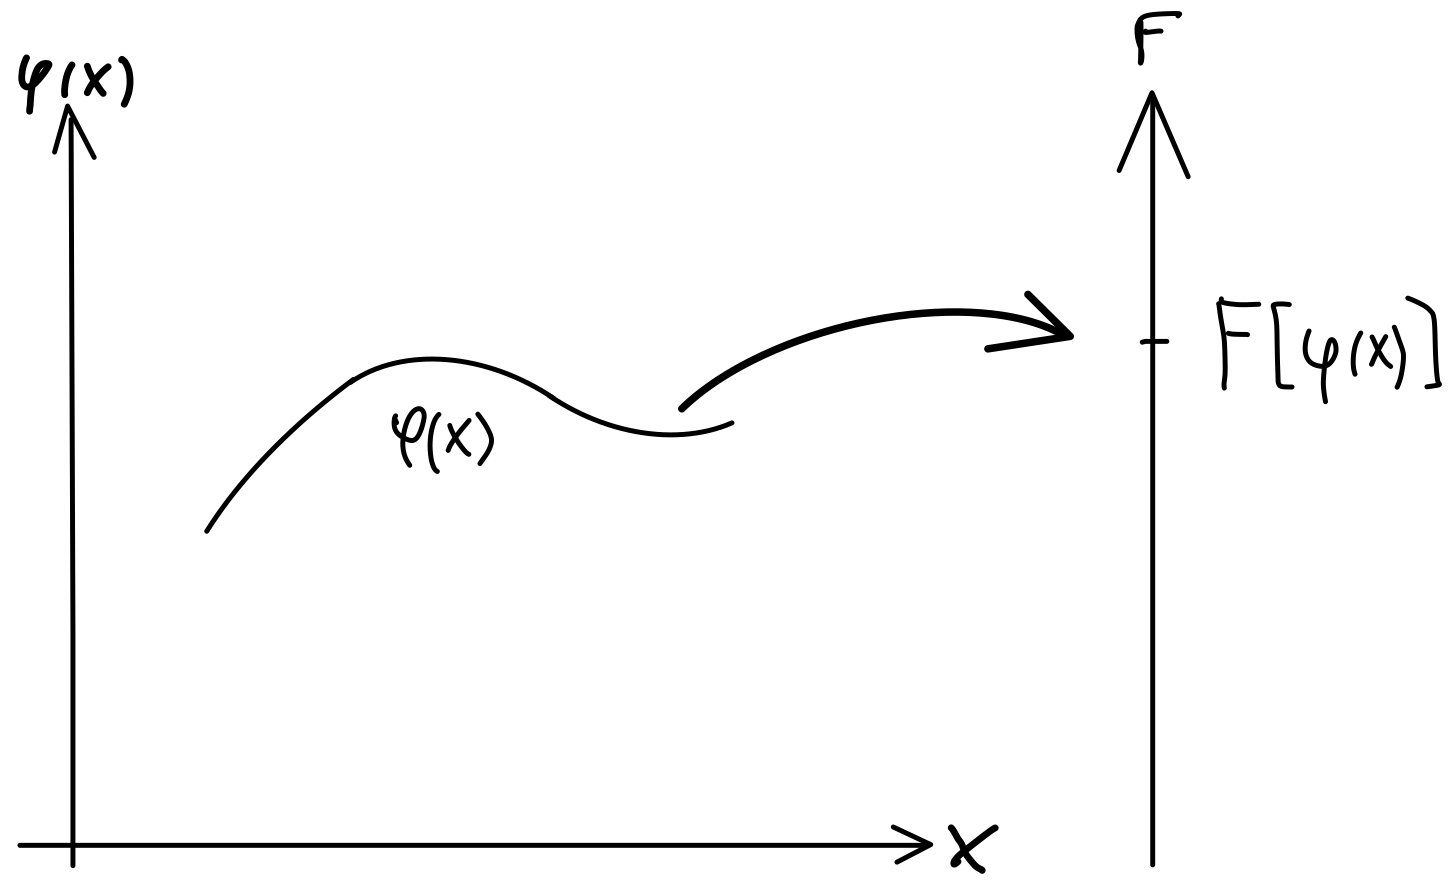
\includegraphics[width=0.4\textwidth]{fig/Funktional.png}
  \caption{Das Funktional der Funktion $\varphi(x)$. Man beachte, dass hiermit
  der gesamten Funktion $\varphi(x)$ ein Wert zugewiesen
  wird.\label{fig:functional}}
 \end{center}
\end{wrapfigure}
Gegeben eine Funktion $\varphi(x)$, dann nennen wir $F[\varphi(x)]$ ein
Funktional. Dies ist eine Erweiterung des Konzepts einer Funktion
$F(\varphi_1,\varphi_2,\dots)=F(\varphi_i)$ mehrerer Variabler, bei der wir den
diskreten Index $i$ durch eine kontinuierliche Variable $x$ ersetzen. Ein
Funktional ordnet also einer Funktion $\varphi(x)$ einen Wert zu. Wir stellen
uns das vor, wie in Abbildung \ref{fig:functional} skizziert.\\
\\
\\
\\
\\
\\
\\
\\
\\

\begin{example}{Verschiedene Beispiele von Funktionalen}
Ein Funktional kann repräsentiert sein durch
\begin{itemize}
\item 
$F[\varphi]=\int\limits_a^b\varphi(x)dx$, das Integral von $\varphi(x)$
  über einem Intervall $[a,b]$, oder
\item 
  $F[\varphi]=\int\limits_a^bf(\varphi(x))dx$, das Integral einer Funktion
  $f$ von $\varphi(x)$ auf dem Intervall $[a,b]$, oder
\item 
  $F[\varphi]=\int\limits_a^bf(\varphi(x), \varphi'(x))dx$, das Integral
  einer Funktion $f$ von $\varphi(x)$, die auch von der Ableitung $\varphi'(x)$
  abhängt, oder 
\item 
  $F[\varphi]=\varphi(y)=\int\limits_a^b\varphi(x)\delta(y-x)dx$, einem
  Integral dessen Integrand die Deltafunktion enthält, usw. 
\end{itemize}
  Eine Erweiterung auf mehrere Funktionen, die auch noch von mehreren Variablen
  abhängen können ist möglich $F[\varphi_i(x_k)]$. Dabei kann
  $F[\varphi_i(x_k)]$ auch ein Integral einer Funktion $f$ der $\varphi_i(x_k)$
  und deren verschiedenen partiellen Ableitungen sein.
\end{example}
\section{Exkurs zur Diracschen Deltafunktion}\label{sec:Deltafunktion}
Zunächst sei hier eine Warnung ausgesprochen. Deltafunktionen sind keine
Funktionen im eigentlichem Sinne, obwohl sie oftmals so bezeichnet werden. In
der Mathematik werden diese Objekte als Distributionen bezeichnet. Da ihre
Wirkung auf echte Funktionen von ihrer genauen Definition abhängt, ist
Vorsicht bei ihrer Anwendung geboten.
\subsection{Definition der Deltafunktion}
Wir beginnen mit einem Beispiel und legen die Folge von Glockenkurven
\begin{equation}\label{eq:Lorentzian}
y(x,\varepsilon)=\frac{1}{\pi}\frac{\varepsilon}{x^2+\varepsilon^2}
\end{equation}
zugrunde. Mit kleiner werdendem $\varepsilon$ werden diese Funktionen immer
schmaler und höher, wie man in Abbildung \ref{fig:Glockenkurven} sehen kann.

Im Limes $\varepsilon\rightarrow 0$ ist die Funktion gleich Null für $x\ne 0$
und für $x=0$ divergiert sie. Wir schreiben dies formal als
\[ \lim_{\varepsilon\rightarrow 0} y(x,\varepsilon)=
  \left\{\begin{matrix}0& x\ne 0\\\infty& x=0\end{matrix}\right.\]
Die unter den in (\ref{eq:Lorentzian}) definierten Kurven liegende Fläche ist
\[\int_{-\infty}^{\infty}\frac{1}{\pi}\frac{\varepsilon}{x^2+\varepsilon^2}dx=
  \left.\frac{1}{\pi}\arctan \frac{x}{\varepsilon}\right|_{-\infty}^{\infty}=1.\]
Diese ist unabhängig von $\varepsilon$ immer 1, wie wir sehen.

\begin{wrapfigure}[18]{l}{0.45\textwidth}
  \begin{center}
   \begin{tikzpicture}%[domain=0:4]
    \begin{axis}[domain=-3:3,
	xmin=-3.2, xmax=3.2,
	ymin=-.2, ymax=10.5,
        axis y line=center,
        axis x line=middle,
	style = thick,
	xticklabel style = { font = \small, anchor = north},
	xtick = {1},
	ytick={\empty},
	extra y ticks= {5,10},
	extra y tick labels = {5,10},
	extra y tick style = { font = \small, anchor = west},
        samples=400]
      \addplot+[mark=none] {1./(x^2+1.)};
      \addplot+[mark=none] {.2/(x^2+.04)};
      \addplot+[mark=none] {.1/(x^2+.01)};
    \end{axis}
   \end{tikzpicture}
  \end{center}
  \caption{\label{fig:Glockenkurven}Glockenkurven wie in (\ref{eq:Lorentzian})
  definiert, mit den $\varepsilon$-Werten 1. (blau), 0.2 (rot) und 0.1 (grün).}
\end{wrapfigure}
Gegeben eine stetige Funktion $f(x)$. Wir betrachten das Integral
\[I(\varepsilon)=\int_{-\infty}^{\infty}f(x)y(x,\varepsilon)dx\]
als Funktion von $\varepsilon$ und schreiben den Grenzübergang formal als
\begin{equation}\label{eq:intfy}
  \lim_{\varepsilon\rightarrow 0}\int_{-\infty}^{\infty}f(x)y(x,\varepsilon)dx=
\int_{-\infty}^{\infty}f(x)\delta(x)dx
\end{equation}

Die so definierte Deltafunktion ist ein Symbol und keine Funktion im Sinne der
Analysis. Wir sollten uns stets vor Augen halten, dass die Bildung des
Grenzwertes $\lim_{\varepsilon\rightarrow 0}$ mit der Integration über $x$
nicht vertauschbar ist, das heißt, dass vor der Limesbildung stets die
Integration auszuführen ist.\vspace{1cm}

Um den Grenzwert in (\ref{eq:intfy}) ausrechnen zu können machen wir die
Substitution $x=\varepsilon\xi$. Damit erhalten wir
\[ F(\varepsilon)=\int_{-\infty}^{\infty}f(\varepsilon\,\xi)
\frac{1}{\pi}\frac{1}{\xi^2+1}d\xi\]
Das Integral über die Glockenfunktion ist, wie wir bereits ausgerechnet haben,
gegeben als
\[\int_{-\infty}^{\infty}\frac{1}{\pi}\frac{1}{\xi^2+1}d\xi=1.\]
Damit können wir den Grenzübergang $\varepsilon\rightarrow 0$ in
$F(\varepsilon)$ unter dem Integral ausführen und erhalten
\[F(0)=\int_{-\infty}^{\infty}f(0)
\frac{1}{\pi}\frac{1}{\xi^2+1}d\xi=f(0)\]
\subsection{Eigenschaften der Deltafunktion}
Gegeben eine stetige Funktion $g(x)$ mit einfachen Nullstellen bei $x_n$, d.h.
$g(x_n)=0$ und $g'(x_n)\ne 0$, so gilt
\[\delta(g(x))=\sum\limits_n\frac{1}{|g'(x_n)|}\delta(x-x_n)\]

Bilden wir die Ableitung der Funktion $y(x,\varepsilon)$ nach $x$, so erhalten
wir von der Glockenkurve ausgehend 
\[y'(x,\varepsilon)=-\frac{2}{\pi}\frac{\varepsilon x}{(\varepsilon^2+x^2)^2}\]
Nun berechnen wir den Grenzübergang des Integrals
\begin{equation}\label{eq:deltaderivative}
\lim_{\varepsilon\rightarrow 0}\int_{-\infty}^{\infty}f(x)y'(x,\varepsilon)dx=
\underbrace{\left.\lim_{\varepsilon\rightarrow 0}f(x)y(x,\varepsilon)\right|_{-\infty}^{\infty}}_{0}
-\lim_{\varepsilon\rightarrow 0}\int_{-\infty}^{\infty}f'(x)\delta(x)dx
\end{equation}
In (\ref{eq:deltaderivative}) zeigt sich im ersten Term auf der rechten Seite
der Gleichung die erste Schwierigkeit. Damit dieser an den Grenzen
verschwindet, muss $y(x,\varepsilon)$ im Gernzübergang schneller gegen Null
gehen als $f(x)$. Daher die Warnung am Anfang des Abschnitts.

Wir erinnern uns an die Fourierintegrale (\ref{eq:fourierhin}, \ref{eq:fourierrueck})
\[
F(k)=\int_{-\infty}^{\infty}e^{-ikx}f(x)dx\\
f(x)=\frac{1}{2\pi}\int_{-\infty}^{\infty}e^{ikx}F(k)dk
\]
Setzen wir die erste in die zweite Zeile ein, dann erhalten wir
\[f(x)=\frac{1}{2\pi}\int_{-\infty}^{\infty}\int_{-\infty}^{\infty}e^{ik(x-x')}f(x')dx'dk\]
mit der Integration über $k$ nach der über $x'$. Wenn das Gleihheitszeichen
gelten soll, dann muss
\[\delta(x-x')="\frac{1}{2\pi}\int_{-\infty}^{\infty}e^{ik(x-x')}dk".\]
Wobei ``'' bedeutet, dass die Integration über $k$ erst nach der über $x'$
erfolgen soll. Dies ist die Fourierdarstellung der $\delta$-Funktion.
%
\section{Funktionalableitung oder Variation des Funktionals}\label{sec:Funktionalableitung}
Gegeben das Funktional $F[\varphi(x)]$. Wenn wir nun die Funktion $\varphi(x)$
ändern um einen Wert $\Delta\varphi$, dann ändert
sich auch das Funktional
$F[\varphi+\Delta\varphi]=F[\varphi]+\Delta F$. 

Um dies zu verstehen, variieren wir $\varphi(x)$ nur in einer endlichen
Umgebung $dx_0$ des Punktes $x_0$, also
$F[\varphi+\varepsilon(x_0,dx_0)\Delta\varphi]$, mit 
  \begin{equation}\label{eq:umgebungeps}
    \varepsilon(x_0,dx_0)=\left\{\begin{matrix}1\text{ für
    }x\in[x_0-\frac{dx_0}{2},x_0+\frac{dx_0}{2}]\\ 0 \text{
    sonst}\end{matrix}\right.
  \end{equation}
Damit schreiben wir $\Delta
F=F[\varphi+F[\varphi+\varepsilon(x_0,dx_0)\Delta\varphi]-F[\varphi]$. Dies
schreiben wir im Grenzübergang für verschwindende $\Delta\varphi$ und $dx_0$
als
\begin{equation}\label{eq:Variationsableitung}
  \lim_{dx_0\rightarrow 0}\lim_{\Delta\varphi\rightarrow 0}
      \frac{F[\varphi+\varepsilon(x_0,dx_0)\Delta\varphi]-F[\varphi]}{\Delta\varphi dx_0}
    =\frac{\delta F[\varphi]}{\delta\varphi(x_0)}
\end{equation} 
Diese Funktionalableitung oder Variation von $F$ ist die Varallgemeinerung der
partiellen Ableitung $\frac{\partial F[\varphi]}{\partial\varphi_k}$.
%
\begin{figure}[!h] 
 \begin{center}
  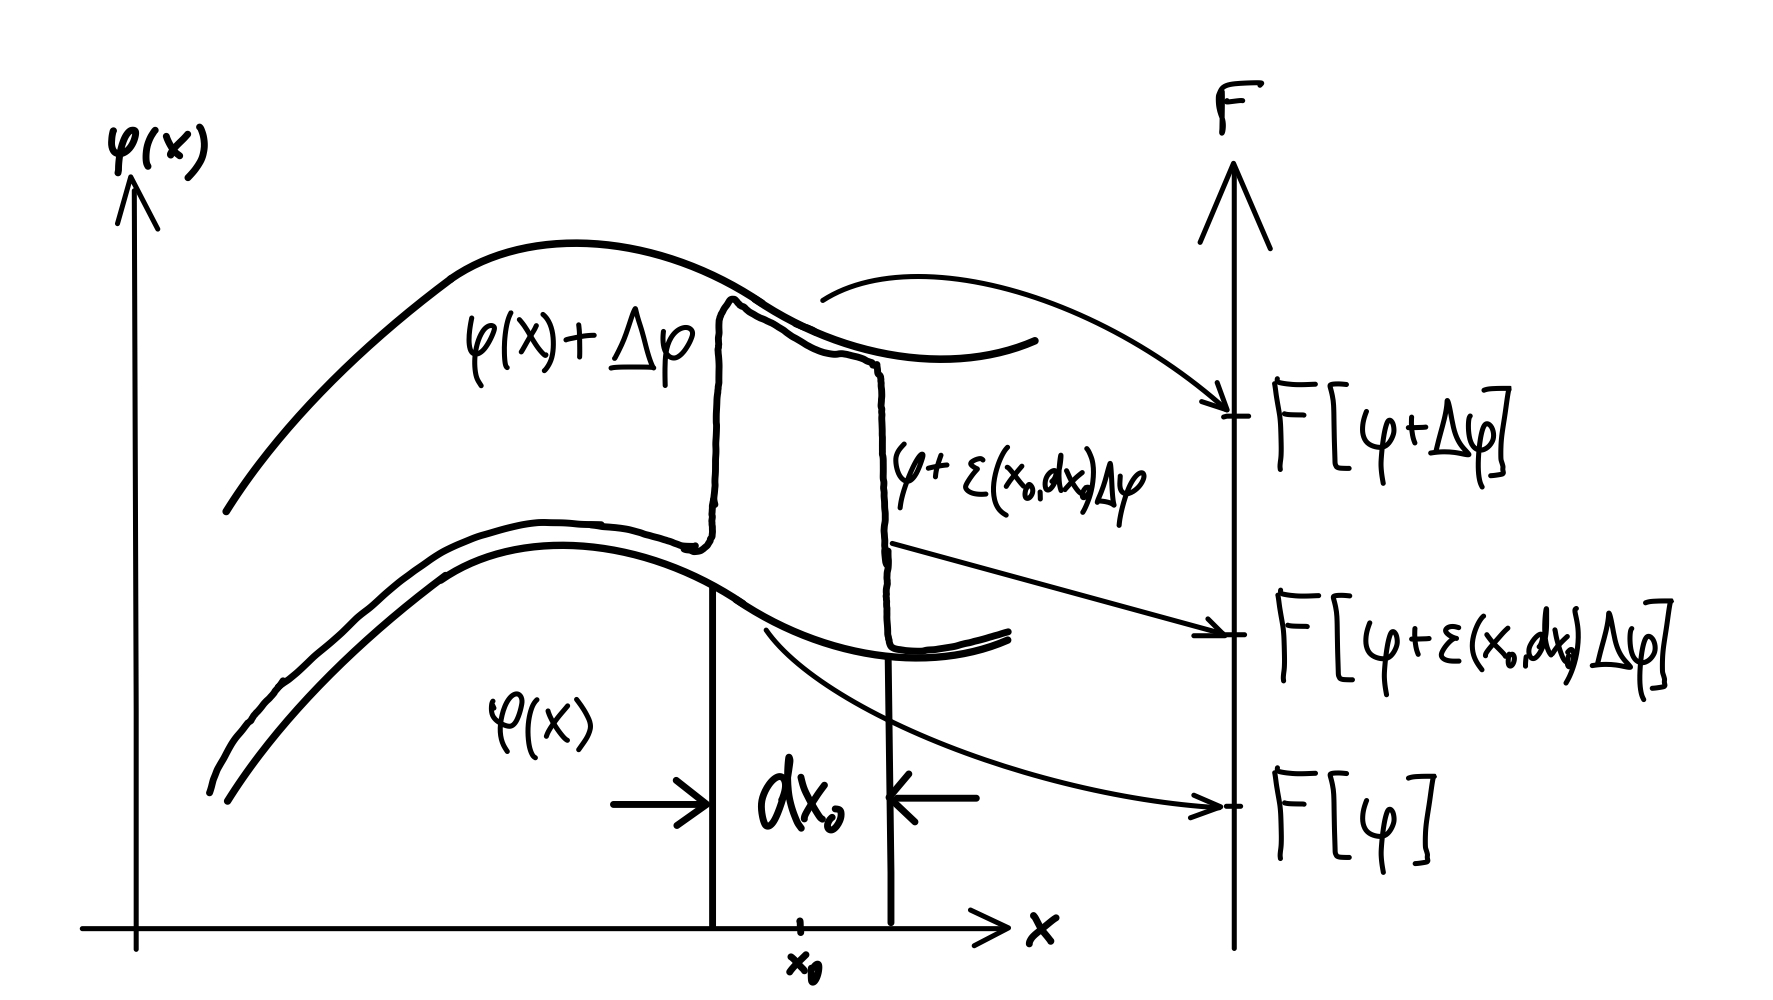
\includegraphics[height=0.4\textwidth]{fig/Variation.jpeg}
  \caption{Die Variation eines Funktionals der Funktion $\varphi(x)$. Wie
    ändert sich das Funktional, wenn die gesamte Funktion $\varphi(x)$ variiert
    wird? $F[\phi]$ ist der Wert den Funktionals,
    $F[\phi+\varepsilon(x_0,dx_0)\Delta\varphi]$ ist der Wert des Funktionals
    wenn wir in einer $\varepsilon$-Umgebung von $x_0$ die Funktion $\varphi$
    um $\Delta\varphi$ ändern. Somit ist die Änderung des Funktionals $\Delta
    F=F[\phi+\varepsilon(x_0,dx_0)\Delta\varphi]-F[\phi]$, wenn wir in einer
    $\varepsilon$-Umgebung von $x_0$ die Funktion $\varphi$ um $\Delta\varphi$
    ändern. Die gesamte Änderung ergibt sich nun durch das Integral über $\Delta
    F$.\label{fig:variation}}
 \end{center}
\end{figure}
%
Das Differential $\Delta F$ zu einer beliebigen differentiellen Veränderung
$\delta\varphi$ erhalten wir durch Integration über alle $x_0$
\begin{equation}\label{eq:DifferentialVariation}
  \Delta F = \int\frac{\delta F[\varphi]}{\delta\varphi(x_0)}\Delta\varphi(x_0)dx_0,
\end{equation}
wobei die entsprechende diskrete Version des Differentials, wie wir bereits
wissen, folgendermaßen definiert ist
\begin{equation}\label{eq:DifferentialMultiD}
    \Delta F = \sum\limits_k \frac{\partial F[\varphi_k]}{\partial\varphi_k}\Delta\varphi_k
\end{equation}
%
\subsection{Liste wichtiger Funktionalableitungen}\label{sec:WichtigeAbleitungen}
\begin{itemize}
  \item Sei $F[\varphi]=\varphi(\tilde{x})$ dann erhalten wir
    \[
      \frac{\delta\varphi(\tilde{x})}{\delta\varphi(x)}=\lim_{dx_0\rightarrow 0}\lim_{\Delta\varphi\rightarrow 0}
      \frac{\varphi(\tilde{x})+\varepsilon(\tilde{x},x,dx_0)\Delta\varphi-\varphi(\tilde{x})}{\Delta\varphi dx_0}=\lim_{dx_0\rightarrow 0}\frac{\varepsilon(\tilde{x},x,dx_0)}{dx_0}=\delta(\tilde{x}-x)
    \]
  \item Mit der obigen Überlegung und $F[\varphi]=\varphi'(\tilde{x})$ erhalten wir analog
    \[
      \frac{\delta\varphi'(\tilde{x})}{\delta\varphi(x)}=\frac{d}{d\tilde{x}} \frac{\delta\varphi(\tilde{x})}{\delta\varphi(x)}=\frac{d}{d\tilde{x}}\delta(\tilde{x}-x)=-\frac{d}{dx}\delta(\tilde{x}-x)
    \]
    wobei hier wieder Vorsicht geboten ist mit der Wirkung der Ableitung einer
    Deltafunktion (siehe Abschnitt \ref{sec:Deltafunktion}).
  \item Für $F[\varphi]=f(\varphi(\tilde{x}))$ erhalten wir mit Hilfe der Kettenregel
    \[
      \frac{\delta f(\varphi(\tilde{x}))}{\delta\varphi(x)}=\frac{df}{d\varphi}\delta(\tilde{x}-x).
    \]
    Deshalb haben wir im Fall  $F[\varphi]=f(\varphi(\tilde{x}),\varphi'(\tilde{x}))$
      \[
	\frac{\delta f(\varphi(\tilde{x}),\varphi'(\tilde{x}))}{\delta\varphi(x)}=
	\frac{\partial f(\varphi(\tilde{x}),\varphi'(\tilde{x})}{\partial\varphi(\tilde{x})}\delta(\tilde{x}-x)-
	  \frac{\partial f(\varphi(\tilde{x}),\varphi'(\tilde{x})}{\partial\varphi'(\tilde{x})}\frac{d}{dx}\delta(\tilde{x}-x).
    \]
  \item Setzen wir $F[\varphi]=\int f(\varphi(\tilde{x}))d\tilde{x}$ dann erhalten  wir 
    \[
      \frac{\delta F[\varphi]}{\delta\varphi(x)}=\int \frac{\partial f(\varphi(\tilde{x}))}{\partial\varphi(x)}d\tilde{x}=
      \int\frac{\partial f(\varphi(\tilde{x}))}{\partial\varphi(\tilde{x})}\frac{\partial\varphi(\tilde{x})}{\partial\varphi(x)}d\tilde{x}=
      \int\frac{\partial f(\varphi(\tilde{x}))}{\partial\varphi(\tilde{x})}\delta(\tilde{x}-x)d\tilde{x}=\frac{\partial f}{\partial\varphi}
    \]
\end{itemize}

Wir wenden die obigen Fälle auf das Funktional $F[\varphi]=\int
f(\varphi(\tilde{x}),\varphi'(\tilde{x}))d\tilde{x}$ an und erhalten
 \[
   \frac{\delta F[\varphi]}{\delta\varphi(x)}=\int \frac{\delta f(\varphi(\tilde{x}),\varphi'(\tilde{x}))}{\delta\varphi(x)}d\tilde{x}=
   \int\left(\frac{\partial f(\varphi(\tilde{x}),\varphi'(\tilde{x}))}{\partial\varphi(\tilde{x}))}\delta(\tilde{x}-x)-
 \frac{\partial f(\varphi(\tilde{x}),\varphi'(\tilde{x}))}{\partial\varphi'(\tilde{x})}\frac{d}{dx}\delta(\tilde{x}-x)\right)d\tilde{x}.
    \]
Die Ableitung nach „x“ unter dem Integral können wir vor das Produkt ziehen, so dass wir
\[
   \frac{\delta F[\varphi]}{\delta\varphi(x)}=\int \frac{\delta f(\varphi(\tilde{x}),\varphi'(\tilde{x}))}{\delta\varphi(x)}d\tilde{x}=
   \int\left(\frac{\partial f(\varphi(\tilde{x}),\varphi'(\tilde{x}))}{\partial\varphi(\tilde{x})}-\frac{d}{dx}
       \frac{\partial f(\varphi(\tilde{x}),\varphi'(\tilde{x}))}{\partial\varphi'(\tilde{x})}\right)\delta(\tilde{x}-x)d\tilde{x}.
\]
erhalten. Nach dem Ausführen der Integration bleibt
\[
  \frac{\delta F[\varphi]}{\delta\varphi(x)}=\frac{\partial f(\varphi(x),\varphi'(x))}{\partial\varphi(x)}
  -\frac{d}{dx} \frac{\partial f(\varphi(x),\varphi'(x))}{\partial\varphi'(x)}
\]
 Dies ist ein wichtiges Ergebnis, das wir im folgenden genauer betrachten
 wollen.
%
\subsection{Das Extremalprinzip in der Mechanik}
Gegeben sei eine Funktion $L(q(t),\dot q(t))$. Wir stellen uns die Frage für
welche Funktion $q(t)$ das Funktional
\[
  S[q(t)]=\int_a^b L(q(t),\dot q(t)) dt
\]
extremal wird. D.h. wir suchen unter allen möglichen Funktionen $q(t)$
diejenige, die $S[q(t)]$ extremal werden lässt. Oder in anderen Worten, wir
wollen dasjenige $q(t)$ finden, für das jegliche Variation von $S[q(t)]$
verschwindet, also 
\[\frac{\delta S[q]}{\delta q}=0\]
Diese Variation haben wir aber bereits im vorigen Abschnitt als Beispiel angegeben
\[
  \frac{\delta S[q]}{\delta q}=\frac{\partial L(q(t),\dot q(t)}{\partial q(t)}
    -\frac{d}{dt} \frac{\partial L(q(t),\dot q(t))}{\partial \dot q(t)}=0
\]
\begin{note}{Der harmonische Oszillator}
Wir setzen $L(q(t),\dot q(t))=\frac{1}{2}m\dot
q(t)^2-\frac{1}{2}k q(t)^2$ und erhalten
\[ \frac{\partial L(q(t),\dot q(t)}{\partial q(t)}
    -\frac{d}{dt} \frac{\partial L(q(t),\dot q(t))}{\partial \dot q(t)}=
   -kq(t)-\frac{d}{dt}m\dot q(t)
   =0.
 \]
 Dies ist die wohlbekannte Bewegungsgleichung des harmonischen Oszillators\newline 
 \[m\ddot q(t)+kq(t)=0.\]

Hieraus folgern wir, ohne dass wir hier den Beweis antreten, dass die
Lagrangefunktion $L=T^*-V$ eines mechanischen Systems aus der Differenz
ziwschen kinetischer Koenergie\footnote{Die Unterscheidung zwischen kinetischer
  Energie $T=\frac{p^2}{2m}$ und kinetischer Koenergie $T=\frac{mv^2}{2}$ ist
  nur wichtig im Falle, dass der Impuls nicht mehr als $p=m\cdot v$ geschrieben
werden kann. Dies ist z.B. der Fall, wenn relativistische Effekte wichtig
werden. Wir nehmen an, dass dies im Folgenden nicht der Fall sei und machen
fortan diese Unterscheidung nicht.} 
%
und potentieller Energie gebildet wird. Indem wir fordern, dass die
Variation des Integrals über die Lagrangefunktion verschwindet, erhalten wir
die Bewergungsgleichungen, der entsprechenden mechanischen Systeme. Diese
Gleichungen nennen wir die Euler-Lagrange-Gleichungen.
\end{note}
Wir fügen ein Beispiel allgemeinerer Natur an.
\begin{example}{Das Brachistochronenproblem}
  \begin{wrapfigure}{l}{0.5\textwidth}
  \centering
  \begin{tikzpicture}[scale=0.8]
    \begin{axis}[domain=0:4.0, xmin=0, xmax=3.8, ymin=0, ymax=5, axis y line = left,
     axis x line = bottom, axis line style = {-latex}, 
     xticklabel style = { font = \small, anchor = north}, xtick = {\empty}, ytick = {\empty},
     xlabel style={at={(rel axis cs:1.05,.15)}}, xlabel=$x$,
     ylabel style={at={(rel axis cs:0.2,1.05)},rotate=-90}, ylabel=$y$,
     extra x ticks = {3.8},
     extra x tick labels = {$x_0$},
     extra y ticks = {4.5},
     extra y tick labels = {$y_0$},
     extra y tick style = { font = \small, anchor = west},
     samples=400]
     \addplot+[mark=none] {4.5*((x-3.8)^2)/14.44};
     \addplot+[mark=none] {4.5*((x-3.8)^2)/14.44+0.2*sin(x*47.37)-.2*sin(3*x*47.37)-.15*sin(4*x*47.37)};
    \end{axis}
   \end{tikzpicture}
   \caption{Verschiedene Notrutschen.}
  \label{fig:Rutsche}
 \end{wrapfigure}
  Unsere Aufgabe sei es, eine Notrutsche für die Evakuierung eines Flugzeugs zu
  konstruieren. Die Rutsche soll eine solche Form haben, dass die Passagiere
  darauf auf dem schnellsten Weg den Boden erreichen.  Die Situation ist in
  \ref{fig:Rutsche} schematisch dargestellt. Die Passagiere steigen bei $x=0$
  auf die Rutsche in einer Höhe von $y=y_0$ und rutschen zum Punkt $x=x_0$ bei
  $y=0$.

  Hier ist eine Funktion $y(x)$ gesucht, die eine Bedingung erfüllen muss, die
  wir nun formulieren wollen. Wir gehen von Energieerhaltung aus, d.h. die
  Lageenergie am Einstiegspunkt wird bis zum momentanen Punkt auf der Rutsche
  in kinetische Energie umgewandelt, oder 
  \[ mgy_0=\frac{1}{2}m(\dot{y}^2+\dot{x}^2)+mgy \]
  oder
  \begin{equation}
  g(y_0-y)=\frac{1}{2}\left[\left(\frac{dx}{dt}\right)^2
    +\left(\frac{dy}{dt}\right)^2\right]
    \label{eq:Rutschenergie}
  \end{equation}
  Wie wir sehen, kürzt sich die Masse raus. D.h. schwere und leichte Passagiere
 rutschen gleich schnell. Ist das Modell vollständig?
 
 Wir schreiben (\ref{eq:Rutschenergie}) um
 \begin{equation}
   (dt)^2=\frac{(dx)^2+(dy)^2}{2g(y_0-y)}
   \label{eq:RutscheAufgeloest}
 \end{equation}
 (\ref{eq:RutscheAufgeloest}) kann nun benutzt werden um die Zeit $T$ zu berechnen,
 die es braucht um auf einer gegebenen Funktion $y(x)$ von $(0,y_0)$ nach
 $(x_0,0)$ zu rutschen. Die Zeit $T$ ist ein Funktional
 \begin{equation}
    T[y]=\int\limits_{0}^{x_0}\sqrt{\frac{1+\left(\frac{dy}{dx}\right)^2}{2g(y_0-y)}}dx
    =\int\limits_{0}^{x_0}\sqrt{\frac{1+y'(x)}{2g(y_0-y(x))}}dx
    =\int\limits_{0}^{x_0}f(y(x),y'(x))dx=F[y]
   \label{eq:Zeitfunktional}
 \end{equation}
 Damit habe wir das Variationsproblem $\frac{\delta T[y]}{\delta y}=0$ zu
 lösen. Aus der obigen Liste der wichtigsten Funktionalableitungen in
 Abschnitt \ref{sec:WichtigeAbleitungen} sehen wir, dass wir die Euler-Lagrange
 Gleichungen
 \[ 
   \frac{\partial f(y(x),y'(x))}{\partial y(x)}
    -\frac{d}{dx} \frac{\partial f(y(x),y'(x)}{\partial y'(x)}=0
 \]
 benutzen können und bekommen damit eine Differentialgleichung zur Bestimmung
 von $y(x)$.
\end{example}
%
\subsection{Variation von Mehrfachintegralen}
Wir erweitern den Begriff des Funktionals, wie wir ihn in Abschnitt
\ref{sec:DasFunktional} definierten, indem wir anstatt des Integrals der
Funktion $L(q(t),\dot q(t))$ nun ein Funktional betrachten, das aus einem
Mehrfachintegral besteht. Dafür setzen wir anstatt der Funktion $q(t)$, das
Feld $\varphi(x_{\mu})$ in $L$ ein und schreiben die Funktion $L$ von nun an
als $\mathcal{L}$. Hierbei bezeichne $x_{\mu}$ die $\mu$-te unabhängige
Variable. Ausserdem erweitern wir die in $\mathcal{L}$ vorhandenen Ableitungen
auf die partiellen Ableitungen erster und höherer Ordnung der Funktion
$\varphi(\mathbf{x})$. Damit ist $\mathcal{L}$ eine Funktion 
\begin{equation}\label{eq:LagrangeDensity}
  \mathcal{L}=\mathcal{L}\left(\varphi(x_\mu),\frac{\partial\varphi(x_\mu)}{\partial x_{\nu}},
  \frac{\partial^2\varphi(x_\mu)}{\partial x_{\nu}\partial x_{\kappa}}\dots ;\, x_\mu\right)
\end{equation}
und wir haben ein mehrdimensionales Variationsproblem vorliegen. Das Funktional
sei gegeben als n-dimensionales Integral
\begin{equation}\label{eq:nDFunktional}
  J[\varphi]=\int\limits_{\Omega}\mathcal{L}\left(
    \varphi(x_\mu),\partial_{\nu}\varphi(x_\mu),
    \partial_{\nu\kappa}\varphi(x_\mu)\dots ;\, x_\mu\right)d^nx_\mu
\end{equation}
wobei wir für $\frac{\partial}{\partial x_{\nu}}=\partial_{\nu}$,
$\frac{\partial^2}{\partial x_{\mu}\partial x_{\nu}} =\partial_{\mu\nu}$
geschrieben haben. Variieren wir nun die Funktion $\varphi(x_\mu)$ um einen
Wert $\psi(x_\mu)$, wie bereits in Abschnitt \ref{sec:Funktionalableitung}
beschrieben, dann erhalten wir für die Variation des Integrals in
(\ref{eq:nDFunktional})
\begin{align} \label{eq:VariationFeld}
  \delta J[\varphi]=& J[\varphi+\varepsilon\psi]-J[\varphi]=\\
  =&\int\limits_{\Omega}\Bigl[\mathcal{L}(
    \varphi(x_\mu)+\varepsilon\psi(x_\mu),
      \partial_{\nu}\varphi(x_\mu)+\varepsilon\partial_{\nu}\psi(x_\mu),
      \partial_{\nu\kappa}\varphi(x_\mu)+\varepsilon\partial_{\nu\kappa}\psi(x_\mu)\dots ;\, x_\mu)\nonumber\\
      &-\mathcal{L}( \varphi(x_\mu),\partial_{\nu}\varphi(x_\mu),
     \partial_{\nu\kappa}\varphi(x_\mu)\dots ;\, x_\mu)\Bigr]d^n x_\mu \nonumber
\end{align}
Wir entwickeln (\ref{eq:VariationFeld}) in eine Potenzreihe nach $\varepsilon$
und behalten alle Glieder bis zur ersten Ordnung, dann erhalten wir
\begin{equation}\label{eq:VariationTaylor1}
  \delta J[\varphi]=\varepsilon\int\limits_{\Omega}\Bigl(
    \frac{\partial\mathcal{L}}{\partial\varphi}\psi
    +\frac{\partial\mathcal{L}}{\partial(\partial_{\mu}\varphi)}\partial_{\mu}\psi
  +\frac{\partial\mathcal{L}}{\partial(\partial_{\mu\nu}\varphi)}\partial_{\mu\nu}\psi+\cdots\Bigr)d^n x_\mu
\end{equation}
Wir wählen $\psi$ dergestalt, dass es auf dem Rand des Integrationsgebietes
verschwindet, also $\psi(x_{\mu}\in\Omega)=0$, dann erhalten wir durch
partielle Inegration von (\ref{eq:VariationTaylor1})
\begin{equation}\label{eq:VariationFunktionalFeld}
 \delta J[\varphi]=\varepsilon\int\limits_{\Omega}\left(
    \frac{\partial\mathcal{L}}{\partial\varphi}
    -\partial_{\mu}\frac{\partial\mathcal{L}}{\partial(\partial_{\mu}\varphi)}
    +\partial_{\mu\nu}\frac{\partial\mathcal{L}}{\partial(\partial_{\mu\nu}\varphi)}
  -\cdots\right)\psi\, d^n x_\mu
\end{equation}
Für beliebige $\psi$ folgen daraus die Bewegungsgleichungen für das Feld $\varphi(x_\mu)$ zu
\begin{equation}
  \frac{\partial\mathcal{L}}{\partial\varphi}
  -\partial_{\mu}\frac{\partial\mathcal{L}}{\partial(\partial_{\mu}\varphi)}
  +\partial_{\mu\nu}\frac{\partial\mathcal{L}}{\partial(\partial_{\mu\nu}\varphi)}
  -\partial_{\mu\nu\gamma}\frac{\partial\mathcal{L}}{\partial(\partial_{\mu\nu\gamma}\varphi)}
  \cdots=0
  \label{eq:EulerLagrangeFeld}
\end{equation}
\subsection{Die schwingende Saite, ein ausführliches Beispiel}
\begin{tikzpicture} %[domain=0:4]
    \begin{axis}[%width=\textwidth,height=0.5\textwidth, 
	width=16cm,
	height=8cm,
        hide x axis,
        hide y axis,
        samples=400]
	\addplot+[domain=0:180,mark=none,ultra thick] {(cos(x))};
	\draw[thick,decoration={aspect=0.41, segment length=2.3mm, 
	amplitude=2.2mm,coil},decorate] (0.0,200.0) -- (0.0,100.0);
	\node at (10,150) {$k$};
	\node at (170,50) {$k$};
	\draw[thick,decoration={aspect=0.41, segment length=2.3mm, 
	amplitude=2.2mm,coil},decorate] (180,0.0) -- (180,100.0);
	\draw[-Latex,thick] (-10,-20) -- (-10,200);
	\node[above] at (-10,200) {u};
	\draw[-Latex,thick] (-10,100) -- (190,100);
	\node[right] at (190,100) {x};
	\draw[thick, dashed] (0,100) -- (0,200);
	\draw[thick, dashed] (180,0) -- (180,100);
	\node at (10,80) {$x=0$};
	\node at (170,120) {$x=\ell$};
	\draw[thick] (130,100) -- (130,95);
	\draw[thick] (150,100) -- (150,95);
	\node [above] at (140,40) {$\Delta x$};
	\node [right] at (150,25) {$\Delta u$};
	\node [left] at (145,15) {$\sqrt{\Delta x^2+\Delta u^2}=\Delta s$};
	\addplot+[domain=130:150,mark=none,ultra thick] {(cos(130))};
	\addplot[color=red,mark=none,ultra thick] coordinates { (150,{cos(130)}) (150,{cos(150)}) };
	\addplot[color=red,mark=none,ultra thick] coordinates { (130,{cos(130)}) (150,{cos(150)}) };
    \end{axis}
   \end{tikzpicture}

Eine Seite der Länge $\ell$ sei bei $x=0$ und $x=\ell$ jeweils über eine Feder
elastisch aufgehängt. Die Aufhängepunkte sollen sich nur senkrecht zur
x-Richtung bewegen können (siehe Zeichung). Die Saite habe eine Massendichte
$\rho$ pro Längeneinheit und eine Spannung $\tau$. Die Federn der Aufhängung
haben eine Fedekonstante $k$.
   
Die kinetische Energie eines Abschnitts $\Delta x$ der Saite ist 
\[
  \Delta T^*=\frac{1}{2}\Delta m\cdot v^2 =
  \frac{1}{2}\rho\Delta x\left(\frac{\partial
  u(x,t)}{\partial t}\right)^2,
\] 
wobei wir kleine Relativauslenkungen $\Delta u$ angenommen haben. Die gesamte
kinetische Energie ist die Summer aller Beiträge der Abschnitte $\Delta x$. Im
Grenzübergang $\Delta x\rightarrow 0$ wird hieraus ein Integral 
\begin{equation}\label{eq:Ekin}
  T^*=\frac{1}{2}\rho\int_0^\ell\left(\frac{\partial
  U(x,t)}{\partial t}\right)^2dx
\end{equation}

Dasselbe machen wir nun mit der potentiellen Energie. Aus der Grafik erkennen
wir, dass die elastische Energie gleich der Saitenspannung $\tau$ multipliziert
mit der Steckung $\Delta x$ ist. Ohne auslenkung können wir so die gesamte
elastische Energie ausrechnen. Wenn aber lokal eine Verschiebung $\Delta u$
vorliegt, dann wir die Saite gedehn auf die neue Länge $\sqrt{\Delta x^2+\Delta
u^2}=\Delta s$. Die elastische Energie, die die Saite zusätlich durch die
Dehnung aufnimmt ist gerade die Differenz $\Delta V=\tau\cdot(\sqrt{\Delta
x^2+\Delta u^2}-\Delta x)$. Dies können wir auch schreiben als $\Delta
V=\tau\cdot\left(\sqrt{1+\left(\frac{\Delta u}{\Delta
x}\right)^2}-1\right)\Delta x$. Für klein Dehnungen $\left(\frac{\Delta u}{\Delta
x}\right)$ entwickeln wir den Term unter der Wurzel und erhalten näherungsweise
\[
  V=\tau\cdot\left(1+\left(\frac{\Delta u}{\Delta x}\right)^2-1\right)\Delta x
  =\tau\cdot\left(\frac{\Delta u}{\Delta x}\right)^2\Delta x
\]
Im Grenzübergang wird hieraus
\begin{equation}
  V=\frac{1}{2}\tau\int_0^\ell\left(\frac{\partial u}{\partial x}\right)^2dx.
  \label{eq:Epot}
\end{equation}
Wir müssen noch die zwei potentiellen Energieterme an den Aufhängepunkten
berücksichtigen, diese sind
\begin{equation}
  V_k=\frac{1}{2}k\cdot u(0,t)^2 +\frac{1}{2}k\cdot u(\ell,t)^2.
  \label{eq:EpotSprings}
\end{equation}
Damit erhalten wir folgende Lagrangefunktion
\begin{equation}
  L=\int_0^\ell\left[
    \frac{\rho}{2}\left(\frac{\partial u(x,t)}{\partial t}\right)^2
   -\frac{\tau}{2}\left(\frac{\partial u(x,t)}{\partial x}\right)^2
 \right]dx-\frac{1}{2}k\left(u(0,t)^2 + u(\ell,t)^2\right).
  \label{eq:LagrangianSaite}
\end{equation}

Das Funktional $J[u]=\int_{t_0}^{t_1}L(u(x,t))dt$ nennen wir das
Wirkungsintegral. Wir berechnen die Variation des Wirkungsintegrals
\begin{flalign}\label{eq:VariationAction}
  \delta &J[u]=J[u+\varepsilon\psi]-J[u]\\
  &=\varepsilon\int_{t_0}^{t_1}\left\{\int_0^\ell\left[
    \rho\frac{\partial u(x,t)}{\partial t}\frac{\partial\psi(x,t)}{\partial t}
  -\tau\frac{\partial u(x,t)}{\partial x}\frac{\partial\psi(x,t)}{\partial x}
   \right]dx
 - k\left[u(0,t)\psi(0,t)+u(\ell,t)\psi(\ell,t)\right]\right\}dt\nonumber\\
  &=\varepsilon\int_{t_0}^{t_1}\int_0^\ell\left[
    -\rho\frac{\partial^2u(x,t)}{\partial t^2}
 +\tau\frac{\partial^2u(x,t)}{\partial x^2}\right]\psi(x,t)dxdt
 -\varepsilon\int_0^\ell k\left[u(0,t)\psi(0,t)+u(\ell,t)\psi(\ell,t)\right]dt\nonumber\\
 &+\varepsilon\int_{t_0}^{t_1}\tau\left[\frac{\partial u(\ell,t)}{\partial x}\psi(\ell,t)-
 \frac{\partial u(0,t)}{\partial x}\psi(0,t)\right]dt
 +\varepsilon\int_0^\ell\rho\left[\frac{\partial u(x,t_0)}{\partial t}\psi(x,t_0)-
   \frac{\partial u(x,t)}{\partial t}\psi(x,t_1)\right]dx\nonumber
\end{flalign}
Assume that for $t=t_0$ and $t=t_1$ we do not vary the path $u$, so the last
term in (\ref{eq:VariationAction}) vanishes and therefore we get to first order
in $\varepsilon$
\begin{align}\label{eq:VariationActionFinal}
\delta &J[u]=\varepsilon\int_{t_0}^{t_1}\int_0^\ell\left[
    -\rho\frac{\partial^2u(x,t)}{\partial t^2}
 +\tau\frac{\partial^2u(x,t)}{\partial x^2}\right]\psi(x,t)dxdt\nonumber\\
 &-\int_{t_0}^{t_1}\left(\tau\frac{\partial u(0,t)}{\partial x}+ku(0,t)\right)\psi(0,t)dt
 -\int_{t_0}^{t_1}\left(-\tau\frac{\partial u(\ell,t)}{\partial x}+ku(\ell,t)\right)\psi(\ell,t)dt
\end{align}
$J[u]$ nimmt ein Extermum an, wenn $\delta J[u]=0$ gilt und zwar für beliebige
Variationen $\psi(x,t)$ des Pfades $u(x,t)$. Also setzen wir zunächst einmal
eine Variation mit $\psi(0,t)=\psi(\ell,t)=0$ an. Dies führt auf die Bewegungsgleichung
\begin{equation}
   -\rho\frac{\partial^2u(x,t)}{\partial t^2}
 +\tau\frac{\partial^2u(x,t)}{\partial x^2}=0
  \label{eq:MotionString}
\end{equation}
Wenn $u(x,t)$ (\ref{eq:MotionString}) genügt, dann ist der erste Term in
(\ref{eq:VariationActionFinal}) immer null. Setzen wir abwechselnd
$\psi(0,t)=0$ und $\psi(\ell,t)\ne 0$ und umgekehrt, dann erhalten wir zwei
zusätzliche Gleichungen
\begin{align}
  \tau\frac{\partial u(0,t)}{\partial x}+ku(0,t)&=0\label{eq:BCStringLeft}\\
  \tau\frac{\partial u(\ell,t)}{\partial x}+ku(\ell,t)&=0\label{eq:BCStringRight}
\end{align}
(\ref{eq:BCStringLeft}) und (\ref{eq:BCStringRight}) sind die zu
(\ref{eq:MotionString}) gehörigen Randbedingungen. Diese Beispiel zeigt, wie
mit Hilfe der Variationsrechnung die Bewegungsgleichungen für ein System
ageleitet werden kann.
%\chapter{Interpolation und Integration}
%{\bf Learning goals:}
%\begin{itemize}
%\item Represent discrete data as functions to obtain function values apart from
%	the support points
%\item Increase presision at lower cost, i.e. few parameters together with
%	interpolating functions cover the whole space
%\item Fast numerical integration by using interpolated representations of
%	functions with a limited number of interpolating functions.
%\end{itemize}\newpage
\section{Diskrete Daten und Interpolationsfunktionen}
\subsection{Das Newton Polynom}\label{subsec:newton}
Gegeben eine funktion $f(x)$, die an einer endlichen Zahl von Punkten $x_i$ bekannt sei.
Wir haben $f(x_i)=y_i$.  Es seien $n+1$ Paare $P_i=(x_i,y_i)$ von Werten gegeben, die Stützstellen
Wir wollen uns eine pllynomiale Funktion n-ter Ordnung beschaffen, geschrieben als
\[p_n(x)=a_0+a_1 x+\dots +a_n x^n\]
für die
\[p_n(x_i)=a_0+a_1 x_i+\dots +a_n x_i^n=y_i\]
gilt. Das Newton'sche polynomoiale Approximationsschema ist das meistbenutzte,
da es unter anderem auch für irregulär verteilte Stützstellen funktioniert.
Darüberhinaus muss der Polynomgrad nicht a priori festgelegt werden.
\subsubsection{Dividierte Differenzen}
Dividierte Differenzen sind durch eine rekursive Division definiert. Sie sind sein nützliches Werkzeug, um die Koeffizienten von Interpolationspolynomen zu berechnen.
Für jede geordnete Folge von Stützstellen 
$x_k$, mit $k=0,1,\dots,n$ ist der Algorithmus zur Berechnung der dividierten Differenzen für eine Untermenge der Stützstellen gegeben als
\begin{eqnarray}
	\label{eq:divdiffs}
   D[x_i] f&=& f(x_i)=f_i, \qquad \nu \in \{ 0,\ldots,n\}\\
   D[x_i,x_j] f&=& \frac{f_j-f_i}{x_j-x_i}\nonumber\\
   D[x_i,x_j,x_k] f&=& \frac{D[x_j,x_k]f-D[x_i,x_j]f}{x_k-x_i}\nonumber\\
   D[x_i,x_j,\ldots,x_l,x_m] f&=& \frac{D[x_j,\dots,x_m]f-D[x_i,\dots,x_l]f}{x_m-x_i}\nonumber
\end{eqnarray} 
Manchmal ist ed bequemer die folgende Matrixnotation zu benutzen
\begin{equation} 
	D_{i,j}=D[x_i,x_{i+1},\dots,x_{i+j}]f
	\label{eq:invdivdiffs}
\end{equation}
\subsubsection{Berechnung der Newton'schen Form}
Wir wollen $f(x)\approx p_n(x)$ finden, wobei $p_n(x)$ ein Newton'sches Polynom
ist, gegeben durch die Punkte $(x_0,f_0),\dots,(x_n,f_n)$, das folgendermaßen
definiert sei
\begin{equation}
	p_n(x)=f_0+(x-x_0)D[x_0,x_1]f+\dots +(x-x_0)\cdots (x-x_{n-1})D[x_0,\dots,x_n]f
	\label{eq:newtonpoly}
\end{equation}
oder mit der oben erwähnten Matrixform der dividierten Differenzen
\[
p_n(x)=D_{0,0}+D_{0,1}(x-x_0)+\dots +D_{0,n}(x-x_0)\cdot(x-x_{n-1})=D_{0,0}+\sum_{k=1}^nD_{0,k}\prod_{j=0}^{k-1}(x-x_j)
\]
Der größte Vorteil der hier präsentierten Methode ist, dass die dividierten Differenzen 
$D_{i,k}$ eng mit der k-ten Ableitung am Punkt $i$ verbunden sind.  Es ist
hiermit möglich zu entscheiden, ob eine Funktion, die durch ein Anzahl von
Stützstellen gegeben ist,  durch ein Polynom k-terOrdnung approximierbar ist.  Anders
gesagt, wenn alle Koeffizienten der  Matrixform der dividierten Differenzen in
der k-ten Spalte von derselben Größenordnung sind, d.h.  $D_{0,k}\approx
D_{0,1}\approx D_{0,2}\approx\dots$.
\subsection{Lagrangeinterpolation}
Lagrangepolynome sind so konstruiert, dass Sie durch alle Stützstellenpunkte, wie in \ref{subsec:newton}, gehen.
\[
L_i(x)=\prod_{j=0,j\neq i}^n\frac{(x-x_j)}{x_i-x_j}=\frac{(x-x_0)\ldots(x-x_{i-1})(x-x_{i+1})\ldots(x-x_n)}{(x_i-x_0)\ldots(x_i-x_{i-1})(x_i-x_{i+1})\ldots(x_i-x_n)}
\]
Wie man leicht sieht ist
\[
L_i(x)=\left\{
\begin{array}{rcl}
1&\mbox{ für }&x=x_i\\ 
0&\mbox{ für }&x=x_{j\ne i}
\end{array}\right.
\]
oder in Anderen Worten $L^n_j(x_i)=\delta_{ij}$. Das Polynom, das durch die 
$n+1$ Interpolationspunkte geht, schreibt man
\[ p_n(x)=\sum_{i=0}^n y_i\ L_i(x) \]
\subsubsection{Alternative Form  der Langrangeinterpolationsformeln}
Dieses Polynom stimmt mit der Funktion $f(x)$ an den Abszissen der Interpolationspunkte $x_i$ exakt überein. Neben $x_i$ tritt i. A. ein Fehler auf, der aber bestimmbar ist. Wir schreiben das Polynom um
\[ p_n(x)=\sum_{i=0}^n y_i\ \prod_{j=0,j\neq i}^n\frac{x-x_j}{x_i-x_j}=
\sum_{i=0}^n y_i 
\underbrace{
\frac{1}{x-x_i} \prod_{j=0,j\neq i}^n\frac{1}{x_i-x_j} 
}_{\mu_i}\ 
\underbrace{\prod_{k=0}^n (x-x_k)}_{l(x)}
\]
Es gibt eine alternative Schreibweise für das Polynom
\begin{equation}\label{eq:1stbarycentric}
	p_n(x) = l(x)\sum_{i=0}^n \mu_iy_i,
\end{equation}
gemeinhin als baryzentrische Interpolationsformel bezeichnet. Wenn wir verlangen, dass $p_n(x)=1$ sehen wir, dass $y_i=1$ und deshalb haben wir
\[ 1 = l(x)\sum_{i=0}^n \mu_i \]
Teilen wir (\ref{eq:1stbarycentric}) durch letzteres, dann erhalten wir die zweite baryzentrische Form
\begin{equation}
	p^n(x)=\frac{\sum_{i=0}^n \mu_iy_i}{\sum_{i=0}^n \mu_i}
	\label{eq:2ndbarycentric}
\end{equation}
%The $n+1$ Lagrange polynomials of order n add up to unity everywhere in the interval.
\subsubsection{Interpolationspunkte gleichen Abstands}
Für Interpolationspunkte gleichen Abstands $x_i-x_{i-1}=h$ erhalten wir
\begin{eqnarray*}
\lambda_i =\prod_{j=0,j\neq i}^n\frac{1}{x_i-x_j} 
&=&\frac{1}{(-1)^{n-i}h^n(i(i-1)(i-2)\ldots1)(1\ 2\ \ldots\ (n-1))}\\[1ex]
&=&\frac{(-1)^{n-i}}{h^n n!}
\left(\begin{array}{c}n\\ i\end{array}\right)
\end{eqnarray*}
In diesem Fall können wir  
\[
\mu_i=\frac{1}{x-x_i} \prod_{j=0,j\neq i}^n\frac{1}{x_i-x_j}=
\frac{1}{x-x_i} \lambda_i
\]
schreiben. Wenn wir beachten, dass in (\ref{eq:2ndbarycentric}) alle Faktoren
im Zaähler und Nenner, über die nicht summiert wird, sich wegheben, dann
erhalten wir die einfache Form
\[ 
  \lambda_i^* = (-1)^i\left(\begin{array}{c}n\\ i\end{array},\right)
\]
die $\lambda_i$ für unregelmäßige Abstände der Interpolationspunkte ersetzt..
\subsubsection{Application of Lagrange polynomials}
For a given number of sample points let us calculate the derivative of the
Lagrange polynomial, to read
\[ 
\frac{d^n p_n(x)}{dx^n}=\sum_{i=0}^ny_i\lambda_in!\approx f^{(n)}(x)
\]
The latter is an approximation for the derivative of the interpolated function.
We consider an equidistant set of sample points $x_i=x_{i-1}+h,\ \ \ x_i=x_0+i
h$ and an interpolation of second order, which reads
\[
~p_2(x)=\frac{1}{2h^2}
\left( y_0(x-x_1)(x-x_2)
     -2y_1(x-x_0)(x-x_2)
      +y_2(x-x_0)(x-x_1)\right)
\]
Its derivative reads
\[
p_2'(x)=\frac{1}{2h^2}
\left( y_0(2x-x_1-x_2)
     -2y_1(2x-x_0-x_2)
      +y_2(2x-x_0-x_1) \right)
\]
Thus we have the approximations for the derivatives at the sample points given
as
\begin{equation}\label{eq:leftderiv} 
f'(x_0)\approx\frac{1}{2h}\left({-3y_0+4y_1-y_2}\right)
\end{equation}
\begin{equation}\label{eq:centerderiv}
f'(x_1)\approx\frac{1}{2h}\left({-y_0+y_2}\right)
\end{equation}
\begin{equation}\label{eq:rightderiv}
f'(x_2)\approx\frac{1}{2h}\left({-y_0+4y_1-2y_2}\right)
\end{equation}
\subsubsection{Alternate formulation}
Let us use the alternate formulation for equidistant sample points. For
the $\lambda_i$ and $\mu_i$ we have 
\begin{eqnarray*}
\lambda_0&=&\frac{1}{(x_1-x_0)(x_2-x_0)}=\frac{1}{2h^2}\\
\lambda_1&=&\frac{1}{(x_0-x_1)(x_2-x_1)}=-\frac{1}{h^2}\\
\lambda_2&=&\frac{1}{(x_0-x_2)(x_1-x_2)}=\frac{1}{2h^2}
\end{eqnarray*}
and
\begin{eqnarray*}
\mu_0&=&\lambda_0\frac{1}{(x-x_0)}=\frac{1}{2h^2 (x-x_0)}\\
\mu_1&=&\lambda_1\frac{1}{(x-x_1)}=-\frac{1}{h^2 (x-x_1)}\\
\mu_2&=&\lambda_2\frac{1}{(x-x_2)}=\frac{1}{2h^2 (x-x_2)}
\end{eqnarray*}
While the reduced quantities read
\begin{eqnarray*}
\lambda^*_0&=&(-1)^0\left(\begin{array}{c}2 \\ 0\end{array}\right)=1\\
\lambda^*_0&=&(-1)^1\left(\begin{array}{c}2 \\ 1\end{array}\right)=-2\\
\lambda^*_0&=&(-1)^2\left(\begin{array}{c}2 \\ 2\end{array}\right)=1
\end{eqnarray*}
and
\begin{eqnarray*}
\mu_0^*&=&\lambda_0^*\frac{1}{(x-x_0)}=\frac{1}{(x-x_0)}\\
\mu_1^*&=&\lambda_1^*\frac{1}{(x-x_1)}=-\frac{2}{(x-x_1)}\\
\mu_2^*&=&\lambda_2^*\frac{1}{(x-x_2)}=\frac{1}{(x-x_2)}
\end{eqnarray*}
And finally we obtain
\[
p_2(x)=\frac{\displaystyle\sum_{i=0}^2 \mu_iy_i}{\displaystyle\sum_{i=0}^n \mu_i}
=\frac{(x-x_1) (x-x_2) y_0 -2(x-x_0) (x-x_2) y_1+ (x-x_0) (x-x_1) y_2}{2h^2}
\]
\subsection{Interpolation by continued fraction}
Some functions $f(x)$ cannot be approximated well by polynoms, since they
contain horizontal or vertical aymptotes. In these cases it is convenient to
approximate $f(x)$ by a limited continued fraction.

It is possible to expand $f(x)$ in a continuous fraction provided one can write
\begin{equation}
	f(x)=y_0+\cfrac{x-x_0}{y_1+\cfrac{x-x_1}{y_2+\cfrac{x-x_2}{y_3+\cdots}}}
	\label{eq:contfrac}
\end{equation}
The expansion given in (\ref{eq:contfrac}) is limited to a finite order for
practical reasons, i.e.\ it is a truncated continuous fraction. $f(x)$ is known
through its values $f_j=f(x_j)$ at the support points $x_j$, with
$j=0,1,\dots,n$. The $y_k$ may be expressed by means of the inverse divided
differences $d_{ij}$, which are given by
\begin{eqnarray}
	d_{i,0}f&=&f_i\mbox{, for }i=0,\dots,n\nonumber\\
	d_{i,1}f&=&\frac{x_{i+1}-x_i}{f_{i+1}-f_i}\mbox{, for }i=0,\dots,n-1\label{eq:invdivdif}\\
	d_{i,j}f&=&\frac{x_{i+1}-x_i}{f_{i+1}-f_i}+d_{i+1,j-2}f\mbox{, for }j=2,\dots,n\mbox{ and }i=0,\dots,n-j\nonumber
\end{eqnarray}
Thus we have 
\[
y_0=f_0,\ y_1=d_{0,1}f,\ y_k=d_{0,k}f-d_{0,k-2}\mbox{ with }2\le k\le n
\]
Having calculated the values $y_0,y_1,\dots,y_n$ we obtain a continuos fraction
truncated at the term $(x-x_{n-1}/y_n$, that allows to calculate an
interpolated value of $f$ at $x$ through the recursive relation
\begin{eqnarray*}
	F_n(x)&=&y_n\\
	F_k(x)&=&y_k+\frac{x-x_k}{F_{k+1}(x)}\mbox{ with }k=n-1\mbox{ to }0\\
	f(x)&=&F_0(x)
\end{eqnarray*}

\begin{example}{Interpolation}
	\label{ex:contfrac}
Interpolate at $x=3.5$ the function $f(x)$ given through
\begin{center}
\begin{tabular}{c|rrrrr}
	$x_i$&-2&0&2&3&4\\\hline
	$f_i$&2&0&-10&-33&-124
\end{tabular}
\end{center}
Applying the above algorithm (verify!) we find the expansion
\begin{equation}
f(x)=-124+\cfrac{x-4}{\frac{-1}{91}+\cfrac{x-3}{\frac{5187}{34}+\cfrac{x-2}{\frac{680}{3913}+\cfrac{x}{\frac{-903}{34}}}}}
	\label{eq:excontfrac}
\end{equation}
\end{example}

\subsection{Spline interpolation}
A spline is a thin wood or metal strip used in building construction. The most
useful spline functions follow the same constraints as bent metal or wooden
strips, they tend to minimize curvature. Our starting point is again the set of
collocation points $(x_i,y_i)$. We are looking for a function $sp(x_i)=y_i$
that connects all the collocation points and that respects certain constraints.
Linear connections between the collocation points are simple traverses of
linear functions that connect the collocation points. The only constraints that
seem to make sense in this case are that the endpoints of the lines go through
the collocation points. If we allow higher order polynomial functions to connect
the sample points, we might ask for more complicated constraints to be
respected. A spline ist a set of polynomes of 3rd degree that connect the
collocation points. Our task will be to find the coefficients of the single
polynomes, given the constaints.

Assume that we want to minimize the overal bending energy of the spline, given by
\begin{equation}
	S=\int_{x_0}^{x_n}\left(\frac{d^2 s(x)}{dx^2}\right)^2dx
	\label{eq:bendingE}
\end{equation}
This is equivalent to the requirement that the variation $\delta S$ of $S$ vanishes, i.e.
\begin{equation}
	\delta S=\int_{x_0}^{x_n} s''(x) \delta s''dx=0
	\label{eq:Evar}
\end{equation}
We divide the integral in intervals given by the positions of the collocation points
\begin{equation}
	\delta S=\sum_{i=0}^{n-1}\int_{x_i}^{x_{i+1}} s''(x) \delta s''dx=0
	\label{eq:Evarint}
\end{equation}
At the supports the variation $\delta s''(x_j)=0$.

In order to solve for the coefficients of the set of polynomes, let us
transform (\ref{eq:Evarint}) with the help of partial integration.

\begin{note}{} 
	Partial integration means $\int f\ dg = f\cdot g - \int g\ df$.
\end{note}

We have
\[
\int_{x_{i-1}}^{x_i}s''(x)\delta s'' (x) dx=\int_{x_{i-1}}^{x_i}s''(x)d(\delta s' (x))= \left. {s''(x)\delta s'(x)}\right|_{x_{i-1}}^{x_i}-\int_{x_{i-1}}^{x_i}\delta s' (x)d(s''(x))
\]
\begin{eqnarray*}
\int_{x_{i-1}}^{x_i}\delta s' (x)d(s''(x))=\int_{x_{i-1}}^{x_i}s'''(x)\delta s' (x)dx&=&
\int_{x_{i-1}}^{x_i}s'''(x)d(\delta s(x))\\[1ex]
&=&\left. {s'''(x)\delta s(x)}\right|_{x_{i-1}}^{x_i}-\int_{x_{i-1}}^{x_i} \delta s(x) d(s'''(x))
\end{eqnarray*}
\[
\int_{x_{i-1}}^{x_i} \delta s(x) d(s'''(x))=\int_{x_{i-1}}^{x_i} s''''(x)\delta s(x) dx
\]
It is
\[
d(s'''(x))= \frac{d(s'''(x))}{dx}dx= s''''(x) dx
\]
The variation of the integral (\ref{eq:Evarint})
finally reads
\begin{eqnarray*}
\sum_{i=1}^n\int_{x_{i-1}}^{x_i}s''(x)\delta s'' (x)dx
&=&\sum_{i=1}^n\left(\left. s''(x)\delta s'(x)\right|_{x_{i-1}}^{x_i}-\left.
s'''(x)\delta s(x)\right|_{x_{i-1}}^{x_i}\right. \\[1ex]
&&\left. -\int_{x_{i-1}}^{x_i} s''''(x)\delta s(x)dx\right)
\end{eqnarray*}
Remember that this must hold for arbitrary variations $\delta$ - besides at $x_0$ and $x_n$ where $\delta s=0$ holds - and thus their coefficients must vanish. 
\begin{eqnarray*}
s''''(x)&=&0 \text{ for } x\neq x_i
\\
s''(x_0)&=&s''(x_n)=0
\\
s''(x_i)^+&=&s''(x_i)^-,\ \ \ i=1,2,\ldots,n-1
\end{eqnarray*}

Consider the interval $[x_i,x_{i+1}]$ where $h_i=x_{i+1}-x_i$. The coefficients
of the cubic polynomial
\[ a_i(x)=a_i(x-x_i)^3+b_i(x-x_i)^2+c_i(x-x_i)+d_i \]
are to be determined. Compute the value of the polynomial and its first and
second derivatives at each of the two endpoints to give
\begin{eqnarray}
	  a_i&=&\frac{1}{6h_i}(y^{\prime\prime}_{i+1}
	        -y^{\prime\prime}_{i})\label{eq:splinecoefai} \\
	  b_i&=&\frac{1}{2} y^{\prime\prime}_{i}\label{eq:splinecoefbi}\\
	  c_i&=&\frac{1}{h_i}(y_{i+1}-y_i)-\frac{1}{6}h_i (y^{\prime\prime}_{i+1}
	        -y^{\prime\prime}_{i})\label{eq:splinecoefci}\\
	  d_i&=&y_i\label{eq:splinecoefdi}
  \end{eqnarray}
Thus in all intervals we have related the coefficients of the repective polynom
to the second derivative at the endpoints of the interval
(\ref{eq:splinecoefai}-\ref{eq:splinecoefdi}). The final task is to find an equation system to solve
for the $y_i''$.

\begin{example}{Spline interpolation on 5 intervals}
	\begin{eqnarray*}
		\lefteqn{\left(
		\begin{array}{cccc}
			2(h_0+h_1)&h_1&0&0\\
			h_1&2(h_1+h_2)&h_2&0\\
			0&h_2&2(h_2+h_3)&h_3\\
			0&0&h_3&2(h_3+h_4)
		\end{array}
		\right)\cdot
		\left(
		\begin{array}{c}
			y^{\prime\prime}_1\\
			y^{\prime\prime}_2\\
			y^{\prime\prime}_3\\
			y^{\prime\prime}_4
		\end{array}
		\right)
		=}\hspace{7cm}\\
		&&\left(
		\begin{array}{c}
			\frac{6}{h_0}(y_1-y_0)+\frac{6}{h_1}(y_2-y_1)+h_0y_0^{\prime\prime}\\
			\frac{6}{h_1}(y_2-y_1)+\frac{6}{h_2}(y_3-y_2)\\
			\frac{6}{h_2}(y_3-y_2)+\frac{6}{h_3}(y_4-y_3)\\
			\frac{6}{h_3}(y_4-y_3)+\frac{6}{h_4}(y_5-y_4)+h_4y_5^{\prime\prime}
		\end{array}
		\right)
	\end{eqnarray*}
\end{example}

\subsection{Bernstein Polynomials}
Any interval $[a,b]$ can be mapped to the unit interval $[0,1]$ by the transformation
\[
\lambda=(t-a)/(b-a)
\]
The Bernstein basis polynomials are defined on the unit interval as
\begin{equation}
	 b_{\nu,n}(x) = \binom{n}{\nu} x^{\nu} (1-x)^{n-\nu}, \qquad \nu=0,\ldots,n. 
	\label{eq:Bernsteinbasis}
\end{equation}
They show important properties that will be used for B\'ezier splines. The
Berstein basis polynomials of same order $n$ add up to unity. This can be seen
very easily. Look at the following term
\[ 1=\left(x+(1-x)\right)^n=\sum_{i=0}^n \binom{n}{i} x^i(1-x)^{n-i}\]
The right hand side is the sum over the Bernstein basis polynomials of the same
order $n$.
\begin{figure}[!ht]
\begin{center}
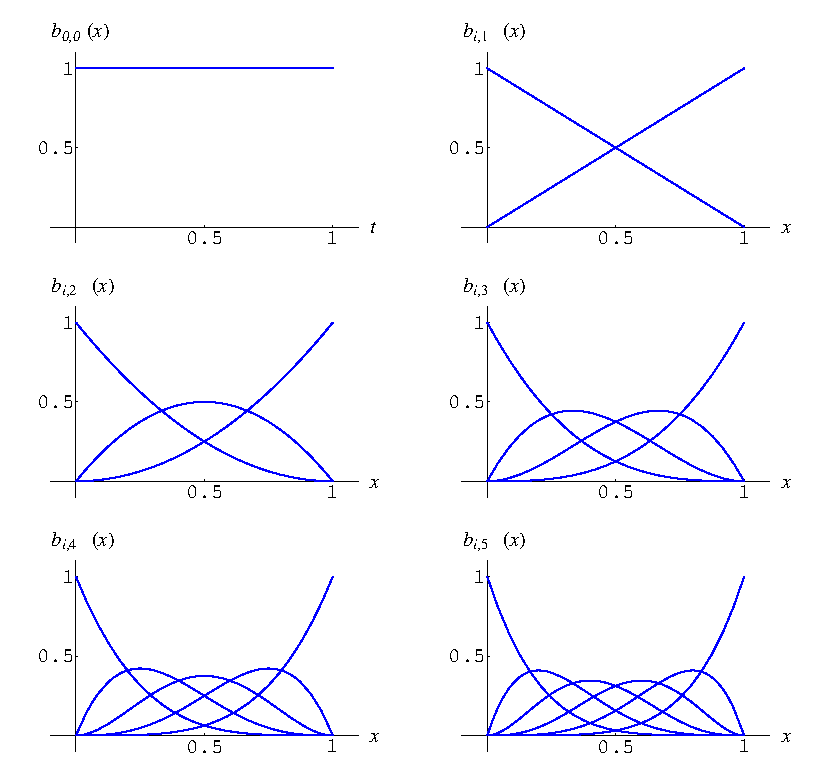
\includegraphics[width=\textwidth]{fig/BernsteinPol}
\caption{The Bernstein polynomials up to order $n=5$.\label{fig:BerPol}}
\end{center}
\end{figure}
\subsection{B\'ezier splines}
B\'ezier splines are curves defined on an interval for a parameter $t\in [0,1]$.
They are controlled by points that contribute to the curve parametrized by $t$
with a fixed weighting function in $t$. Two point, e.g., produce a straight
line, a so called linear B'ezier curve, to read
\[     \mathbf{B}(t)=\mathbf{P}_0 + t(\mathbf{P}_1-\mathbf{P}_0)=(1-t)\mathbf{P}_0 + t\mathbf{P}_1 \mbox{ , } t \in [0,1] \]
A cubic B\'ezier spline reads
\[     \mathbf{B}(t)=(1-t)^3\mathbf{P}_0+3(1-t)^2t\mathbf{P}_1+3(1-t)t^2\mathbf{P}_2+t^3\mathbf{P}_3 \mbox{ , } t \in [0,1]\]
A B\'ezier curve of degree $n$ reads
\[ \mathbf{B}(t)=\sum_{i=0}^n \binom{n}{i}(1-t)^{n-i}t^i\mathbf{P}_i =(1-t)^n\mathbf{P}_0+\binom{n}{1}(1-t)^{n-1}t\mathbf{P}_1+\cdots+t^n\mathbf{P}_n \mbox{ , } t \in [0,1]\]
Observe that in order to adjust the path the curve must follow you have to move
the control points. The extension to surfaces is straight forward
\[ x(s,t)=\sum_{i=0}^n \sum_{j=0}^m B_i^n(s) \; B_j^m(t) \; \mathbf{k}_{i,j}\]
where the $B_i^n(\nu)$ are the Bernstein polynomials and the $\mathbf{k}_{i,j}$ are the $(n+1)(m+1)$ control points.
\subsection{Legendre Polynomials}
Legendre polynomials are defined as
\begin{equation}
	    P_n(x) = \frac{1}{2^n n!}\frac{d^n}{dx^n } \left[ (x^2 -1)^n \right]
	\label{eq:legendre}
\end{equation}
They derive from the solution of the following differential equation
\[\frac{d}{dx} \left[ (1-x^2)\frac{d}{dx} P_n(x) \right] + n(n+1)P_n(x) = 0\]
Legendre polynomials are orthogonal on the interval $[-1,1]$, i.e.
\[     \int_{-1}^{1} P_m(x) P_n(x)\,dx = \frac{2}{2n + 1} \delta_{mn} \]
holds.

The first six Legendre polynomials read
\begin{eqnarray*}
 	P_0(x)=1\\
	P_1(x)=x\\
	P_2(x)=\frac{1}{2} (3x^2-1) \\
	P_3(x)=\frac{1}{2} (5x^3-3x) \\
	P_4(x)=\frac{1}{8} (35x^4-30x^2+3)\\
	P_5(x)=\frac{1}{8} (63x^5-70x^3+15x)
\end{eqnarray*}
\section{Numerical integration}
Numerical integration must be used if:
\begin{itemize}
	\item The integral cannot be evaluated analytically
	\item The integrand is not given in analytical form but rather
		numerically with a certain number of dicrete values
\end{itemize}
		
\subsection{Trapezoid quadrature}
This method consists in replacing the given function $f(x)$ by a set of lines connecting the sample points and then to sum all the trapezoid areas to approximate the integral, to give
\begin{eqnarray*}
	\int_{x_{i-1}}^{x_i}f(x)dx&\approx &\frac{f_{i-1}+f_i}{2}\Delta x_i\\
	\Delta x_i&=&x_i-x_{i-1}
\end{eqnarray*}
$[a,b]$ be the interval of integration. With $x_0=a,\; x_1,\dots,\; x_n=b$ we have
\begin{equation}
	\int_{a}^{b}f(x)dx\approx \sum_{i=1}^n\frac{f_{i-1}+f_i}{2}\Delta x_i
	\label{eq:trapez}
\end{equation}
Suppose that we have regularly spaced sample points
\[ \Delta x_i=\Delta x=\frac{b-a}{n} \]
Then (\ref{eq:trapez}) reads
\[\int_a^bf(x)dx\approx\frac{\Delta x}{2}\left[ f_0+f_n+2\sum_{i=1}^{n-1}f_i\right]\]
This does not allow to tell about the integration error. For this we have to
expand the function into a Taylor series to first order and one replaces the
function by a secant neglecting second order terms in $\Delta x$. One can show
that
\begin{equation}
	\int_a^bf(x)dx=\frac{\Delta x}{2}\left[ f(a)+f(b)+2\sum_{i=1}^{n-1}f(x_i)\right]
	-\frac{(\Delta x)^2}{12}(b-a)f''(\bar{x})-{\cal O}(\Delta x^4)
	\label{eq:order4}
\end{equation}
where $\bar{x}\in[a,b]$. In most cases one obtains a better approximation
of the integral, if one writes for the second derivative
\[ f''(\bar{x})=\frac{f'(a)-f'(b)}{b-a} \]
to give
\begin{equation}
        \int_a^bf(x)dx=\frac{\Delta x}{2}\left[ f(a)+f(b)+2\sum_{i=1}^{n-1}f(x_i)\right]
        -\frac{(\Delta x)^2}{12}\left[ f'(b)-f'(a)\right]
        \label{eq:order4apr}
\end{equation}
(\ref{eq:order4apr}) is the trapezoid form with corrections at the
endpoints. With this the methods becomes a 4th order method
%\subsection{Example}
\subsection{Integration using Interpolation}
We consider an interpolating polynomial with the support points given as
$a\le x_0\le x1\le\dots\le x_n\le b$
and, e.g. Lagrange polynomials as interpolation functions
\[ p_n[x]=\sum_{k=0}^nf[x_k]L_k[x]\]
Integration of the polynomial yields
\[ Q-n=\int_a^bp_n[x]dx=\sum_{k=0}^nf[x_k]\int_a^bL_k[x]dx=(b-a)\sum_{k=0}^nw_kf[x_k] \]
where the weights are defined as
\[ w_k=\frac{1}{(b-a)}\int_a^bL_k[x]dx\]

\begin{note}{}
If $f(x)$ is a polynomial of degree $<n+1$, then $p_n(x)$ is exact, and thus
also $Q_n$ is exact.
\end{note}
\subsection{Simpson's rule}
This method consists in replacing the function $f(x)$ between $x_{i-1}$ and
$x_{i+1}$ by a parabola passing through $f_{i-1}$, $f_i$, and $f_{i+1}$. One
can show the Simpson rule by a Taylor expansion of the integral. To this end we
write
\[ I(x)=\int_a^x f(x')dx'\]
It is
\[ \frac{dI(x)}{dx}=f(x)\]
The integral over the interval between $x_{i-1}$ and $x_{i+1}$ can now be written as
\[ A_i =I(x_{i+1})-I(x_{i-1})\]
If we do this for all intervals and sum, we get
\[\int_a^bf(x)dx=\frac{\Delta x}{3} \left[
f(a)+f(b)+4 \sum_{\substack{i=1\\ odd}}^{n-1} 
A_i+2 \sum_{\substack{i=2 \\ even}}^{n-2}A_i\right]+{\cal O}(\Delta x^4)\]

\subsection{Gau{\ss} quadrature}
This very precise method uses non uniformly distributed discretization points,
which are chosen to the best convenience. This method can be applied when the
integrand $f(x)$ is known analytically or if its values are known exactly where
the support points for the method have to be located. It might not be applied,
whenever a discrete representation of $f(x)$ does not fulfil these
requirements.

As we have already shown in the previous section, one can use an interpolation
of the function $f(x)$ in terms of polynomials, in order to write the integral
of this function as a weighted sum over its function values at specific points
\[ \int_{a}^{b}f(x)dx=C\sum_{k=1}^nw_kf(x_k)\]
where $C$ is proportional to $b-a$. The weighting factors $w_k$ depend on the
specific function that approximates $f(x)$. These are straight line segments is
the case of trapezoid quadrature, or parabolas in case of the method by
Simpson.

In the method by Gauss $f(x)$ is approximated by a basis of orthogonal
polynomials. The $x_i$ are the roots of these polynomials and thus are
irregularly spaced. One can use any kind of polynomials, e.g. Jacobi,
Tchebychev, Laguerre, Hermite\dots, but the most often used are those of
Legendre. These are defined in the interval $[-1,1]$. To this end we have to
change the variable, which is $x\in[a,b]$, by means of a linear transformation
to become $\xi\in[-1,1]$. This transformation reads
\[x=\frac{b+a}{2}+\frac{b-a}{2}\xi \]

Thus we have
\[\int_a^bf(x)dx=\frac{b-a}{2}\sum_{k=1}^{n}w_kf(x_k)\]
where the $w_k$ and the $\xi_k$ are given in the following table
\begin{center}
\begin{tabular}{|c|c|c|}
\hline
n&$\pm\xi_k$&$w_k$\\\hline
2&0.5773502692&1.0000000000\\\hline
3&0.0000000000&0.8888888889\\
 &0.7745966692&0.5555555556\\\hline
4&0.8611363116&0.3478548451\\
 &0.3399810436&0.6521451549\\\hline
5&0.0000000000&0.5688888889\\
 &0.5384693101&0.4786286705\\
 &0.9061798459&0.1713244924\\\hline
\end{tabular}
\end{center}

We shall not derive this method but rather give some arguments why it works.
One can show that the method is exact for polynomials of order $2n-1$. To see
this take such a polynomial $p(x)$ and represent it the following way
\[ p(x)=q(x)P_n(x) +r(x)\]
where $P_n(x)$ is a Legendre polynomial of order $n$, $q(x)$ is a polynomial of
order $n-1$ as well as is the rest $r(x)$. 
We thus have
\[ \int_{-1}^1p(x)dx=\int_{-1}^1q(x) P_n(x) dx+\int_{-1}^1r(x)dx=\int_{-1}^1r(x)dx\]
Now choose as support points the roots of $P_n(x)$ and we have the same result
from the quadrature formula
\[ \sum_{k=1}^nw_kp(x_k)=\sum_{k=1}^nw_kq(x_k)P_n(x_k)
+\sum_{k=1}^nw_kr(x_k)=\sum_{k=1}^nw_kr(x_k)\]
Now, the interpolation quadrature
formula of $x_k$ has accuracy of $2n-1$, and delivers the exact value for the
polynomial $L_k(x)^2$. Therefore we have
\[ w_k=\int_{-1}^1L_k(x)^2dx=\int_{-1}^1\prod_{\substack{j=1\\ j\neq
k}}\left(\frac{x-x_j}{x_k-x_j}\right)^2=\sum_{\mu=1}^nw_\mu L_k(x_\mu)^2\]

This gives a recipe how the $x_k$ and the $w_k$ must be chosen to get the
desired accuracy.
\subsection{Integrals of functions with multiple variables}
The multidimensional integral
\[ \int_{a_n}^{b_n}\ldots\int_{a_2}^{b_2}
\int_{a_1}^{b_1}f(x_1,x_2,\ldots,x_n)dx_1dx_2\cdots dx_n\]
must be progressively replaced by a quadrature formula
\[ \sum_{i_1=0}^{k_1}w_{i_1}\int_{a_2}^{b_2}\ldots
\int_{a_n}^{b_n}f(x_{i_1},x_2,\ldots,x_n)dx_1dx_2\cdots dx_n\]
to give
\[ \sum_{i_1=0}^{k_1}\sum_{i_2=0}^{k_2}\ldots
\sum_{i_n=0}^{k_n} w_{i_1} w_{i_2}\ldots w_{i_n}
f(x_{i_1},x_ {i_2},\ldots,x_ {i_n})\]
For high dimensional spaces of the function argument this can very easily end
in a tremendous computational load. In this case other methods must be provided
which are not subject of the discussion here.

%
\begin{appendices}
\noappendicestocpagenum
\renewcommand\appendixtocname{Anhang}
\renewcommand\appendixpagename{Anhang}
\chapter{Der Residuensatz}\label{sec:Residuensatz}
Die Funktion $f(z)$ der komplexen Zahl $z=x+iy$ schreiben wir als Summe des
Real- und Imaginärteils $f(z)=u(x,y)+iv(x,y)$.
\begin{example}{Komplexe Funktionen}
  Verifiziere:
  \[ z^2=\underbrace{(x^2-y^2)}_{u(x,y)}+\underbrace{i2xy}_{v(x,y)}\]
  \[\sin(z)=\underbrace{\sin(x)\cosh(y)}_{u(x,y)}+i\cdot\underbrace{\cos(x)\sinh(y)}_{v(x,y)}\]
\end{example}

\begin{wrapfigure}[12]{l}{0.45\textwidth}
 \begin{center}
  \begin{tikzpicture}[thick]
   \draw[->] (-2.5,0) -- (2.5,0) node[right] {x};
   \draw[->] (0,-.5) -- (0,2.5) node[above] {y};
   \draw[->] (-2,0.02) -- (2,0.02);
   \draw[->] (2,0) arc (0:180:2);
   %
   \draw (-2.,0) -- (-2.,-.1) node[below] {$-\rho$};
   \draw (2.,0) -- (2.,-.1) node[below] {$\rho$};
   \node at (1.6,1.6) {C};
   %
  \end{tikzpicture}
  \caption{Integrationsweg in der komplexen Ebene.\label{fig:Halbkreis}}
 \end{center}
\end{wrapfigure}
Ein Integral im Reellen, also z.B. $I=\int f(x)dx$, wird im komplexen zu einem
Linienintegral im zweidimensionalen Raum der durch $x,y$ aufgespannt wird.
Deshalb müssen wir zusätzlich noch den Integrationsweg angeben. In
Parameterform würde das bedeuten, wir müssen die Funktionen $x(s)$ und $y(s)$
angeben für ein Intervall von $s$.

Wir sind speziell an geschlossenen Intagrationswegen in der komplexen Ebene interessiert:
$I=\oint f(z)dz$, wie z.B. dem geschlossenen Halbkreis in Abbildung
\ref{fig:Halbkreis}. Auf diesem Integrationsweg wollen wir das Integral der Funktion
\[f(z)=\frac{e^{ikz}}{z^2+\Gamma^2}\]
angeben. Mit $z=\rho e^{i\varphi}$ ist $dz=e^{i\varphi}d\rho+i\rho
e^{i\varphi}d\varphi$.  Damit setzt sich das Integral aus zwei Anteilen
zusammen, das Integral über die reelle Achse von $-\rho$ bis $\rho$ und das
über den Halbkreis
\[\oint f(z)dz=\int\limits_{\substack{-\rho\\ (dy=0)}}^{\rho}\frac{e^{ikx}}{x^2+\Gamma^2}dx+
  \int\limits_{\substack{0\\(d\rho=0)}}^{\pi}\frac{e^{i\varphi}
  e^{i\rho k\cos(\varphi)-\rho k\sin(\varphi)}}{\rho^2e^{i2\varphi}+\Gamma^2}d\varphi
\]
Dabei wird als Parameter $s$ im ersten Summanden $x$ benutzt, denn auf dem
Teilstück des Wegs ist $y=0$. Im zweiten Summanden hingegen ist $\rho=const.$
und damit $\varphi$ als Parameter zu nehmen.

Im Limes $\rho\rightarrow\infty$ verschwindet der zweite Summand in obiger
Gleichung und wir erhalten
\[\lim_{\rho\rightarrow\infty}\oint f(z)dz=
  \int\limits_{\substack{-\rho\\ (dy=0)}}^{\rho}\frac{e^{ikx}}{x^2+\Gamma^2}dx=
\int\limits_{\substack{-\rho\\ (dy=0)}}^{\rho}\frac{\cos(kx)}{x^2+\Gamma^2}dx=\frac{\pi}{\Gamma}e^{-k\Gamma}
\]
Für die Berechnung von Integralen dieser Art benutzen wir den {\it
Residuensatz}. Dazu müssen wir noch den Begriff der Pole einer Funktion $f(z)$
klären. Die Funktion $f(z)$ hat an der Stelle $z=z_r$ einen {\it Pol 1. Ordnung}, wenn gilt
\[\lim_{z\rightarrow z_r}(z-z_r)f(z)\ne 0,\]
oder einen {\it Pol m-ter Ordnung}, wenn gilt
\[\lim_{z\rightarrow z_r}(z-z_r)^mf(z)\ne 0.\]
Die den Polen m-ter Ordnung zugeordneten Residuen sind definiert als
\begin{equation}
  \text{Res }\left.f(z)\right|_{z=z_r}=\lim_{z\rightarrow z_r}\frac{1}{(m-1)!}
    \frac{d^{m-1}}{dz^{m-1}}\left[(z-z_{r})^{m}f(z)\right]
  \label{eq:Residuum}
\end{equation}

Nun sind wir in der Lage den Residuensatz zu formulieren.
\begin{satz}{Residuensatz}
  Der Wert eines geschlossenen Integrals in der Ebene ist gleich dem $2\pi
  i$-fachen der Summe der umschlossenen Residuen.
  \begin{equation}
    \oint f(z)dz=2\pi i\sum\limits_{\substack{r=1\\ (z_r\text{ innerhalb }C)}}\text{Res }\left.f(z)\right|_{z=z_r} 
      \label{eq:Residuensatz}
  \end{equation}
\end{satz}


\chapter{Interpolation und Integration}
%{\bf Learning goals:}
%\begin{itemize}
%\item Represent discrete data as functions to obtain function values apart from
%	the support points
%\item Increase presision at lower cost, i.e. few parameters together with
%	interpolating functions cover the whole space
%\item Fast numerical integration by using interpolated representations of
%	functions with a limited number of interpolating functions.
%\end{itemize}\newpage
\section{Diskrete Daten und Interpolationsfunktionen}
\subsection{Das Newton Polynom}\label{subsec:newton}
Gegeben eine funktion $f(x)$, die an einer endlichen Zahl von Punkten $x_i$ bekannt sei.
Wir haben $f(x_i)=y_i$.  Es seien $n+1$ Paare $P_i=(x_i,y_i)$ von Werten gegeben, die Stützstellen
Wir wollen uns eine pllynomiale Funktion n-ter Ordnung beschaffen, geschrieben als
\[p_n(x)=a_0+a_1 x+\dots +a_n x^n\]
für die
\[p_n(x_i)=a_0+a_1 x_i+\dots +a_n x_i^n=y_i\]
gilt. Das Newton'sche polynomoiale Approximationsschema ist das meistbenutzte,
da es unter anderem auch für irregulär verteilte Stützstellen funktioniert.
Darüberhinaus muss der Polynomgrad nicht a priori festgelegt werden.
\subsubsection{Dividierte Differenzen}
Dividierte Differenzen sind durch eine rekursive Division definiert. Sie sind sein nützliches Werkzeug, um die Koeffizienten von Interpolationspolynomen zu berechnen.
Für jede geordnete Folge von Stützstellen 
$x_k$, mit $k=0,1,\dots,n$ ist der Algorithmus zur Berechnung der dividierten Differenzen für eine Untermenge der Stützstellen gegeben als
\begin{eqnarray}
	\label{eq:divdiffs}
   D[x_i] f&=& f(x_i)=f_i, \qquad \nu \in \{ 0,\ldots,n\}\\
   D[x_i,x_j] f&=& \frac{f_j-f_i}{x_j-x_i}\nonumber\\
   D[x_i,x_j,x_k] f&=& \frac{D[x_j,x_k]f-D[x_i,x_j]f}{x_k-x_i}\nonumber\\
   D[x_i,x_j,\ldots,x_l,x_m] f&=& \frac{D[x_j,\dots,x_m]f-D[x_i,\dots,x_l]f}{x_m-x_i}\nonumber
\end{eqnarray} 
Manchmal ist ed bequemer die folgende Matrixnotation zu benutzen
\begin{equation} 
	D_{i,j}=D[x_i,x_{i+1},\dots,x_{i+j}]f
	\label{eq:invdivdiffs}
\end{equation}
\subsubsection{Berechnung der Newton'schen Form}
Wir wollen $f(x)\approx p_n(x)$ finden, wobei $p_n(x)$ ein Newton'sches Polynom
ist, gegeben durch die Punkte $(x_0,f_0),\dots,(x_n,f_n)$, das folgendermaßen
definiert sei
\begin{equation}
	p_n(x)=f_0+(x-x_0)D[x_0,x_1]f+\dots +(x-x_0)\cdots (x-x_{n-1})D[x_0,\dots,x_n]f
	\label{eq:newtonpoly}
\end{equation}
oder mit der oben erwähnten Matrixform der dividierten Differenzen
\[
p_n(x)=D_{0,0}+D_{0,1}(x-x_0)+\dots +D_{0,n}(x-x_0)\cdot(x-x_{n-1})=D_{0,0}+\sum_{k=1}^nD_{0,k}\prod_{j=0}^{k-1}(x-x_j)
\]
Der größte Vorteil der hier präsentierten Methode ist, dass die dividierten Differenzen 
$D_{i,k}$ eng mit der k-ten Ableitung am Punkt $i$ verbunden sind.  Es ist
hiermit möglich zu entscheiden, ob eine Funktion, die durch ein Anzahl von
Stützstellen gegeben ist,  durch ein Polynom k-terOrdnung approximierbar ist.  Anders
gesagt, wenn alle Koeffizienten der  Matrixform der dividierten Differenzen in
der k-ten Spalte von derselben Größenordnung sind, d.h.  $D_{0,k}\approx
D_{0,1}\approx D_{0,2}\approx\dots$.
\subsection{Lagrangeinterpolation}
Lagrangepolynome sind so konstruiert, dass Sie durch alle Stützstellenpunkte, wie in \ref{subsec:newton}, gehen.
\[
L_i(x)=\prod_{j=0,j\neq i}^n\frac{(x-x_j)}{x_i-x_j}=\frac{(x-x_0)\ldots(x-x_{i-1})(x-x_{i+1})\ldots(x-x_n)}{(x_i-x_0)\ldots(x_i-x_{i-1})(x_i-x_{i+1})\ldots(x_i-x_n)}
\]
Wie man leicht sieht ist
\[
L_i(x)=\left\{
\begin{array}{rcl}
1&\mbox{ für }&x=x_i\\ 
0&\mbox{ für }&x=x_{j\ne i}
\end{array}\right.
\]
oder in Anderen Worten $L^n_j(x_i)=\delta_{ij}$. Das Polynom, das durch die 
$n+1$ Interpolationspunkte geht, schreibt man
\[ p_n(x)=\sum_{i=0}^n y_i\ L_i(x) \]
\subsubsection{Alternative Form  der Langrangeinterpolationsformeln}
Dieses Polynom stimmt mit der Funktion $f(x)$ an den Abszissen der Interpolationspunkte $x_i$ exakt überein. Neben $x_i$ tritt i. A. ein Fehler auf, der aber bestimmbar ist. Wir schreiben das Polynom um
\[ p_n(x)=\sum_{i=0}^n y_i\ \prod_{j=0,j\neq i}^n\frac{x-x_j}{x_i-x_j}=
\sum_{i=0}^n y_i 
\underbrace{
\frac{1}{x-x_i} \prod_{j=0,j\neq i}^n\frac{1}{x_i-x_j} 
}_{\mu_i}\ 
\underbrace{\prod_{k=0}^n (x-x_k)}_{l(x)}
\]
Es gibt eine alternative Schreibweise für das Polynom
\begin{equation}\label{eq:1stbarycentric}
	p_n(x) = l(x)\sum_{i=0}^n \mu_iy_i,
\end{equation}
gemeinhin als baryzentrische Interpolationsformel bezeichnet. Wenn wir verlangen, dass $p_n(x)=1$ sehen wir, dass $y_i=1$ und deshalb haben wir
\[ 1 = l(x)\sum_{i=0}^n \mu_i \]
Teilen wir (\ref{eq:1stbarycentric}) durch letzteres, dann erhalten wir die zweite baryzentrische Form
\begin{equation}
	p^n(x)=\frac{\sum_{i=0}^n \mu_iy_i}{\sum_{i=0}^n \mu_i}
	\label{eq:2ndbarycentric}
\end{equation}
%The $n+1$ Lagrange polynomials of order n add up to unity everywhere in the interval.
\subsubsection{Interpolationspunkte gleichen Abstands}
Für Interpolationspunkte gleichen Abstands $x_i-x_{i-1}=h$ erhalten wir
\begin{eqnarray*}
\lambda_i =\prod_{j=0,j\neq i}^n\frac{1}{x_i-x_j} 
&=&\frac{1}{(-1)^{n-i}h^n(i(i-1)(i-2)\ldots1)(1\ 2\ \ldots\ (n-1))}\\[1ex]
&=&\frac{(-1)^{n-i}}{h^n n!}
\left(\begin{array}{c}n\\ i\end{array}\right)
\end{eqnarray*}
In diesem Fall können wir  
\[
\mu_i=\frac{1}{x-x_i} \prod_{j=0,j\neq i}^n\frac{1}{x_i-x_j}=
\frac{1}{x-x_i} \lambda_i
\]
schreiben. Wenn wir beachten, dass in (\ref{eq:2ndbarycentric}) alle Faktoren
im Zaähler und Nenner, über die nicht summiert wird, sich wegheben, dann
erhalten wir die einfache Form
\[ 
  \lambda_i^* = (-1)^i\left(\begin{array}{c}n\\ i\end{array},\right)
\]
die $\lambda_i$ für unregelmäßige Abstände der Interpolationspunkte ersetzt..
\subsubsection{Application of Lagrange polynomials}
For a given number of sample points let us calculate the derivative of the
Lagrange polynomial, to read
\[ 
\frac{d^n p_n(x)}{dx^n}=\sum_{i=0}^ny_i\lambda_in!\approx f^{(n)}(x)
\]
The latter is an approximation for the derivative of the interpolated function.
We consider an equidistant set of sample points $x_i=x_{i-1}+h,\ \ \ x_i=x_0+i
h$ and an interpolation of second order, which reads
\[
~p_2(x)=\frac{1}{2h^2}
\left( y_0(x-x_1)(x-x_2)
     -2y_1(x-x_0)(x-x_2)
      +y_2(x-x_0)(x-x_1)\right)
\]
Its derivative reads
\[
p_2'(x)=\frac{1}{2h^2}
\left( y_0(2x-x_1-x_2)
     -2y_1(2x-x_0-x_2)
      +y_2(2x-x_0-x_1) \right)
\]
Thus we have the approximations for the derivatives at the sample points given
as
\begin{equation}\label{eq:leftderiv} 
f'(x_0)\approx\frac{1}{2h}\left({-3y_0+4y_1-y_2}\right)
\end{equation}
\begin{equation}\label{eq:centerderiv}
f'(x_1)\approx\frac{1}{2h}\left({-y_0+y_2}\right)
\end{equation}
\begin{equation}\label{eq:rightderiv}
f'(x_2)\approx\frac{1}{2h}\left({-y_0+4y_1-2y_2}\right)
\end{equation}
\subsubsection{Alternate formulation}
Let us use the alternate formulation for equidistant sample points. For
the $\lambda_i$ and $\mu_i$ we have 
\begin{eqnarray*}
\lambda_0&=&\frac{1}{(x_1-x_0)(x_2-x_0)}=\frac{1}{2h^2}\\
\lambda_1&=&\frac{1}{(x_0-x_1)(x_2-x_1)}=-\frac{1}{h^2}\\
\lambda_2&=&\frac{1}{(x_0-x_2)(x_1-x_2)}=\frac{1}{2h^2}
\end{eqnarray*}
and
\begin{eqnarray*}
\mu_0&=&\lambda_0\frac{1}{(x-x_0)}=\frac{1}{2h^2 (x-x_0)}\\
\mu_1&=&\lambda_1\frac{1}{(x-x_1)}=-\frac{1}{h^2 (x-x_1)}\\
\mu_2&=&\lambda_2\frac{1}{(x-x_2)}=\frac{1}{2h^2 (x-x_2)}
\end{eqnarray*}
While the reduced quantities read
\begin{eqnarray*}
\lambda^*_0&=&(-1)^0\left(\begin{array}{c}2 \\ 0\end{array}\right)=1\\
\lambda^*_0&=&(-1)^1\left(\begin{array}{c}2 \\ 1\end{array}\right)=-2\\
\lambda^*_0&=&(-1)^2\left(\begin{array}{c}2 \\ 2\end{array}\right)=1
\end{eqnarray*}
and
\begin{eqnarray*}
\mu_0^*&=&\lambda_0^*\frac{1}{(x-x_0)}=\frac{1}{(x-x_0)}\\
\mu_1^*&=&\lambda_1^*\frac{1}{(x-x_1)}=-\frac{2}{(x-x_1)}\\
\mu_2^*&=&\lambda_2^*\frac{1}{(x-x_2)}=\frac{1}{(x-x_2)}
\end{eqnarray*}
And finally we obtain
\[
p_2(x)=\frac{\displaystyle\sum_{i=0}^2 \mu_iy_i}{\displaystyle\sum_{i=0}^n \mu_i}
=\frac{(x-x_1) (x-x_2) y_0 -2(x-x_0) (x-x_2) y_1+ (x-x_0) (x-x_1) y_2}{2h^2}
\]
\subsection{Interpolation by continued fraction}
Some functions $f(x)$ cannot be approximated well by polynoms, since they
contain horizontal or vertical aymptotes. In these cases it is convenient to
approximate $f(x)$ by a limited continued fraction.

It is possible to expand $f(x)$ in a continuous fraction provided one can write
\begin{equation}
	f(x)=y_0+\cfrac{x-x_0}{y_1+\cfrac{x-x_1}{y_2+\cfrac{x-x_2}{y_3+\cdots}}}
	\label{eq:contfrac}
\end{equation}
The expansion given in (\ref{eq:contfrac}) is limited to a finite order for
practical reasons, i.e.\ it is a truncated continuous fraction. $f(x)$ is known
through its values $f_j=f(x_j)$ at the support points $x_j$, with
$j=0,1,\dots,n$. The $y_k$ may be expressed by means of the inverse divided
differences $d_{ij}$, which are given by
\begin{eqnarray}
	d_{i,0}f&=&f_i\mbox{, for }i=0,\dots,n\nonumber\\
	d_{i,1}f&=&\frac{x_{i+1}-x_i}{f_{i+1}-f_i}\mbox{, for }i=0,\dots,n-1\label{eq:invdivdif}\\
	d_{i,j}f&=&\frac{x_{i+1}-x_i}{f_{i+1}-f_i}+d_{i+1,j-2}f\mbox{, for }j=2,\dots,n\mbox{ and }i=0,\dots,n-j\nonumber
\end{eqnarray}
Thus we have 
\[
y_0=f_0,\ y_1=d_{0,1}f,\ y_k=d_{0,k}f-d_{0,k-2}\mbox{ with }2\le k\le n
\]
Having calculated the values $y_0,y_1,\dots,y_n$ we obtain a continuos fraction
truncated at the term $(x-x_{n-1}/y_n$, that allows to calculate an
interpolated value of $f$ at $x$ through the recursive relation
\begin{eqnarray*}
	F_n(x)&=&y_n\\
	F_k(x)&=&y_k+\frac{x-x_k}{F_{k+1}(x)}\mbox{ with }k=n-1\mbox{ to }0\\
	f(x)&=&F_0(x)
\end{eqnarray*}

\begin{example}{Interpolation}
	\label{ex:contfrac}
Interpolate at $x=3.5$ the function $f(x)$ given through
\begin{center}
\begin{tabular}{c|rrrrr}
	$x_i$&-2&0&2&3&4\\\hline
	$f_i$&2&0&-10&-33&-124
\end{tabular}
\end{center}
Applying the above algorithm (verify!) we find the expansion
\begin{equation}
f(x)=-124+\cfrac{x-4}{\frac{-1}{91}+\cfrac{x-3}{\frac{5187}{34}+\cfrac{x-2}{\frac{680}{3913}+\cfrac{x}{\frac{-903}{34}}}}}
	\label{eq:excontfrac}
\end{equation}
\end{example}

\subsection{Spline interpolation}
A spline is a thin wood or metal strip used in building construction. The most
useful spline functions follow the same constraints as bent metal or wooden
strips, they tend to minimize curvature. Our starting point is again the set of
collocation points $(x_i,y_i)$. We are looking for a function $sp(x_i)=y_i$
that connects all the collocation points and that respects certain constraints.
Linear connections between the collocation points are simple traverses of
linear functions that connect the collocation points. The only constraints that
seem to make sense in this case are that the endpoints of the lines go through
the collocation points. If we allow higher order polynomial functions to connect
the sample points, we might ask for more complicated constraints to be
respected. A spline ist a set of polynomes of 3rd degree that connect the
collocation points. Our task will be to find the coefficients of the single
polynomes, given the constaints.

Assume that we want to minimize the overal bending energy of the spline, given by
\begin{equation}
	S=\int_{x_0}^{x_n}\left(\frac{d^2 s(x)}{dx^2}\right)^2dx
	\label{eq:bendingE}
\end{equation}
This is equivalent to the requirement that the variation $\delta S$ of $S$ vanishes, i.e.
\begin{equation}
	\delta S=\int_{x_0}^{x_n} s''(x) \delta s''dx=0
	\label{eq:Evar}
\end{equation}
We divide the integral in intervals given by the positions of the collocation points
\begin{equation}
	\delta S=\sum_{i=0}^{n-1}\int_{x_i}^{x_{i+1}} s''(x) \delta s''dx=0
	\label{eq:Evarint}
\end{equation}
At the supports the variation $\delta s''(x_j)=0$.

In order to solve for the coefficients of the set of polynomes, let us
transform (\ref{eq:Evarint}) with the help of partial integration.

\begin{note}{} 
	Partial integration means $\int f\ dg = f\cdot g - \int g\ df$.
\end{note}

We have
\[
\int_{x_{i-1}}^{x_i}s''(x)\delta s'' (x) dx=\int_{x_{i-1}}^{x_i}s''(x)d(\delta s' (x))= \left. {s''(x)\delta s'(x)}\right|_{x_{i-1}}^{x_i}-\int_{x_{i-1}}^{x_i}\delta s' (x)d(s''(x))
\]
\begin{eqnarray*}
\int_{x_{i-1}}^{x_i}\delta s' (x)d(s''(x))=\int_{x_{i-1}}^{x_i}s'''(x)\delta s' (x)dx&=&
\int_{x_{i-1}}^{x_i}s'''(x)d(\delta s(x))\\[1ex]
&=&\left. {s'''(x)\delta s(x)}\right|_{x_{i-1}}^{x_i}-\int_{x_{i-1}}^{x_i} \delta s(x) d(s'''(x))
\end{eqnarray*}
\[
\int_{x_{i-1}}^{x_i} \delta s(x) d(s'''(x))=\int_{x_{i-1}}^{x_i} s''''(x)\delta s(x) dx
\]
It is
\[
d(s'''(x))= \frac{d(s'''(x))}{dx}dx= s''''(x) dx
\]
The variation of the integral (\ref{eq:Evarint})
finally reads
\begin{eqnarray*}
\sum_{i=1}^n\int_{x_{i-1}}^{x_i}s''(x)\delta s'' (x)dx
&=&\sum_{i=1}^n\left(\left. s''(x)\delta s'(x)\right|_{x_{i-1}}^{x_i}-\left.
s'''(x)\delta s(x)\right|_{x_{i-1}}^{x_i}\right. \\[1ex]
&&\left. -\int_{x_{i-1}}^{x_i} s''''(x)\delta s(x)dx\right)
\end{eqnarray*}
Remember that this must hold for arbitrary variations $\delta$ - besides at $x_0$ and $x_n$ where $\delta s=0$ holds - and thus their coefficients must vanish. 
\begin{eqnarray*}
s''''(x)&=&0 \text{ for } x\neq x_i
\\
s''(x_0)&=&s''(x_n)=0
\\
s''(x_i)^+&=&s''(x_i)^-,\ \ \ i=1,2,\ldots,n-1
\end{eqnarray*}

Consider the interval $[x_i,x_{i+1}]$ where $h_i=x_{i+1}-x_i$. The coefficients
of the cubic polynomial
\[ a_i(x)=a_i(x-x_i)^3+b_i(x-x_i)^2+c_i(x-x_i)+d_i \]
are to be determined. Compute the value of the polynomial and its first and
second derivatives at each of the two endpoints to give
\begin{eqnarray}
	  a_i&=&\frac{1}{6h_i}(y^{\prime\prime}_{i+1}
	        -y^{\prime\prime}_{i})\label{eq:splinecoefai} \\
	  b_i&=&\frac{1}{2} y^{\prime\prime}_{i}\label{eq:splinecoefbi}\\
	  c_i&=&\frac{1}{h_i}(y_{i+1}-y_i)-\frac{1}{6}h_i (y^{\prime\prime}_{i+1}
	        -y^{\prime\prime}_{i})\label{eq:splinecoefci}\\
	  d_i&=&y_i\label{eq:splinecoefdi}
  \end{eqnarray}
Thus in all intervals we have related the coefficients of the repective polynom
to the second derivative at the endpoints of the interval
(\ref{eq:splinecoefai}-\ref{eq:splinecoefdi}). The final task is to find an equation system to solve
for the $y_i''$.

\begin{example}{Spline interpolation on 5 intervals}
	\begin{eqnarray*}
		\lefteqn{\left(
		\begin{array}{cccc}
			2(h_0+h_1)&h_1&0&0\\
			h_1&2(h_1+h_2)&h_2&0\\
			0&h_2&2(h_2+h_3)&h_3\\
			0&0&h_3&2(h_3+h_4)
		\end{array}
		\right)\cdot
		\left(
		\begin{array}{c}
			y^{\prime\prime}_1\\
			y^{\prime\prime}_2\\
			y^{\prime\prime}_3\\
			y^{\prime\prime}_4
		\end{array}
		\right)
		=}\hspace{7cm}\\
		&&\left(
		\begin{array}{c}
			\frac{6}{h_0}(y_1-y_0)+\frac{6}{h_1}(y_2-y_1)+h_0y_0^{\prime\prime}\\
			\frac{6}{h_1}(y_2-y_1)+\frac{6}{h_2}(y_3-y_2)\\
			\frac{6}{h_2}(y_3-y_2)+\frac{6}{h_3}(y_4-y_3)\\
			\frac{6}{h_3}(y_4-y_3)+\frac{6}{h_4}(y_5-y_4)+h_4y_5^{\prime\prime}
		\end{array}
		\right)
	\end{eqnarray*}
\end{example}

\subsection{Bernstein Polynomials}
Any interval $[a,b]$ can be mapped to the unit interval $[0,1]$ by the transformation
\[
\lambda=(t-a)/(b-a)
\]
The Bernstein basis polynomials are defined on the unit interval as
\begin{equation}
	 b_{\nu,n}(x) = \binom{n}{\nu} x^{\nu} (1-x)^{n-\nu}, \qquad \nu=0,\ldots,n. 
	\label{eq:Bernsteinbasis}
\end{equation}
They show important properties that will be used for B\'ezier splines. The
Berstein basis polynomials of same order $n$ add up to unity. This can be seen
very easily. Look at the following term
\[ 1=\left(x+(1-x)\right)^n=\sum_{i=0}^n \binom{n}{i} x^i(1-x)^{n-i}\]
The right hand side is the sum over the Bernstein basis polynomials of the same
order $n$.
\begin{figure}[!ht]
\begin{center}
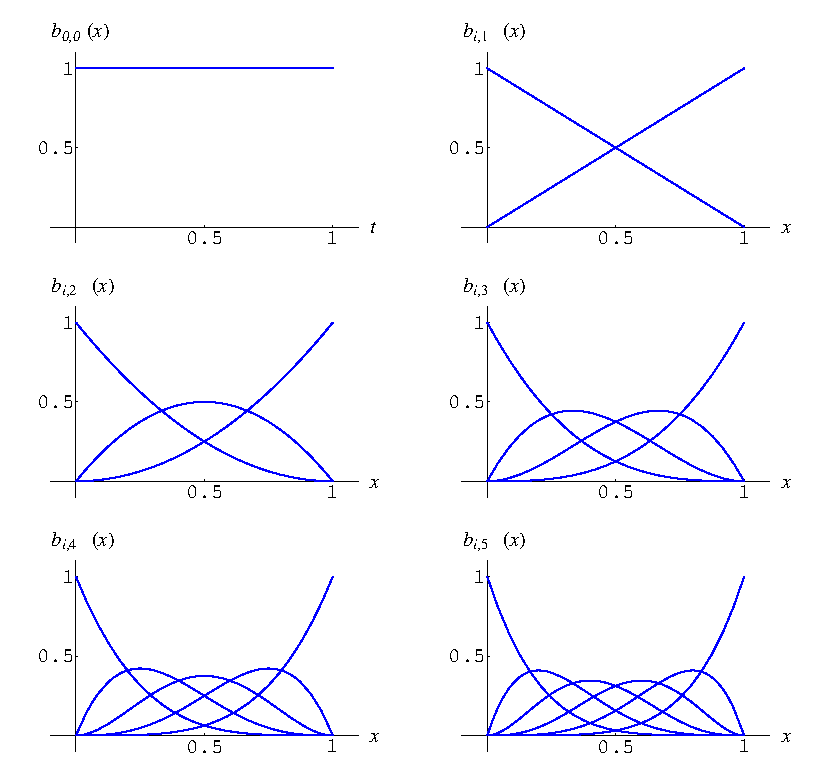
\includegraphics[width=\textwidth]{fig/BernsteinPol}
\caption{The Bernstein polynomials up to order $n=5$.\label{fig:BerPol}}
\end{center}
\end{figure}
\subsection{B\'ezier splines}
B\'ezier splines are curves defined on an interval for a parameter $t\in [0,1]$.
They are controlled by points that contribute to the curve parametrized by $t$
with a fixed weighting function in $t$. Two point, e.g., produce a straight
line, a so called linear B'ezier curve, to read
\[     \mathbf{B}(t)=\mathbf{P}_0 + t(\mathbf{P}_1-\mathbf{P}_0)=(1-t)\mathbf{P}_0 + t\mathbf{P}_1 \mbox{ , } t \in [0,1] \]
A cubic B\'ezier spline reads
\[     \mathbf{B}(t)=(1-t)^3\mathbf{P}_0+3(1-t)^2t\mathbf{P}_1+3(1-t)t^2\mathbf{P}_2+t^3\mathbf{P}_3 \mbox{ , } t \in [0,1]\]
A B\'ezier curve of degree $n$ reads
\[ \mathbf{B}(t)=\sum_{i=0}^n \binom{n}{i}(1-t)^{n-i}t^i\mathbf{P}_i =(1-t)^n\mathbf{P}_0+\binom{n}{1}(1-t)^{n-1}t\mathbf{P}_1+\cdots+t^n\mathbf{P}_n \mbox{ , } t \in [0,1]\]
Observe that in order to adjust the path the curve must follow you have to move
the control points. The extension to surfaces is straight forward
\[ x(s,t)=\sum_{i=0}^n \sum_{j=0}^m B_i^n(s) \; B_j^m(t) \; \mathbf{k}_{i,j}\]
where the $B_i^n(\nu)$ are the Bernstein polynomials and the $\mathbf{k}_{i,j}$ are the $(n+1)(m+1)$ control points.
\subsection{Legendre Polynomials}
Legendre polynomials are defined as
\begin{equation}
	    P_n(x) = \frac{1}{2^n n!}\frac{d^n}{dx^n } \left[ (x^2 -1)^n \right]
	\label{eq:legendre}
\end{equation}
They derive from the solution of the following differential equation
\[\frac{d}{dx} \left[ (1-x^2)\frac{d}{dx} P_n(x) \right] + n(n+1)P_n(x) = 0\]
Legendre polynomials are orthogonal on the interval $[-1,1]$, i.e.
\[     \int_{-1}^{1} P_m(x) P_n(x)\,dx = \frac{2}{2n + 1} \delta_{mn} \]
holds.

The first six Legendre polynomials read
\begin{eqnarray*}
 	P_0(x)=1\\
	P_1(x)=x\\
	P_2(x)=\frac{1}{2} (3x^2-1) \\
	P_3(x)=\frac{1}{2} (5x^3-3x) \\
	P_4(x)=\frac{1}{8} (35x^4-30x^2+3)\\
	P_5(x)=\frac{1}{8} (63x^5-70x^3+15x)
\end{eqnarray*}
\section{Numerical integration}
Numerical integration must be used if:
\begin{itemize}
	\item The integral cannot be evaluated analytically
	\item The integrand is not given in analytical form but rather
		numerically with a certain number of dicrete values
\end{itemize}
		
\subsection{Trapezoid quadrature}
This method consists in replacing the given function $f(x)$ by a set of lines connecting the sample points and then to sum all the trapezoid areas to approximate the integral, to give
\begin{eqnarray*}
	\int_{x_{i-1}}^{x_i}f(x)dx&\approx &\frac{f_{i-1}+f_i}{2}\Delta x_i\\
	\Delta x_i&=&x_i-x_{i-1}
\end{eqnarray*}
$[a,b]$ be the interval of integration. With $x_0=a,\; x_1,\dots,\; x_n=b$ we have
\begin{equation}
	\int_{a}^{b}f(x)dx\approx \sum_{i=1}^n\frac{f_{i-1}+f_i}{2}\Delta x_i
	\label{eq:trapez}
\end{equation}
Suppose that we have regularly spaced sample points
\[ \Delta x_i=\Delta x=\frac{b-a}{n} \]
Then (\ref{eq:trapez}) reads
\[\int_a^bf(x)dx\approx\frac{\Delta x}{2}\left[ f_0+f_n+2\sum_{i=1}^{n-1}f_i\right]\]
This does not allow to tell about the integration error. For this we have to
expand the function into a Taylor series to first order and one replaces the
function by a secant neglecting second order terms in $\Delta x$. One can show
that
\begin{equation}
	\int_a^bf(x)dx=\frac{\Delta x}{2}\left[ f(a)+f(b)+2\sum_{i=1}^{n-1}f(x_i)\right]
	-\frac{(\Delta x)^2}{12}(b-a)f''(\bar{x})-{\cal O}(\Delta x^4)
	\label{eq:order4}
\end{equation}
where $\bar{x}\in[a,b]$. In most cases one obtains a better approximation
of the integral, if one writes for the second derivative
\[ f''(\bar{x})=\frac{f'(a)-f'(b)}{b-a} \]
to give
\begin{equation}
        \int_a^bf(x)dx=\frac{\Delta x}{2}\left[ f(a)+f(b)+2\sum_{i=1}^{n-1}f(x_i)\right]
        -\frac{(\Delta x)^2}{12}\left[ f'(b)-f'(a)\right]
        \label{eq:order4apr}
\end{equation}
(\ref{eq:order4apr}) is the trapezoid form with corrections at the
endpoints. With this the methods becomes a 4th order method
%\subsection{Example}
\subsection{Integration using Interpolation}
We consider an interpolating polynomial with the support points given as
$a\le x_0\le x1\le\dots\le x_n\le b$
and, e.g. Lagrange polynomials as interpolation functions
\[ p_n[x]=\sum_{k=0}^nf[x_k]L_k[x]\]
Integration of the polynomial yields
\[ Q-n=\int_a^bp_n[x]dx=\sum_{k=0}^nf[x_k]\int_a^bL_k[x]dx=(b-a)\sum_{k=0}^nw_kf[x_k] \]
where the weights are defined as
\[ w_k=\frac{1}{(b-a)}\int_a^bL_k[x]dx\]

\begin{note}{}
If $f(x)$ is a polynomial of degree $<n+1$, then $p_n(x)$ is exact, and thus
also $Q_n$ is exact.
\end{note}
\subsection{Simpson's rule}
This method consists in replacing the function $f(x)$ between $x_{i-1}$ and
$x_{i+1}$ by a parabola passing through $f_{i-1}$, $f_i$, and $f_{i+1}$. One
can show the Simpson rule by a Taylor expansion of the integral. To this end we
write
\[ I(x)=\int_a^x f(x')dx'\]
It is
\[ \frac{dI(x)}{dx}=f(x)\]
The integral over the interval between $x_{i-1}$ and $x_{i+1}$ can now be written as
\[ A_i =I(x_{i+1})-I(x_{i-1})\]
If we do this for all intervals and sum, we get
\[\int_a^bf(x)dx=\frac{\Delta x}{3} \left[
f(a)+f(b)+4 \sum_{\substack{i=1\\ odd}}^{n-1} 
A_i+2 \sum_{\substack{i=2 \\ even}}^{n-2}A_i\right]+{\cal O}(\Delta x^4)\]

\subsection{Gau{\ss} quadrature}
This very precise method uses non uniformly distributed discretization points,
which are chosen to the best convenience. This method can be applied when the
integrand $f(x)$ is known analytically or if its values are known exactly where
the support points for the method have to be located. It might not be applied,
whenever a discrete representation of $f(x)$ does not fulfil these
requirements.

As we have already shown in the previous section, one can use an interpolation
of the function $f(x)$ in terms of polynomials, in order to write the integral
of this function as a weighted sum over its function values at specific points
\[ \int_{a}^{b}f(x)dx=C\sum_{k=1}^nw_kf(x_k)\]
where $C$ is proportional to $b-a$. The weighting factors $w_k$ depend on the
specific function that approximates $f(x)$. These are straight line segments is
the case of trapezoid quadrature, or parabolas in case of the method by
Simpson.

In the method by Gauss $f(x)$ is approximated by a basis of orthogonal
polynomials. The $x_i$ are the roots of these polynomials and thus are
irregularly spaced. One can use any kind of polynomials, e.g. Jacobi,
Tchebychev, Laguerre, Hermite\dots, but the most often used are those of
Legendre. These are defined in the interval $[-1,1]$. To this end we have to
change the variable, which is $x\in[a,b]$, by means of a linear transformation
to become $\xi\in[-1,1]$. This transformation reads
\[x=\frac{b+a}{2}+\frac{b-a}{2}\xi \]

Thus we have
\[\int_a^bf(x)dx=\frac{b-a}{2}\sum_{k=1}^{n}w_kf(x_k)\]
where the $w_k$ and the $\xi_k$ are given in the following table
\begin{center}
\begin{tabular}{|c|c|c|}
\hline
n&$\pm\xi_k$&$w_k$\\\hline
2&0.5773502692&1.0000000000\\\hline
3&0.0000000000&0.8888888889\\
 &0.7745966692&0.5555555556\\\hline
4&0.8611363116&0.3478548451\\
 &0.3399810436&0.6521451549\\\hline
5&0.0000000000&0.5688888889\\
 &0.5384693101&0.4786286705\\
 &0.9061798459&0.1713244924\\\hline
\end{tabular}
\end{center}

We shall not derive this method but rather give some arguments why it works.
One can show that the method is exact for polynomials of order $2n-1$. To see
this take such a polynomial $p(x)$ and represent it the following way
\[ p(x)=q(x)P_n(x) +r(x)\]
where $P_n(x)$ is a Legendre polynomial of order $n$, $q(x)$ is a polynomial of
order $n-1$ as well as is the rest $r(x)$. 
We thus have
\[ \int_{-1}^1p(x)dx=\int_{-1}^1q(x) P_n(x) dx+\int_{-1}^1r(x)dx=\int_{-1}^1r(x)dx\]
Now choose as support points the roots of $P_n(x)$ and we have the same result
from the quadrature formula
\[ \sum_{k=1}^nw_kp(x_k)=\sum_{k=1}^nw_kq(x_k)P_n(x_k)
+\sum_{k=1}^nw_kr(x_k)=\sum_{k=1}^nw_kr(x_k)\]
Now, the interpolation quadrature
formula of $x_k$ has accuracy of $2n-1$, and delivers the exact value for the
polynomial $L_k(x)^2$. Therefore we have
\[ w_k=\int_{-1}^1L_k(x)^2dx=\int_{-1}^1\prod_{\substack{j=1\\ j\neq
k}}\left(\frac{x-x_j}{x_k-x_j}\right)^2=\sum_{\mu=1}^nw_\mu L_k(x_\mu)^2\]

This gives a recipe how the $x_k$ and the $w_k$ must be chosen to get the
desired accuracy.
\subsection{Integrals of functions with multiple variables}
The multidimensional integral
\[ \int_{a_n}^{b_n}\ldots\int_{a_2}^{b_2}
\int_{a_1}^{b_1}f(x_1,x_2,\ldots,x_n)dx_1dx_2\cdots dx_n\]
must be progressively replaced by a quadrature formula
\[ \sum_{i_1=0}^{k_1}w_{i_1}\int_{a_2}^{b_2}\ldots
\int_{a_n}^{b_n}f(x_{i_1},x_2,\ldots,x_n)dx_1dx_2\cdots dx_n\]
to give
\[ \sum_{i_1=0}^{k_1}\sum_{i_2=0}^{k_2}\ldots
\sum_{i_n=0}^{k_n} w_{i_1} w_{i_2}\ldots w_{i_n}
f(x_{i_1},x_ {i_2},\ldots,x_ {i_n})\]
For high dimensional spaces of the function argument this can very easily end
in a tremendous computational load. In this case other methods must be provided
which are not subject of the discussion here.

%\chapter{Vollständige normierte Orthogonalsysteme (VNOS)}
Es sei eine Funktionenfolge $\{\varphi_{\nu}(x)$ mit dem diskreten Laufindex
$\nu$ und einem gemeinsamen Definitionsbereich $a\le x\le b$ gegeben. Alle
Elemente aus $\{\varphi_{\nu}(x)\}$ unterliegen denselben Einschränkungen.
Diese können z.B. in Form von Symmetrieeigenschaften oder Randbedingungen
vorliegen.

\end{appendices}
\end{document}